%====================================================
%
% Author: DR. XAVIER NOUMBISSI NOUNDOU
%
%====================================================
\documentclass[10pt, a4paper]{bookest}
\NeedsTeXFormat{LaTeX2e}
\makeindex

%---------------------------- PACKAGE INCLUSION -------------------------------
% This group renders characters clearer and more precise

\RequirePackage[bitstream-charter,cal,expert]{mathdesign}
\RequirePackage{makeidx}
\RequirePackage{latexsym}

\usepackage{geometry} % to change the page dimensions
\geometry{a4paper,
		  %showframe=true,
		  %margin=3cm,
		  %a4paper,
		  %total={170mm,257mm},
		  top=4.15em,
		  left=5.5em,
		  right=5.5em,
		  bottom=3.39em
		  }

\usepackage[default]{cantarell}
\usepackage{graphicx}
\usepackage[french]{babel}
\usepackage{xspace}
\usepackage[parfill]{parskip} % Activate to begin paragraphs with an empty line rather than an indent
\usepackage{paralist} % very flexible & customisable lists (eg. enumerate/itemize, etc.)
\usepackage{listings} % for lstset definitions
\usepackage{url}
\usepackage{subfig} % make it possible to include more than one captioned figure/table in a single float
\usepackage{epsfig}
\usepackage{booktabs}
%\usepackage{enumitem} %funny itemize icons
\usepackage{verbatim}

\usepackage{amsmath}
\newcommand{\mathbold}[1]{\text{\textbf{#1}}}

\usepackage{xcolor}
\definecolor{yerothColorOrange}{RGB}{242, 161, 0}   
\definecolor{yerothColorBlue}{RGB}{77 , 93 , 254}
\definecolor{yerothColorRed}{RGB}{254, 48 , 48}
\definecolor{yerothColorGray}{RGB}{198, 198, 198}
\definecolor{yerothColorDarkgray}{RGB}{60, 60 , 60}
\definecolor{yerothColorIndigo}{RGB}{83, 0, 125}
\definecolor{yerothColorGreen}{RGB}{2  , 160, 70}
\definecolor{forestgreen}{RGB}{2,160,70}    
\definecolor{mediumblue}{RGB}{7,43,205}    
\definecolor{firebrickred}{RGB}{178,34,34}
\definecolor{listingray}{gray}{0.9}
\definecolor{lbcolor}{rgb}{0.9,0.9,0.9}
\definecolor{darkgreen}{rgb}{0,0.35,0}
\definecolor{medgreen}{rgb}{0,0.5,0}
\definecolor{lightgreen}{rgb}{0.5,0.7,0.5}
\definecolor{pmcolour}{rgb}{0.5,0.7,0.5}
\definecolor{medgrey}{rgb}{0.6,0.6,0.6}
\definecolor{purplish}{rgb}{0.4,0,0.6}
\definecolor{brightred}{rgb}{1,0.2,0.2}

\usepackage{pagecolor}

\newcommand{\diplominformatiker}{Diplom--Informatiker\xspace}

\newcommand{\diplinfn}{DR.\xspace}

\newcommand{\pos}{syst\`eme--logiciel ERP\xspace}

\newcommand{\yerothlabs}{\textsc{Yeroth--R\&D}\xspace}

\newcommand{\yerotherptitle}{Yeroth--erp--$3.0$\xspace}

\newcommand{\yerotherpalerttroiszero}{\textcolor{yerothColorBlue}{\sc YEROTH--ERP--ALERT--$3.0$}\xspace}

\newcommand{\yerothpos}{\textcolor{yerothColorBlue}{\sc YEROTH--ERP--$3.0$}\xspace}

\newcommand{\myfullacademicname}{DR. XAVIER NOUMBISSI NOUNDOU\xspace}

\usepackage{hyperref}
\hypersetup{
    colorlinks,
	pagebackref,
    citecolor=medgreen,
    linkcolor=purplish,
    breaklinks,
    pdftex,
    bookmarks,
    plainpages=false,
	pdftitle={Guide de l'Utilisateur ''Manager'' de \yerothpos par \myfullacademicname},
    pdfauthor={DR. XAVIER NOUMBISSI NOUNDOU}
}

%--------------------------------------------------------------------------------

%---------------------------- COMMANDS DEFINITION -------------------------------

\newcommand{\junit}{\texttt{\textbf{JUnit}}\xspace}
\newcommand{\company}[1]{\textbf{#1}\xspace}
\newcommand{\diplinf}{\textsc{Dipl.-Inf.}\xspace}

\newcommand{\emphbf}[1]{\textbf{#1}\xspace}
\newcommand{\emphit}[1]{\emph{\textit{#1}}\xspace}
\newcommand{\mycheckmark}[1]{\textcolor{#1}{$\checkmark$}\xspace}
\newcommand{\mytimes}[1]{\textcolor{#1}{$\times$}\xspace}
\newcommand{\mytimespartial}[1]{\textcolor{#1}{partiel}\xspace}
\newcommand{\boldsc}[1]{\textbf{\textsc{#1}}\xspace}

\newcommand{\myenumitem}[1]{\emph{#1}\xspace}

\newcommand{\bergmann}{Bergmann Automaten GmbH\xspace}
\newcommand{\siemens}{\textsc{Siemens} Medical Solutions\xspace}
\newcommand{\watformlab}{Watform Lab\xspace}
\newcommand{\uwaterloo}{University of Waterloo\xspace}

\newcommand{\yeroth}{\textcolor{yerothColorBlue}{\sc YEROTH--ERP--$3.0$}\xspace}
\newcommand{\yerothalert}{\emph{yeroth--erp--alert--3.0}\xspace}
\newcommand{\mysql}{MySQL\xspace}
\newcommand{\depot}{d\'ep\^ot\xspace}
\newcommand{\depots}{d\'ep\^ots\xspace}
\newcommand{\bouton}[1]{"\textbf{#1}"\xspace}
\newcommand{\field}[1]{"\emph{\textbf{#1}}"\xspace}

\newcommand{\role}{r\^ole\xspace}
\newcommand{\roles}{r\^oles\xspace}
\newcommand{\manager}{\emph{Manager}\xspace}
\newcommand{\gestionairedestocks}{\emph{GestionaireDeStocks}\xspace}
\newcommand{\magasinier}{\emph{Magasinier}\xspace}
\newcommand{\caissier}{\emph{Caissier}\xspace}
\newcommand{\vendeur}{\emph{Vendeur}\xspace}
\newcommand{\admin}{\emph{Administrateur}\xspace}

\newcommand{\qt}{Qt$5.11$\xspace}

\newcommand{\managerb}{\emph{\textbf{Manager}}\xspace}
\newcommand{\gestionairedestocksb}{\emph{\textbf{GestionaireDeStocks}}\xspace}
\newcommand{\vendeurb}{\emph{\textbf{Vendeur}}\xspace}
\newcommand{\caissierb}{\emph{\textbf{Caissier}}\xspace}
\newcommand{\administrateurb}{\emph{\textbf{Administrateur}}\xspace}
\newcommand{\magasinierb}{\emph{\textbf{Magasinier}}\xspace}

\newcommand{\utilisateurs}
	{\textcolor{blue}{\textbf{\emph{R\^oles ayant acc\`es \`a la fonctionalit\'e}}}\xspace}

\newcommand{\facon}{fa\c{c}on\xspace}

\newcommand{\obligatoire}{\textcolor{firebrickred}{\textbf{\emph{[obligatoire]}}}\xspace}

\newcommand{\lienadmin}{\admin~\ref{sec:utilisateurs-ladministrateur}\xspace}
\newcommand{\liencaissier}{\caissier~\ref{sec:utilisateurs-lecaissier}\xspace}
\newcommand{\liengestionnairedesstocks}{\gestionairedestocks~\ref{sec:utilisateurs-gestionairedestocks}\xspace}
\newcommand{\lienmagasinier}{\magasinier~\ref{sec:utilisateurs-lemagasinier}\xspace}
\newcommand{\lienmanager}{\manager~\ref{sec:utilisateurs-lepatron}\xspace}
\newcommand{\lienvendeur}{\vendeur~\ref{sec:utilisateurs-vendeur}\xspace}

\newcommand{\deja}{d\'ej\`a\xspace}

\newcommand{\yerothfield}[1]{\textbf{\emph{#1}}\xspace}

\newcommand{\procparagraph}[1]
	{\paragraph{ \mycheckmark{forestgreen} \emph{\textcolor{forestgreen}{#1}}}}

\newcommand{\xavier}{Xavier NOUMBISSI NOUNDOU\xspace}

\newcommand{\reference}{r\'ef\'erence\xspace}

\newcommand{\cmup}{\textbf{CMUP}\xspace}
\newcommand{\dpfdpo}{\textbf{DEF\_DEO}\xspace}
\newcommand{\fifo}{\textbf{FIFO}\xspace}
\newcommand{\lifo}{\textbf{LIFO}\xspace}

\newcommand{\fenetre}{fen\^etre\xspace}
\newcommand{\uielemone}[1]{\textcolor{medgreen}{\emph{#1}}\xspace}
\newcommand{\uielemtwo}[1]{\textcolor{mediumblue}{\texttt{#1}}\xspace}

\newcommand{\nxsection}[1]{\section{#1}\xspace}
\newcommand{\nxsubsection}[1]{\subsection{#1}\xspace}

\newcommand{\chapintro}[1]{
\begin{center}
\parbox{35em}{
\textcolor{yerothColorIndigo}{#1}
}\xspace
\end{center}}

%\usepackage{makeidx} % Used to generate the index
%\makeindex % Generate the index which is printed at the end of the document

%--------------------------------------------------------------------------------

% Set font to avant-garde
%\renewcommand*\rmdefault{pag}

\usepackage[T1]{fontenc}

%Remove widows and orphants
\clubpenalty = 10000
\widowpenalty = 10000
\displaywidowpenalty = 10000

\begin{document}
\frontmatter\pagestyle{plain}
\title{\textcolor{medgreen}{\textsc{Syst\`eme--Logiciel ERP
		\\ \vspace*{1.5cm}(\yeroth)\\}
		\vspace*{3cm}
	Guide de l'Utilisateur\\ \vspace{1em} << Manager >> \\
	\vspace*{0.1cm}}
	{\small Version du --~$07$ Juin $2018$~--}}

\begin{titlepage}
\maketitle
\vspace{\stretch{2}}
\centering
\copyright\ \textsc{\myfullacademicname}
\end{titlepage}

% TABLE OF CONTENTS
\cleardoublepage
\phantomsection
\addcontentsline{toc}{chapter}{\contentsname}
\begingroup
\color{medgreen}
\tableofcontents
\endgroup

% LIST OF FIGURES
\cleardoublepage
\phantomsection
\addcontentsline{toc}{chapter}{\listfigurename}
\begingroup
\color{medgreen}
\listoffigures
\endgroup

% LIST OF TABLES
\cleardoublepage
\phantomsection
\addcontentsline{toc}{chapter}{\listtablename}
\begingroup
\color{medgreen}
\listoftables
\endgroup

\cleardoublepage
\phantomsection
\addcontentsline{toc}{chapter}{\`A propos de l'auteur}
\chapter*{\`A propos de l'auteur}\label{chap:biography}
\index{\`a propos de l'auteur}
\index{biographie de l'auteur}

\begin{figure}[!htpb]
\centering
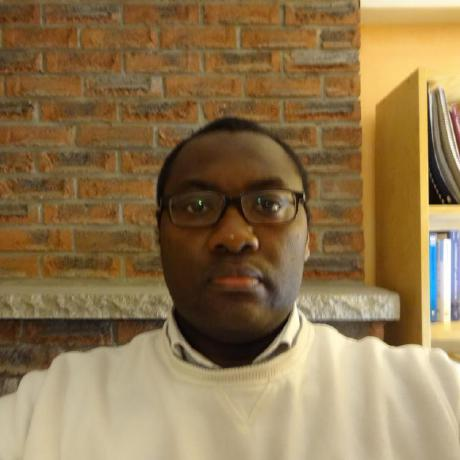
\includegraphics[scale=0.63]{images/XavierNOUNDOU-2}
\caption{Portrait de Xavier}~\label{fig:xaviernoumbis}
\end{figure}


\mainmatter

\chapter{Introduction}\label{chap:introduction}

\yeren est un syst\`eme logiciel de gestion des
stocks et de gestion des ventes. Il permet
d'ex\'ecuter des mouvements de stocks, et de
vendre des articles en stocks.

Une entreprise doit poss\'eder au minimum d'un stock
d'articles, d'un d\'ep\^ot ou d'une boutique pour utiliser
\yeren de fa\c{c}on efficace.\\

\begin{figure}[!htpb]
	\centering
	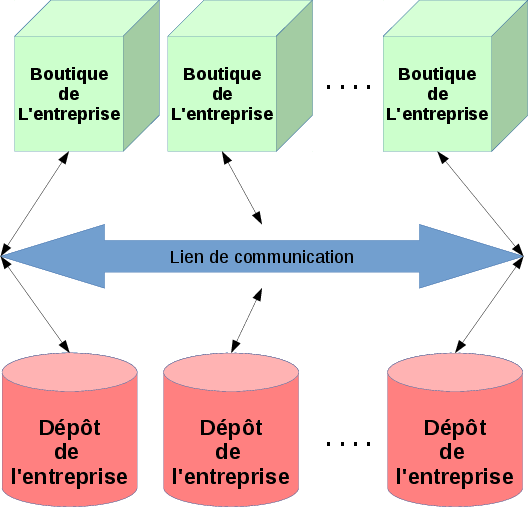
\includegraphics[scale=0.63]{images/architecture-enterprise-yeren.png}
	\caption{Un mod\`ele d'architecture d'une entreprise}\label{fig:architecture-enterprise-yeren}
\end{figure}

La figure~\ref{fig:architecture-enterprise-yeren} illustre
un mod\`ele g\'en\'erique d'entreprise o\`u les d\'ep\^ots
et les boutiques de l'entreprise sont en communication.

Les activit\'es principales de l'entreprise sont les suivantes:
\begin{enumerate}[1)]
	\item \emphbf{les sorties de stocks:} sortie d'articles
		d'une unit\'e (boutique ou d\'ep\^ot) pour r\'eception par un client
	\item \emphbf{les transferts de stocks:} mouvement d'articles
		d'une unit\'e vers une autre unit\'e
	\item \emphbf{les ventes d'articles:} un client ach\`ete
		des articles qui lui sont ensuite remis.\\
\end{enumerate}

\yeren permet d'accomplir les t\^aches de gestion
des stocks et de gestion des ventes suivantes:
\begin{enumerate}[1)]
	\item \myenumitem{cr\'eer des alertes sur des p\'eriodes de temps}	
	\item \myenumitem{cr\'eer des alertes sur des quantit\'e en stocks}	
	\item \myenumitem{entrer un stock}
	\item \myenumitem{lister les stocks}
	\item \myenumitem{modifier un stock}
	\item \myenumitem{supprimer un stock}	
	\item \myenumitem{rechercher des articles ou des stocks}
	\item \myenumitem{transf\'erer des articles ou des stocks}	
	\item \myenumitem{vendre des articles}	
	\item \myenumitem{visualiser les \'etats de transactions d'articles
		(sorties ou transferts de stocks)}
	\item \myenumitem{acc\'eder aux tableaux de bords}
	\item \myenumitem{visualiser les \'etats de ventes d'articles}.\\
\end{enumerate}

\newpage

\section{Acc\`es au manuel de l'utilisateur}

La figure~\ref{fig:fenetre-principale-utilisateur-non-enregistre}
illustre la fen\^etre d'accueil de \yeren sans aucun utilisateur
enregistr\'e.\\

\begin{figure}[!htbp]
\centering
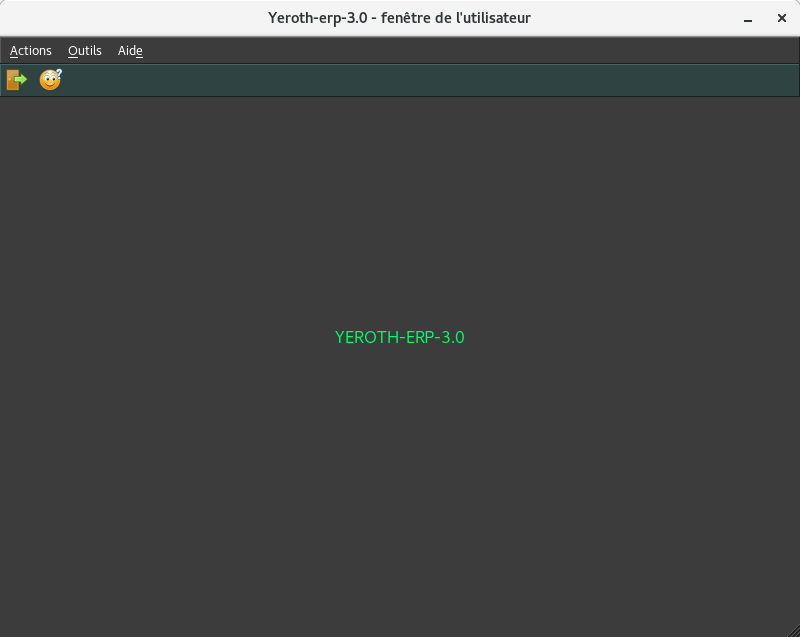
\includegraphics[scale=0.63]{images/yeren-fenetre-principale.png}
\caption{La fen\^etre d'acceuil sans aucun utilisateur enregistr\'e.}
\label{fig:fenetre-principale-utilisateur-non-enregistre}
\end{figure}

Il est requis qu'un utilisateur soit enregistr\'e
dans \yeren afin d'avoir acc\`es au manuel de l'utilisateur.

L'utilisateur de \yeren doit accomplir les op\'erations
suivantes afin d'avoir acc\`es au manuel de l'utilisateur:
\begin{enumerate}[1)]
	\item \`a partir de la fen\^etre d'accueil
		(voir figure~\ref{fig:fenetre-principale-utilisateur-non-enregistre}),
		cliquez sur le menu d\'eroulant '\textbf{Aide}'
	\item ensuite cliquez sur le lien '\textbf{Manuel de l'utilisateur (PDF)}'.
\end{enumerate}

\section{Structure de ce manuel de l'utilisateur}
Ce manuel de  l'utilisateur de \yeren est structur\'e
comme suit:

\begin{itemize}[\mycheckmark{purplish}]
	\item le chapitre~\ref{chap:utilisateurs} d\'ecrit
	les utilisateurs de \yeren et leurs \roles. 
	     
	\item le chapitre~\ref{chap:gestion-stocks} explicite
	les fonctionalit\'es de gestion des stocks

	\item le chapitre~\ref{chap:gestion-des-achats} parle
	de la gestion des achats
	
	\item le chapitre~\ref{chap:systeme-dalertes}
	pr\'esente le syst\`eme d'alertes sur les stocks
	
	\item le chapitre~\ref{chap:vendre} d\'ecrit comment
	conclure des ventes d'articles
	
	\item le chapitre~\ref{chap:sortir-articles} d\'ecrit
	comment proc\'eder \`a des sorties et transferts de stocks
	
	\item le chapitre~\ref{chap:vente} explicite comment
	rechercher et imprimer les \'etats de ventes d'articles
	
	\item le chapitre~\ref{chap:etats-des-sorties} explicite
	comment rechercher et imprimer les \'etats de sorties ou
	transferts d'articles
	
	\item le chapitre~\ref{chap:tableaux-de-bord} discute
	de la recherche et de la g\'en\'eration des rapports
	commerciaux de l'entreprise
	
	\item le chapitre~\ref{chap:informations-generales}
	explique comment avoir acc\`es aux d\'etails de
	l'utilisateur enregistr\'e, aux informations commerciales
	de l'entreprise, et enfin \`a la version de \yeren que
	l'on utilise
	
	\item le chapitre~\ref{chap:administration-logiciel}
	traite de l'administration du logiciel

	\item le chapitre~\ref{chap:problemes-connues}
	discute des probl\`emes connues de \yeren
	
	\item enfin, le chapitre~\ref{chap:conclusion} conclut
	ce manuel d'utilisation.
\end{itemize}


\chapter{Les R\^oles et Les Utilisateurs}\label{chap:utilisateurs}
\index{types de \roles}

\utilisateurs: \lienadmin, \liencaissier, \lienmagasinier, \lienpatron.\\

\chapintro{Ce chapitre d\'ecrit les diff\'erents types d'utilisateurs de
\yeren: \admin, \magasinier, \caissier, et \patron.}

\nxsection{Introduction}\label{sec:utilisateurs-introduction}

\yeren maintient les donn\'ees suivantes pour chaque utilisateur:
\begin{enumerate}[1)]
	\item l'\'email \optionel
	\item la bo\^ite postale
	\item le date de naissance \optionel
	\item le lieu de naissance \optionel
	\item la localisation (le site de l'entreprise o\`u l'employ\'e
	      est en fonction). Cette valeur ne peut \^etre \'edit\'ee.
	      Sa valeur est automatiquement remplie \`a partir de la
	      license d'installation.
	\item le nom
	\item le num\'ero de t\'el\'ephone 1 \optionel
	\item le num\'ero de t\'el\'ephone 2 \optionel
	\item le pays \optionel
	\item le pr\'enom	
	\item la province / \'etat
	\item le r\^ole dans \yeren (\admin, \magasinier, \caissier, ou \patron)
	\item le titre (Dr., Me., Mlle, Mme, Mr, Pr., Prof.)
	\item la ville \optionel
\end{enumerate}

\newpage

\nxsection{Le r\^ole ''Administrateur''}\label{sec:utilisateurs-ladministrateur}
\index{administrateur}
\index{LAdministrateur}

La figure~\ref{fig:fenetre-principale-admin} illustre la
fen\^etre d'acceuil d'un utilisateur avec le \role \admin,
apr\`es qu'il se soit enregistr\'e dans \yeren.\\

\begin{figure}[!htbp]
\centering
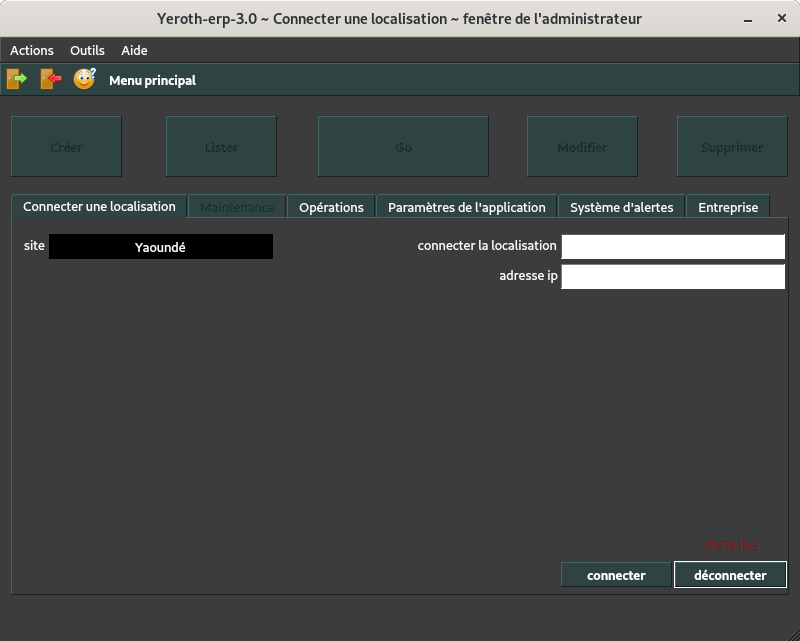
\includegraphics[scale=0.63]{images/yeroth-fenetre-administrateur.png}
\caption{La fen\^etre d'acceuil d'un administrateur.}
\label{fig:fenetre-principale-admin}
\end{figure}

Un utilisateur avec le \role "\admin" assume les
t\^aches de cr\'eer et de maintenir les objets suivants:
\begin{enumerate}[1)]
	\item les alertes (sur une p\'eriode de temps, ou sur une quantit\'e en stock)
	%\item les bons de commande
	\item les cat\'egories d'articles
	\item les clients
	\item les comptes utilisateurs
	\item les fournisseurs				
	\item les localisations (une localisation est un site de
	      l'entreprise o\`u se trouve un ou plusieurs stocks).\\   
\end{enumerate}

\newpage

\nxsection{Le r\^ole ''Manager''}\label{sec:utilisateurs-lepatron}
\index{patron}
\index{LePatron}

La figure~\ref{fig:yeren-fenetre-patron} illustre la fen\^etre
d'acceuil d'un utilisateur avec le \role \patron, 
apr\`es qu'il se soit enregistr\'e dans \yeren.\\

\begin{figure}[!htbp]
\centering
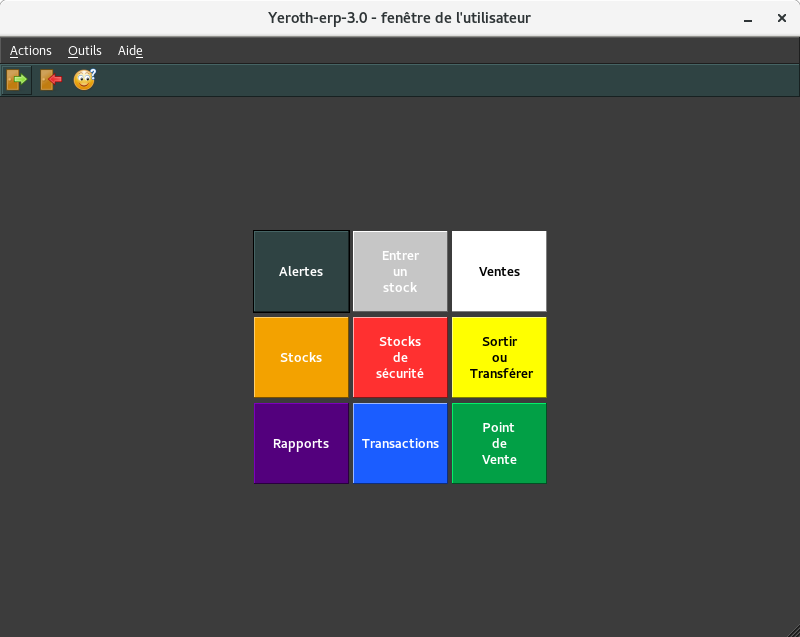
\includegraphics[scale=0.63]{images/yeren-fenetre-patron.png}
\caption{La fen\^etre d'acceuil d'un ''manager''}
\label{fig:yeren-fenetre-patron}
\end{figure}

Un utilisateur de \yeren avec le \role "\patron" a
acc\`es \`a toutes les fonctionalit\'es de \yeren. Il
cumule les t\^aches de d'administrateur, de magasinier,
et de caissier.

Le \role \patron est le seul \`a donner acc\`es aux
informations des ventes dans leurs totalit\'es, ainsi
qu'\`a la g\'en\'eration et \`a la consultation des
rapports commerciaux.

Le \role \patron est le seul \`a pouvoir consulter toutes
les alertes re\c{c}ues par les autres utilisateurs, et
\`a pouvoir les supprimer.

\newpage

\nxsection{Le r\^ole ''GestionaireDeStocks''}\label{sec:utilisateurs-gestionairedestocks}
\index{gestionaire de stocks}
\index{GestionaireDeStocks}

La figure~\ref{fig:yeren-fenetre-gestionairedestocks} illustre
la fen\^etre d'acceuil d'un utilisateur avec le \role \gestionairedestocks, 
apr\`es qu'il se soit enregistr\'e dans \yeren.\\

\begin{figure}[!htbp]
\centering
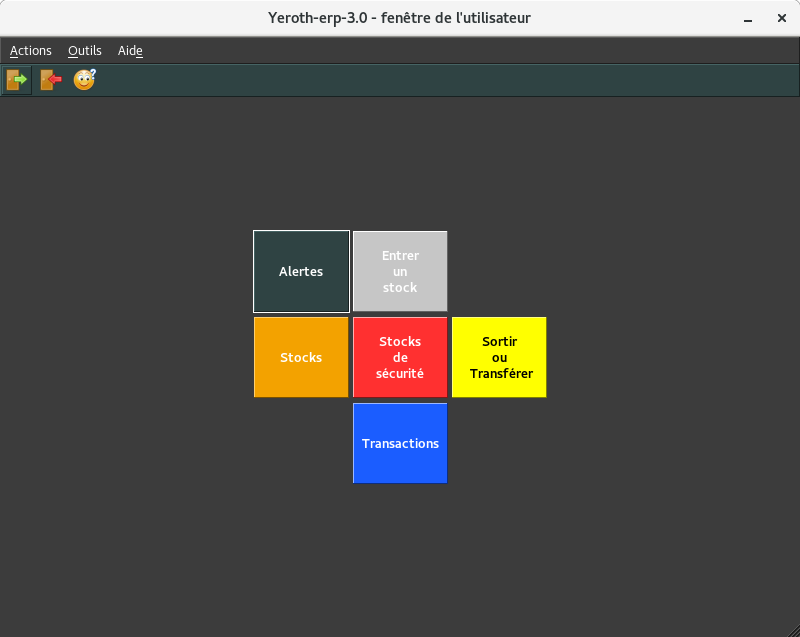
\includegraphics[scale=0.63]{images/yeren-fenetre-gestionairedestocks.png}
\caption{La fen\^etre d'acceuil d'un gestionaire de stocks}
\label{fig:yeren-fenetre-gestionairedestocks}
\end{figure}

\newpage

\nxsection{Le r\^ole ''Magasinier''}\label{sec:utilisateurs-lemagasinier}
\index{magasinier}
\index{LeMagasinier}

La figure~\ref{fig:yeren-fenetre-magasinier} illustre
la fen\^etre d'acceuil d'un utilisateur avec le
\role \magasinier, apr\`es qu'il se soit enregistr\'e
dans \yeren.\\

\begin{figure}[!htbp]
\centering
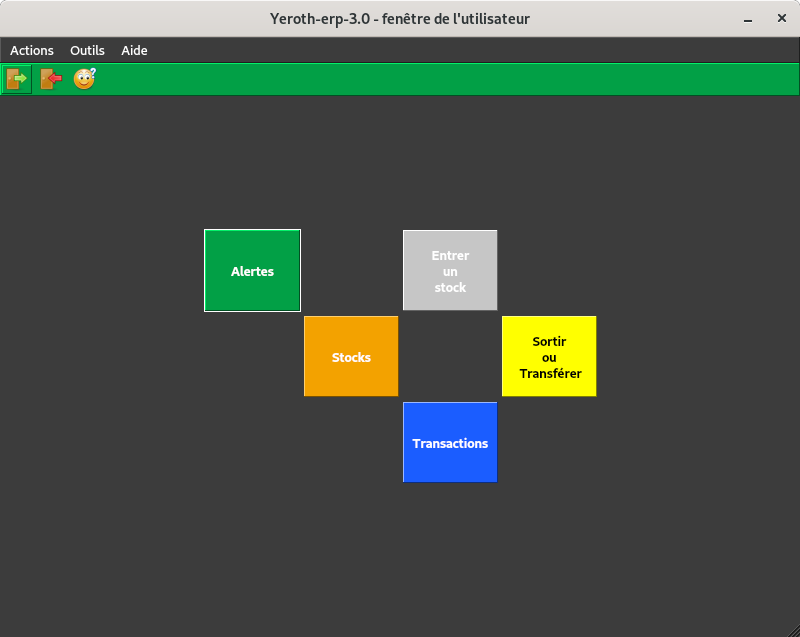
\includegraphics[scale=0.63]{images/yeren-fenetre-magasinier.png}
\caption{La fen\^etre d'acceuil d'un magasinier.}
\label{fig:yeren-fenetre-magasinier}
\end{figure}

Un utilisateur de \yeren avec le \role "\magasinier" assume les
t\^aches suivantes:
\begin{enumerate}[1)]
	\item lister des stocks
	\item modifier un stock
	\item rechercher des articles / stocks
	\item rechercher des transactions 
		(sorties de stocks ou transferts de stocks)
	\item sortir des articles / stocks
	\item supprimer un stock
	\item transf\'erer un stock
	\item visualiser des transactions
	(sorties de stocks ou transferts de stocks).\\
\end{enumerate}

\magasinier n'a pas acc\`es aux fonctions
\bouton{Administration}, \bouton{Ventes},
\bouton{Rapports}, et \bouton{Vendre}.

On remarque sur la Figure~\ref{fig:yeren-fenetre-magasinier}
que les boutons \bouton{Administration}, \bouton{Ventes},
\bouton{Rapports}, et \bouton{Vendre} sont d\'esactiv\'es.
	
\newpage

\nxsection{Le r\^ole ''Caissier''}\label{sec:utilisateurs-lecaissier}
\index{caissier}
\index{LeCaissier}

La figure~\ref{fig:fenetre-principale-caissier} illustre la
fen\^etre d'acceuil d'un utilisateur avec le \role \caissier,
apr\`es qu'il se soit enregistr\'e dans \yeren.\\

\begin{figure}[!htbp]
\centering
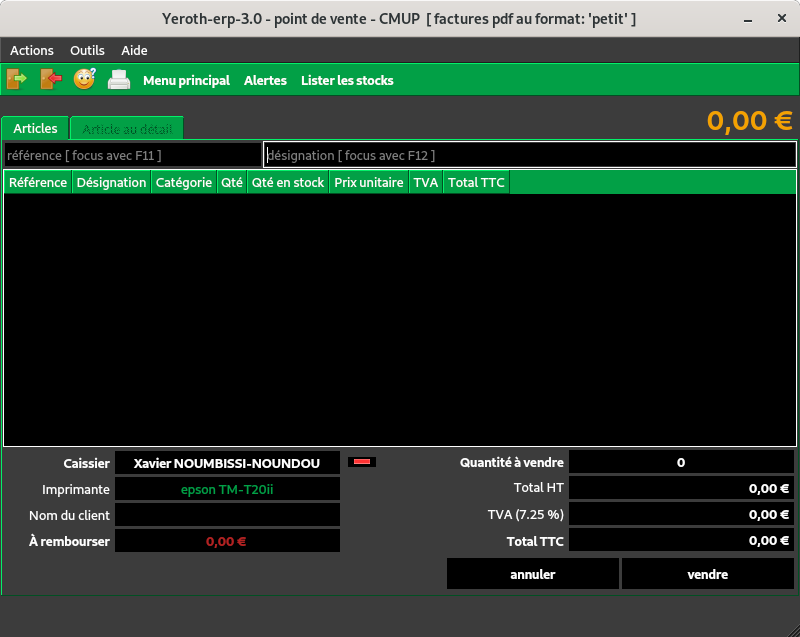
\includegraphics[scale=0.63]{images/yeren-fenetre-caissier.png}
\caption{La fen\^etre d'acceuil d'un caissier.}
\label{fig:fenetre-principale-caissier}
\end{figure}

Un utilisateur de \yeren avec le \role "\caissier" assume
les t\^aches suivantes:
\begin{enumerate}[1)]
	\item lister les stocks \`a partir de l'interface de vente	
	\item visualiser une facture proforma		
	\item imprimer une facture proforma
	\item vendre un ou plusieurs stocks (ou articles).\\
\end{enumerate}

\chapter{La Gestion des Stocks}\label{chap:gestion-stocks}
\index{la gestion des stocks}

\utilisateurs: \lienmagasinier.\\

\chapintro{Ce chapitre d\'ecrit comment avoir acc\`es aux
fonctionalit\'es de gestion des stocks et comment les utiliser.}

\nxsection{Introduction}

Les t\^aches de gestion des stocks sont illustr\'ees
dans le Tableau~\ref{tab:taches-fonctions}, en fonction
du r\^ole de l'utilisateur.\\

\begin{table}[!htbp]
\centering
\begin{tabular}{lccccc}
\textbf{T\^aches} 							& \managerb		 & \vendeurb	 		&	\gestionairedestocksb	& \magasinierb		& \caissierb 		\\ \hline
entrer un stock 							& \mycheckmark{blue} & 				 		& \mycheckmark{blue}			& 					&  				 	\\ \hline
supprimer un stock 							& \mycheckmark{blue} & 				 		& 							&					&  					\\ \hline
lister les marchandises 					& \mycheckmark{blue} &\mycheckmark{blue} 		& \mycheckmark{blue} & 	& \\ \hline
lister les stocks 							& \mycheckmark{blue} &\mycheckmark{blue} 		& \mycheckmark{blue}			& \mycheckmark{blue}	& \mycheckmark{blue} 	\\ \hline
modifier un stock 							& \mycheckmark{blue} & 				 		& \mycheckmark{blue}			& 					&  				 	\\ \hline
transf\'erer des stocks 					& \mycheckmark{blue} & 				 		& \mycheckmark{blue}			& \mycheckmark{blue}	&  				 	\\ \hline
sortir des stocks							& \mycheckmark{blue} & 				 		& \mycheckmark{blue}			& \mycheckmark{blue}	&  				 	\\ \hline
modifier la strat\'egie 					&  				 & 				 		& 							& 					&	 				\\ 
de gestion des stocks  						& \mycheckmark{blue} & \mytimespartial{blue}& \mytimespartial{blue}		& 					&  				 	\\ 
(ex.: \fifo, etc.)							&				 &				 		&							&					&					\\ \hline
vendre des marchandises 					& \mycheckmark{blue} & \mycheckmark{blue} 		&				 			& 					& \mycheckmark{blue} 	\\ \hline
acc\'eder aux  		 						& 				 &				 		&				 			& 					&  				 	\\ 
mouvements des stocks 	   		 			& \mycheckmark{blue} & 				 		&\mycheckmark{blue}				& \mycheckmark{blue}  	&				 	\\
\end{tabular}
\caption{Tableau des t\^aches et des r\^oles associ\'es
\`a la gestion des stocks}
\label{tab:taches-fonctions}
\index{t\^aches de gestion des stocks}
\end{table}

\nxsection{Les strat\'egies de gestion des stocks}\label{sec:strategies-gestion-stocks}
\index{strat\'egies de gestion des stocks}
\index{strat\'egie de sortie des articles}
\index{strat\'egie de vente des articles}
\index{strat\'egie de gestion des stocks ! \cmup}
\index{strat\'egie de gestion des stocks ! \dpfdpo}
\index{strat\'egie de gestion des stocks ! \fifo}
\index{strat\'egie de gestion des stocks ! \lifo}

\yeren impl\'emente $4$ strat\'egies pour g\'erer les stocks \`a
vendre ou \`a sortir:
\begin{enumerate}[1)]
	\item \cmup: Cours Moyen, Unit\'e Pond\'er\'ee.
	
		La strat\'egie \cmup affiche tous les 
		stocks de \facon (Cours
		Moyen, Unit\'e Pond\'er\'ee).\\
		
	\item \dpfdpo: Date of Expiration First, Date of Expiration Out.
	
		La strat\'egie \dpfdpo affiche les
		stocks \`a vendre ou \`a sortir selon
		le principe: les stocks avec des dates
		de p\'eremption les plus proches sont 
		les premiers \`a sortir.\\
		
	\item \fifo: First In, First Out. 
	
		La strat\'egie \fifo affiche les stocks
		\`a vendre ou \`a sortir selon le principe
		''\textbf{First In, First Out}'':
		Les stocks avec des dates d'entr\'ee en stock
		plus anciennes sont les premiers \`a sortir.\\
		
	\item \lifo: Last In, First Out.
	
		La strat\'egie \lifo affiche les stocks
		\`a vendre ou \`a sortir selon le principe
		''\textbf{Last In, First Out}'': 
		Les stocks avec des dates d'entr\'ee en stock
		plus r\'ecentes sont les premiers \`a sortir.\\
\end{enumerate}
\index{\cmup}
\index{\dpfdpo}
\index{\fifo}
\index{\lifo}

La strat\'egie de gestion des stocks se modifie
comme suit:

\begin{itemize}[\mycheckmark{purplish}]
	\item de \facon permanente dans
		la section 'administration' de \yerenpos.

	\item de \facon temporaire (\`a des fins de
		visualitation de l'ordre des sorties de
		stocks) dans la \fenetre 
		\textbf{'fiche des stocks'} de \yerenpos.
\end{itemize}

%\newpage

%-----------------------------------------------------------

\nxsection{Entrer un stock}
\index{entrer un stock}
\index{stock minimum}

\yeren entretient les donn\'ees suivantes pour chaque stock:
\begin{enumerate}[1)]
	\item la cat\'egorie \obligatoire
	\item la d\'esignation \obligatoire
	\item la date de p\'eremption du stock 
	\item le fournisseur 
	\item la localisation du stock
	\item le montant de la TVA d'un article 
	\item le prix de vente d'un article \obligatoire
	\item la quantit\'e intiale (nombre de lots, et quantit\'e par lot) \obligatoire
	\item la \reference
	\item la \reference du re\c{c}u d'achat
	\item le stock minimum: si cette quantit\'e
		est atteinte, alors le nombre de la colone 'Qt\'e totale'
		du stock est affich\'e en rouge.\\
\end{enumerate}

Il existe deux m\'ethodes pour entrer un stock dans \yeren:
\begin{enumerate}[1)]
	\item la $\mathbf{1^{\textbf{\`ere}}}$ \textbf{m\'ethode}
	est utilis\'ee pour entrer un stock d'articles \`a partir
	d'un formulaire vide
	
	\item la $\mathbf{2^{\textbf{\`eme}}}$ \textbf{m\'ethode}
	permet \`a l'utilisateur de r\'eutiliser la
	\yerenfield{cat\'egorie}, la \yerenfield{d\'esignation},
	le \yerenfield{prix d'achat}, le \yerenfield{prix de vente},
	la \yerenfield{TVA} si existante, et la \yerenfield{\reference}
	d'un stock de m\^eme nature d\'ej\`a existant.\\
\end{enumerate}

Les deux m\'ethodes sont les suivantes:

\begin{itemize}[\mycheckmark{purplish}]
	\item \textcolor{purplish}{$\mathbf{1^{\text{\`ere}}}$ \textbf{m\'ethode}}\\
		   \`A partir de la fen\^etre d'acceuil titr\'e
		   '\textbf{\yerotherptitle\ -- fen\^etre de l'utilisateur}'
		   (voir figure~\ref{fig:yeren-fenetre-patron}), cliquez
		   sur le boutton \bouton{Entrer un stock} pour obtenir un
		   formulaire vide afin d'entrer en stock. Le formulaire
		   obtenu est illustr\'e dans la figure~\ref{fig:formulaire-entrer-1}.\\
		   
		   Si vous entrez la \reference d'un article qui existe
		   \deja dans le stock, les informations suivantes sont
		   automatiquement remplies:
		   \begin{enumerate}[1)]
		   		\item la \yerenfield{d\'esignation}
		   		\item la \yerenfield{cat\'egorie} \\		   		
		   \end{enumerate}		    
		   
	      \begin{figure}[!htbp]
		  \centering
		  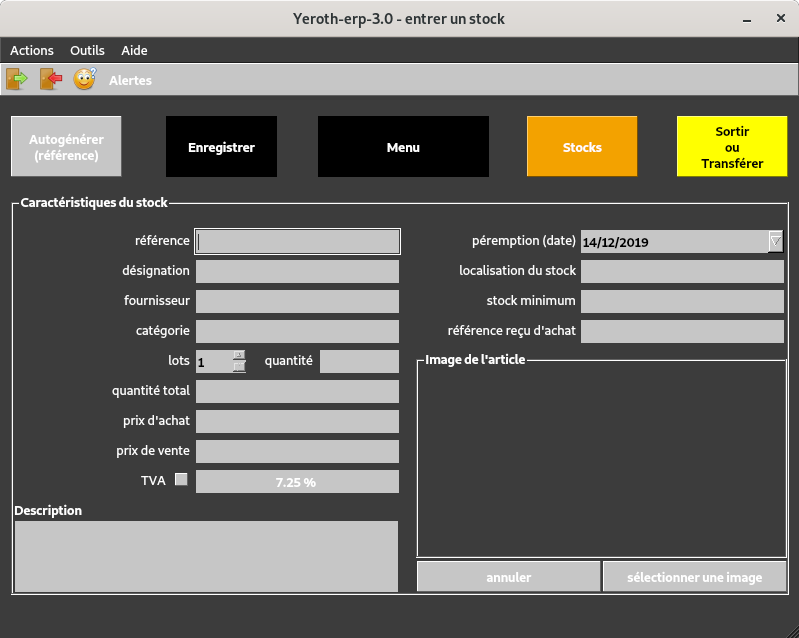
\includegraphics[scale=0.63]{images/yeren-fenetre-entrer.png}
		  \caption{Le formulaire vide pour entrer un stock.}
		  \label{fig:formulaire-entrer-1}
		  \end{figure}	     
	      
	\newpage	      
	      
	\item \textcolor{purplish}{$\mathbf{2^{\text{\`eme}}}$ \textbf{m\'ethode}}
		\begin{enumerate}[1)]
			\item \`A partir de la fen\^etre d'acceuil
			(voir figure~\ref{fig:yeren-fenetre-patron}),
			cliquez sur le boutton \bouton{Stocks}
			\item ensuite, s\'electionnez un stock en cliquant dessus une fois
			\item enfin, cliquez sur le le boutton \bouton{Entrer un stock}.\\
		\end{enumerate}				
		
		L\`a vous obtenez un formulaire partiellement rempli
	    avec les donn\'ees r\'eutilisables du stock s\'electionn\'e.
	    Le formulaire que vous obtenez est celui de la
	    figure~\ref{fig:formulaire-entrer-2}.\\
	    
	    \begin{figure}[!htbp]
		\centering
		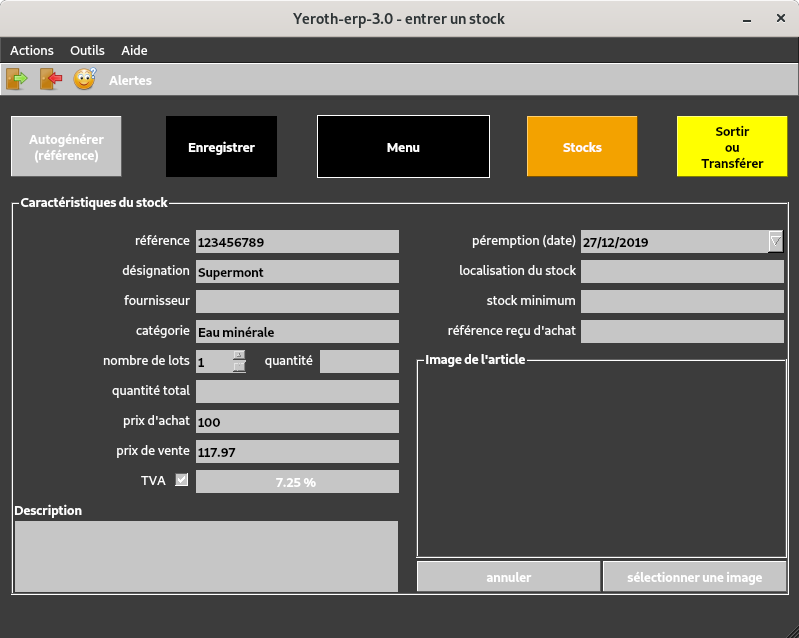
\includegraphics[scale=0.63]{images/yeren-fenetre-entrer-2.png}
		\caption{Le formulaire partiellement rempli pour entrer un nouveau stock.}
		\label{fig:formulaire-entrer-2}
		\end{figure}
\end{itemize}

\newpage

%-----------------------------------------------------------

\nxsection{Lister des stocks}
\index{fiche des stocks}
\index{lister des stocks}
\index{strat\'egie de gestions des stocks}
\index{visualiser la fiche des stocks}
\index{visualiser la liste des stocks}

La figure~\ref{fig:fenetre-lister} illustre la fen\^etre
d'acceuil de \yeren pour lister les stocks.

Le titre de cette fen\^etre explicite la strat\'egie
de gestion des stocks utilis\'ee pour vendre ou
sortir des articles: \cmup.\\

\begin{figure}[!htbp]
\centering
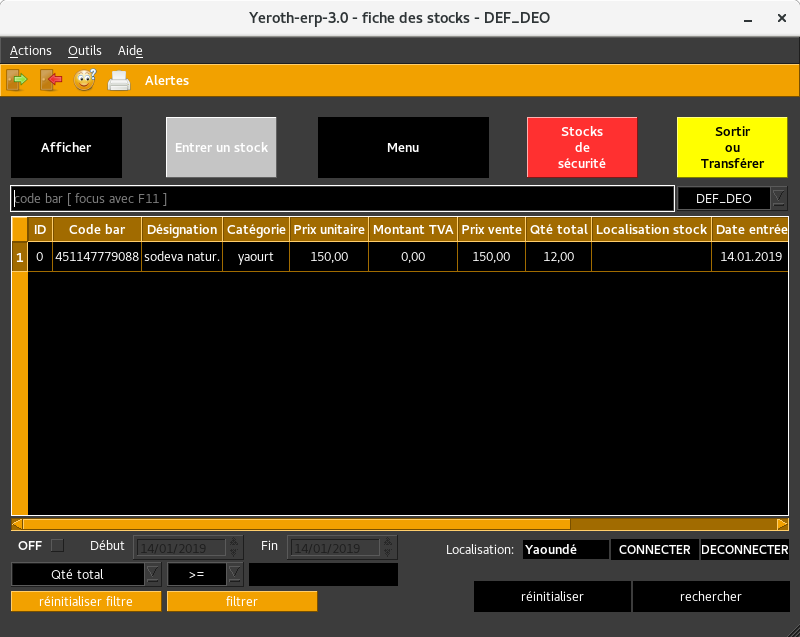
\includegraphics[scale=0.63]{images/yeren-fenetre-lister.png}
\caption{La fen\^etre pour lister les stocks.}
\label{fig:fenetre-lister}
\end{figure}

\`A partir d'une \fenetre quelconque qui y donne
acc\`es, l'acc\`es \`a la fonctionnalit\'e, 'Lister des stocks'
se fait avec au moins l'une des m\'ethodes suivantes: 

\begin{itemize}[\mycheckmark{purplish}]
	\item \textcolor{purplish}{$\mathbf{1^{\text{\`ere}}}$ \textbf{m\'ethode}}\\
		cliquez sur le lien \bouton{Lister des stocks}
		dans le menu d\'eroulant \textbf{Actions}\\

	\item \textcolor{purplish}{$\mathbf{2^{\text{\`eme}}}$ \textbf{m\'ethode}}\\
		cliquez sur le bouton \bouton{Stocks}.
\end{itemize}

\subsection{Les stocks list\'es en rouge}
Les stocks list\'es en \textcolor{firebrickred}{rouge} dans
la colone ''Qt\'e totale'' sont ceux dont la quantit\'e
minimale en stock a \'et\'e atteinte.

Les stocks list\'es en \textcolor{firebrickred}{rouge} dans
la colone ''Date p\'eremption'' sont ceux dont la date de
p\'eremption a \'et\'e atteinte.

\subsection{Les stocks list\'es en vert}
Les stocks list\'es en \textcolor{medgreen}{vert} dans la
colone ''Date p\'eremption'' sont ceux qui ont \'et\'e
s\'electionn\'es pour la vente par l'algorithme correspondant:
\dpfdpo.

Les stocks list\'es en \textcolor{medgreen}{vert} dans la
colone ''Date entr\'ee'' sont ceux qui ont \'et\'e
s\'electionn\'es pour la vente par lun des algorithmes
suivants: \fifo, \lifo.


%-----------------------------------------------------------
\newpage
\nxsection{Imprimer la fiche des stocks
	au format PDF}\label{sec:imprimer-liste-stocks}
\index{imprimer la fiche des stocks}
\index{imprimer la liste des stocks}

Il existe deux m\'ethodes pour imprimer la liste des
stocks qui appara\^it dans la fen\^etre titr\'ee
'\textbf{Yeren - Lister des stocks}'.

\begin{itemize}[\mycheckmark{purplish}]
	\item \textcolor{purplish}{$\mathbf{1^{\text{\`ere}}}$ \textbf{m\'ethode}}\\
		Cliquez sur le lien '\textbf{Imprimer la fiche des stocks}'
		qui se trouve dans le menu d\'eroulant '\textbf{Outils}'\\

	\item \textcolor{purplish}{$\mathbf{2^{\text{\`eme}}}$ \textbf{m\'ethode}}\\
		Cliquez sur l'ic\^one blanche repr\'esentant
		une 'imprimante'\\

	\item \textcolor{purplish}{$\mathbf{3^{\text{\`eme}}}$ \textbf{m\'ethode}}\\
		Pressez simultan\'ement les boutons \bouton{CTRL}
		et \bouton{P} de votre clavier.\\
\end{itemize}

Un fichier au format PDF ayant la liste des stocks affich\'ee
est alors g\'en\'er\'e.

%-----------------------------------------------------------
%\newpage
\nxsection{Rechercher un article ou un stock}
\index{rechercher un article}
\index{rechercher un stock}

Il existe deux m\'etodes pour rechercher un article / stock:
\begin{itemize}[\mycheckmark{purplish}]
	\item \textcolor{purplish}{$\mathbf{1^{\text{\`ere}}}$ \textbf{m\'ethode}}

	\begin{enumerate}[1)]
		\item cliquez sur le bouton \bouton{rechercher}
		\item ou bien cliquez sur le lien '\textbf{Rechercher un article}'
			dans le menu d\'eroulant \textbf{Outils}.\\
	\end{enumerate}
	
	L'utilisateur est alors conduit vers une petite fen\^etre de
	dialogue ou il peut introduire les mots cl\'es de sa recherche,
	ainsi que les param\`etres optionels suivants: la
	\yerenfield{cat\'egorie du stock}, la \yerenfield{d\'esignation du stock}
	et le \yerenfield{fournisseur du stock}.
	Ceci est illustr\'e dans la figure~\ref{fig:fenetre-rechercher-stock}.\\
	
	\begin{figure}[!htbp]
		\centering
		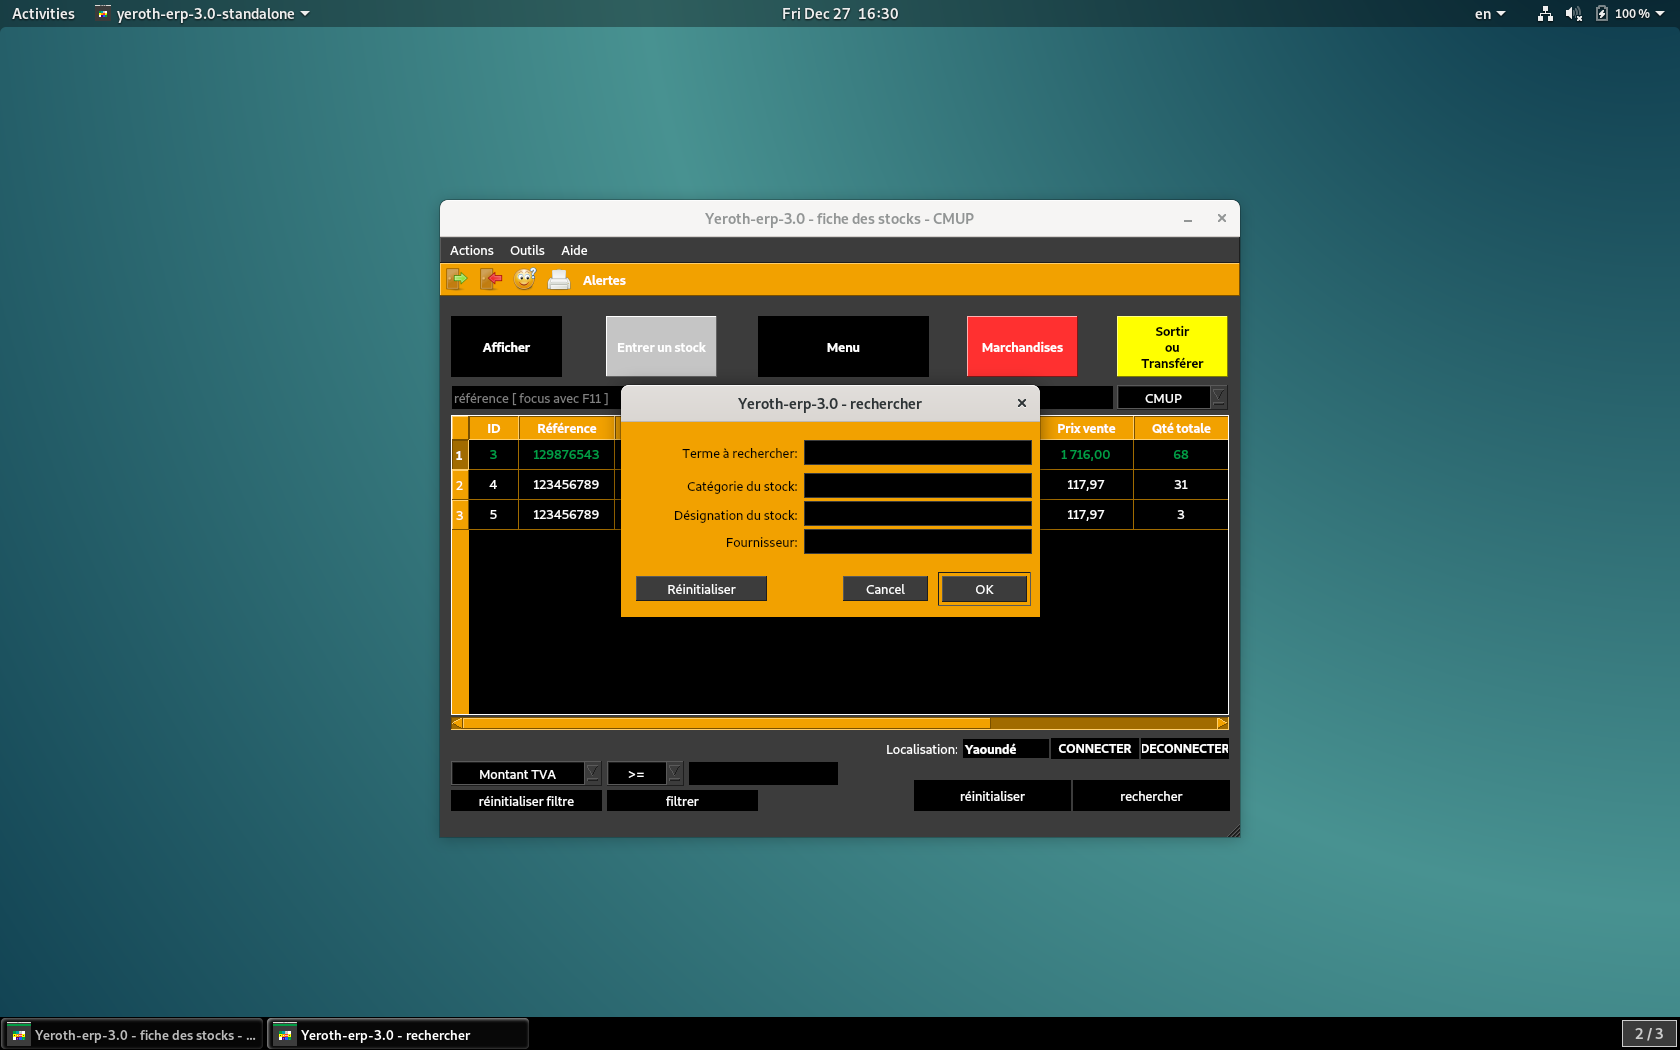
\includegraphics[scale=0.26]{images/yeren-rechercher-un-article.png}
		\caption{La fen\^etre pour rechercher un stock (ou un article).}
		\label{fig:fenetre-rechercher-stock}
	\end{figure}
	
	Pour une recheche efficace, les mots cl\'es doivent \^etre des
	mots ou parcelle de mots qui appara\^issent dans les endroits
	suivant:
	\begin{enumerate}[1)]
		\item la cat\'egorie du stock
		\item la d\'esignation du fournisseur		
		\item la d\'esignation du stock
		\item les mots qui ont \'et\'e introduits dans
			le champs de texte '\textbf{Description}'
			qui appara\^it lorsque l'on entre un nouveau stock
			(voir par example le figure~\ref{fig:formulaire-entrer-2}).
	\end{enumerate}
		
	\newpage	
	
	\item \textcolor{purplish}{$\mathbf{2^{\text{\`eme}}}$ \textbf{m\'ethode}}\\
	L'utilisateur peut aussi entrer la r\'ef\'erence
	du stock recherch\'e dans le champs	de recherche
	situ\'e juste en dessous des boutons
	suivants: \bouton{Afficher}, \bouton{Entrer un nouveau stock},
	\bouton{Menu}, \bouton{Modifier}, et \bouton{Sortir}.\\
		
	\begin{figure}[!htbp]
		\centering
		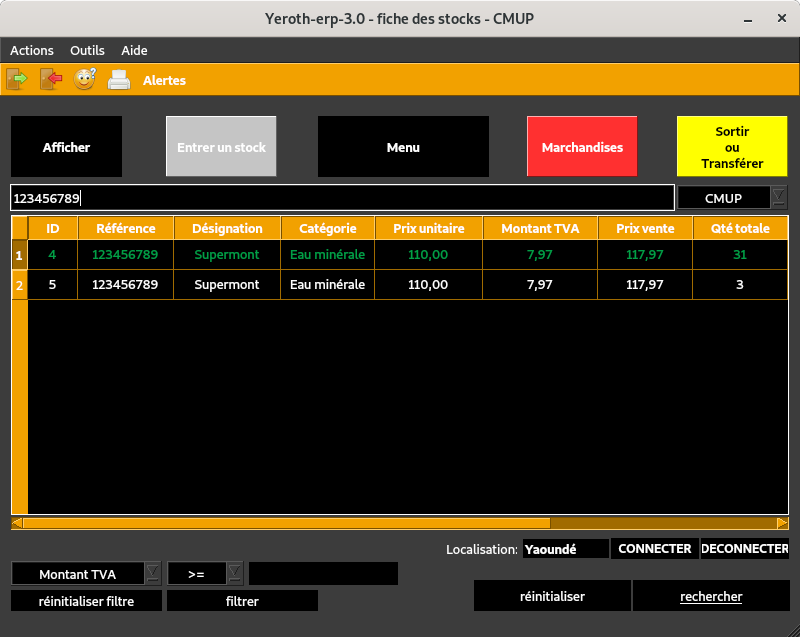
\includegraphics[scale=0.63]{images/yeren-fenetre-rechercher-stock-par-reference.png}
		\caption{Le champs de texte pour
			rechercher les stocks (ou articles) en utilisant
			seulement leur r\'ef\'erence.}\label{fig:yeren-fenetre-rechercher-stock-par-reference}
	\end{figure}
	
	Ceci est illustr\'e dans la figure~\ref{fig:yeren-fenetre-rechercher-stock-par-reference}
	o\`u les stocks ayant la r\'ef\'erence '\textbf{123456789}'
	ont \'et\'e recherch\'es.\\	
\end{itemize}

Lorsqu'une recherche de stocks (ou d'articles) est active,
le mot 'rechercher' du bouton \bouton{rechercher} et
le lien '\textbf{Rechercher un article}' dans le
menu d\'eroulant '\textbf{Outils}' sont soulign\'es.
	
Le bouton \bouton{r\'einitialiser} ou le lien
'\textbf{R\'einitialiser la recherche}' dans le menu 
d\'eroulant '\textbf{Outils}' permettent de d\'eactiver
la recherche et ainsi d'afficher tous les stocks
\`a nouveau.

%-----------------------------------------------------------
\newpage
\nxsection{Afficher les d\'etails d'un stock}
\index{afficher les d\'etails d'un stock}

La figure~\ref{fig:fenetre-details-stock} illustre
les d\'etails du stock '\textbf{Supermont}'.\\

\begin{figure}[!htbp]
	\centering
	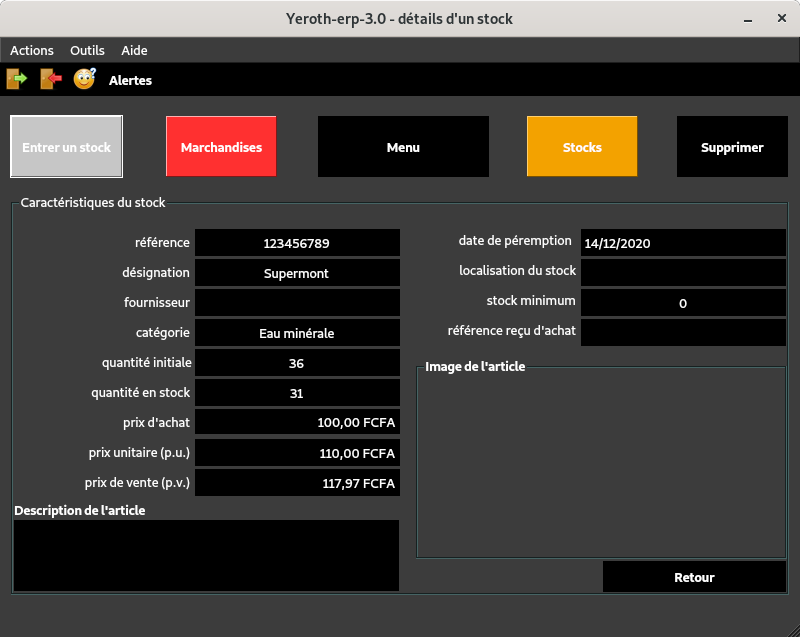
\includegraphics[scale=0.63]{images/yeren-fenetre-detail-stock.png}
	\caption{Une fen\^etre qui pr\'esente les d\'etails d'un stock.}
	\label{fig:fenetre-details-stock}
\end{figure}

Il existe trois m\'ethodes pour afficher les d\'etails
d'un stock:

\begin{itemize}[\mycheckmark{purplish}]
	\item \textcolor{purplish}{$\mathbf{1^{\text{\`ere}}}$ \textbf{m\'ethode}}
		\begin{enumerate}[1)]
			\item s\'electionnez le stock dont vous souhaitez
			afficher les d\'etails en cliquant une fois sur lui
			\` a partir de la fen\^etre '\textbf{fiche des stocks}'
			
			\item cliquez ensuite sur le bouton \bouton{Afficher}.	\\
		\end{enumerate}
	
	\item \textcolor{purplish}{$\mathbf{2^{\text{\`eme}}}$ \textbf{m\'ethode}}
		\begin{enumerate}[1)]
			\item s\'electionner le stock dont vous souhaitez
			afficher les d\'etails en cliquant une fois sur lui
			\` a partir de la fen\^etre '\textbf{fiche des stocks}'
			
			\item cliquer ensuite sur le lien '\textbf{Afficher les d\'etails de ce stock}'
			du menu d\'eroulant \textbf{Actions}.\\
		\end{enumerate}
	
	\item \textcolor{purplish}{$\mathbf{3^{\text{\`eme}}}$ \textbf{m\'ethode}}
		\begin{enumerate}[1)]
			\item s\'electionner le stock dont vous souhaitez
			afficher les d\'etails en cliquant une fois sur lui
			\` a partir de la fen\^etre '\textbf{fiche des stocks}'
			
			\item maintener l'indexeur de la souris sur le stock
				s\'electionner et ensuite cliquer sur le bouton
				droit de la souris
			
			\item un menu d\'eroulant s'affiche, cliquer sur
				le lien '\textbf{Afficher les d\'etails de ce stock}' du
				menu d\'eroulant qui s'est affich\'e. 
		\end{enumerate}
\end{itemize}

%-----------------------------------------------------------
\newpage
\nxsection{Consulter l'historique d'un stock}
\index{consulter l'historique d'un stock}
\index{l'historique d'un stock}

La figure~\ref{fig:fenetre-historique-dun-stock}
illustre l'historique d'un stock.

\begin{figure}[!htbp]
	\centering
	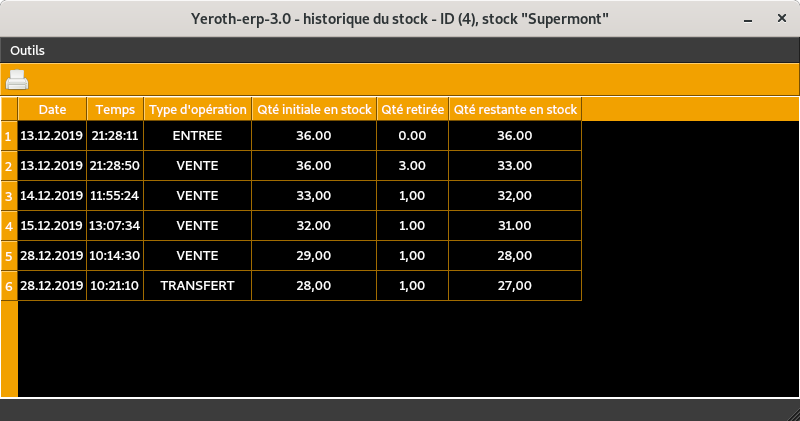
\includegraphics[scale=0.63]{images/yeroth-historique-stock.png}
	\caption{L'historique d'un stock.}
	\label{fig:fenetre-historique-dun-stock}
\end{figure}

\begin{itemize}[\mycheckmark{purplish}]
	\item \textcolor{purplish}{$\mathbf{1^{\text{\`ere}}}$ \textbf{m\'ethode}}
	\begin{enumerate}[1)]
		\item s\'electionner le stock dont vous souhaitez
		consulter l'historique en cliquant sur lui avec
		le boutton gauche de la souris
		\` a partir de la fen\^etre '\textbf{fiche des stocks}'
		
		\item cliquer ensuite sur le lien
		 '\textbf{Afficher l'historique de ce stock}' du
		 menu d\'eroulant \textbf{Actions}.\\
	\end{enumerate}
	
	\item \textcolor{purplish}{$\mathbf{2^{\text{\`eme}}}$ \textbf{m\'ethode}}
	\begin{enumerate}[1)]
		\item s\'electionner le stock dont vous souhaitez
		consulter l'historique en cliquant sur lui avec
		le boutton droit de la souris
		\` a partir de la fen\^etre '\textbf{fiche des stocks}'
		
		\item cliquer ensuite sur le lien
		 '\textbf{Afficher l'historique de ce stock}' du
		 menu contextuel qui s'est affich\'e.\\
	\end{enumerate}
	
\end{itemize}

L'historique du stock peut \^etre imprim\'e
au format PDF en cliquant sur l'ic\^one
repr\'esentant une imprimante.


%-----------------------------------------------------------
\newpage
\nxsection{Modifier les d\'etails d'un stock}
\index{modifier les d\'etails d'un stock}

La figure~\ref{fig:yeren-fenetre-modifier-stock}
illustre la fen\^etre pour modifier les d\'etails
du stock '\textbf{Cola}'.\\

\begin{figure}[!htbp]
	\centering
	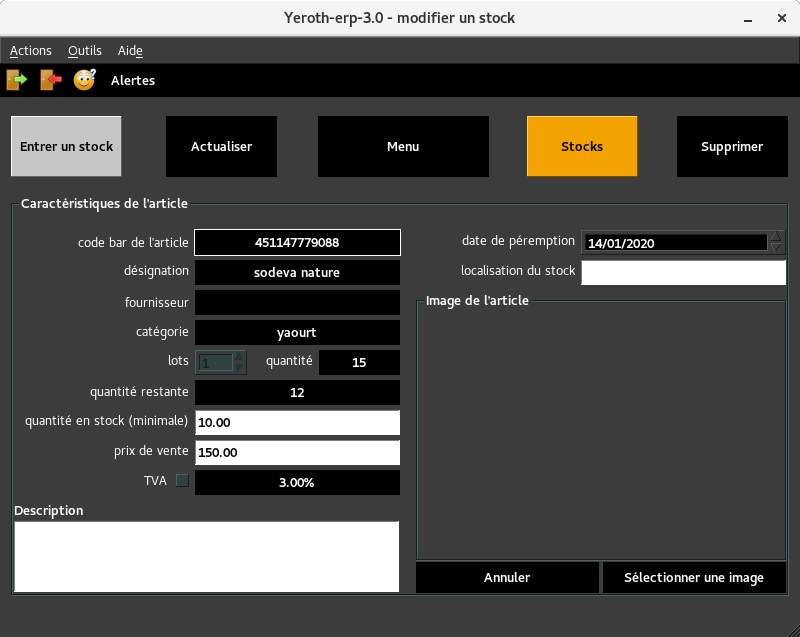
\includegraphics[scale=0.63]{images/yeren-fenetre-modifier-stock.png}
	\caption{Une fen\^etre qui permet la modification des d\'etails d'un stock.}
	\label{fig:yeren-fenetre-modifier-stock}
\end{figure}

Seul les informations suivantes d'un stock peuvent
\^etre modifi\'ees:
\begin{enumerate}[1)]
	\item la date de p\'eremption des articles du stock
	\item la quantit\'e minimale en stock
	\item le prix de vente d'un article du stock.\\
\end{enumerate}

Il existe trois m\'ethodes pour modifier les d\'etails
d'un stock:

\begin{itemize}[\mycheckmark{purplish}]
	\item \textcolor{purplish}{$\mathbf{1^{\text{\`ere}}}$ \textbf{m\'ethode}}
	\begin{enumerate}[1)]
		\item s\'electionner le stock dont vous souhaitez
		modifier les d\'etails en cliquant une fois sur lui
		\` a partir de la fen\^etre '\textbf{fiche des stocks}'
		
		\item cliquer ensuite sur le bouton \bouton{Modifier}.	\\
	\end{enumerate}
	
	\item \textcolor{purplish}{$\mathbf{2^{\text{\`eme}}}$ \textbf{m\'ethode}}
	\begin{enumerate}[1)]
		\item s\'electionner le stock dont vous souhaitez
		modifier les d\'etails en cliquant une fois sur lui
		\` a partir de la fen\^etre '\textbf{fiche des stocks}'
		
		\item cliquer ensuite sur le lien '\textbf{Modifier ce stock}'
		du menu d\'eroulant \textbf{Actions}.\\
	\end{enumerate}
	
	\item \textcolor{purplish}{$\mathbf{3^{\text{\`eme}}}$ \textbf{m\'ethode}}
	\begin{enumerate}[1)]
		\item s\'electionner le stock dont vous souhaitez
		modifier les d\'etails en cliquant une fois sur lui
		\` a partir de la fen\^etre '\textbf{fiche des stocks}'
		
		\item maintener l'indexeur de la souris sur le stock
		s\'electionn\'e et ensuite cliquer sur le bouton
		droit de la souris
		
		\item un menu d\'eroulant s'affiche, cliquer sur
		le lien '\textbf{Modifier ce stock}' du	menu
		d\'eroulant qui s'est affich\'e.\\
	\end{enumerate}
\end{itemize}

%-----------------------------------------------------------

\newpage
\nxsection{Visualiser les articles / stocks p\'erim\'es}
\index{visualiser les articles p\'erim\'es}
\index{visualiser les stocks p\'erim\'es}

La figure~\ref{fig:fenetre-lister-stock-perime} illustre
que la date de p\'eremption du stock 'Cola' ($22$ F\'evrier
$2017$) est d\'epass\'ee.\\

\begin{figure}[!htbp]
	\centering
	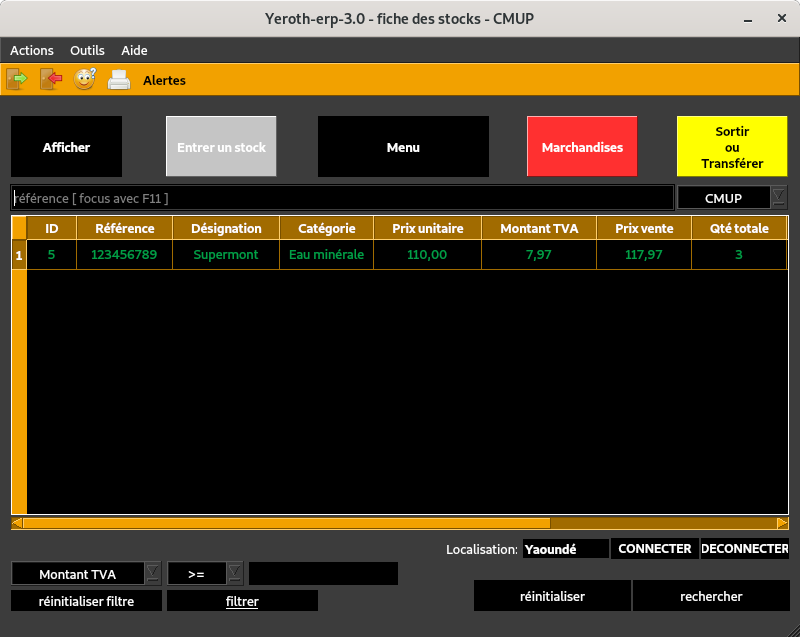
\includegraphics[scale=0.63]{images/yeren-fenetre-stocks-perimes.png}
	\caption{Le stock 'Cola' est p\'erim\'e.}
	\label{fig:fenetre-lister-stock-perime}
\end{figure}

On visualise les stocks p\'erim\'es en allant \`a la fen\^etre
'\textbf{fiche des stocks}'. 

Tous les stocks dont la colone '\textbf{Date de
	p\'eremption}' est affich\'ee en 
\textbf{\textcolor{firebrickred}{rouge}} sont p\'erim\'es.

%-----------------------------------------------------------

\newpage
\nxsection{Visualiser les stocks dont la quantit\'e minimale 
	en stock est atteinte}
\index{la quantit\'e minimale en stock est atteinte}

L'utilisateur de \yeren peut d\'efinir une quantit\'e minimale
pour un stock: c'est \emph{le nombre d'articles du stock en dessous
duquel l'entreprise ne devrait pas se retrouver}.

La figure~\ref{fig:fenetre-lister-quantite-minimale} illustre
que la quantit\'e minimale de $50$ articles du stock 'Cola'
est atteinte.\\

\begin{figure}[!htbp]
	\centering
	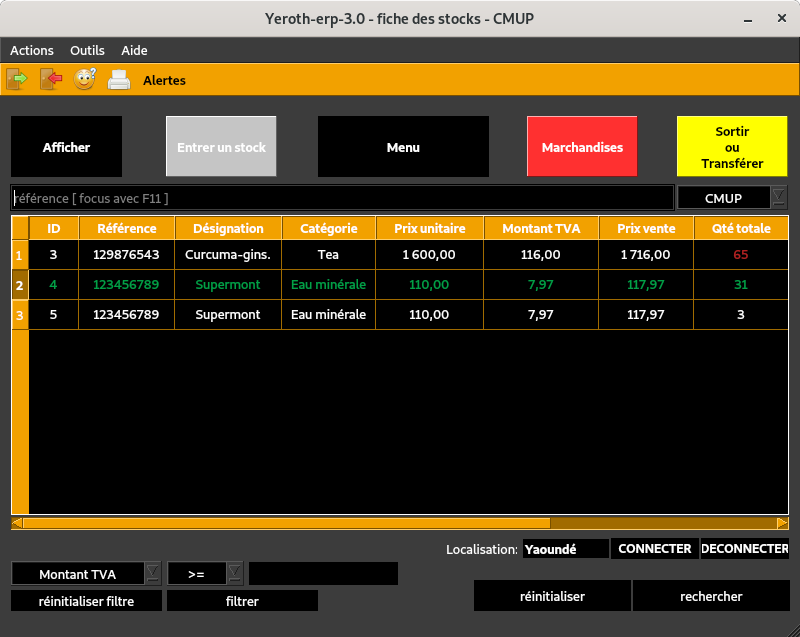
\includegraphics[scale=0.63]{images/yeren-fenetre-stock-minimal-atteint.png}
	\caption{La quantit\'e minimale du stock 'Cola' est atteinte.}
	\label{fig:fenetre-lister-quantite-minimale}
\end{figure}

On visualise les stocks dont la quantit\'e minimale en stock
est atteinte en allant \`a la fen\^etre '\textbf{fiche des stocks}'.

Tous les stocks dont la colone '\textbf{Quantit\'e en stock}'
est affich\'ee en \textbf{\textcolor{firebrickred}{rouge}}
ont leur quantit\'e minimale en stock d\'ej\`a ateinte.

%-----------------------------------------------------------

%\newpage
\nxsection{Supprimer un stock}
\index{supprimer un stock}

Il existe deux m\'etodes pour supprimer un stock:
\begin{itemize}[\mycheckmark{purplish}]
	\item \textcolor{purplish}{$\mathbf{1^{\text{\`ere}}}$ \textbf{m\'ethode}}
	
	\begin{enumerate}[1)]
		\item s\'electionner le stock \`a supprimer partir de
		la fen\^etre '\textbf{fiche des stocks}'
		
		\item cliquer ensuite sur le lien '\textbf{Supprimer ce stock}'
		dans le menu d\'eroulant \textbf{Actions}.\\
	\end{enumerate}
	
	\item \textcolor{purplish}{$\mathbf{2^{\text{\`eme}}}$ \textbf{m\'ethode}}
	\begin{enumerate}[1)]
		\item s\'electionner le stock \`a supprimer partir de
			la fen\^etre '\textbf{fiche des stocks}'
		
		\item maintener l'indexeur de la souris sur le stock
			s\'electionn\'e et ensuite cliquer sur le bouton
			droit de la souris
				
		\item un menu d\'eroulant s'affiche, cliquer sur
			le lien '\textbf{Supprimer ce stock}' du menu
			d\'eroulant qui s'est affich\'e. \\
	\end{enumerate}	
\end{itemize}

Le stock supprim\'e n'est plus affich\'e.

\chapter{La Gestion des Clients}
\label{chap:gestion-des-clients}



\begin{figure}[!htbp]
\centering
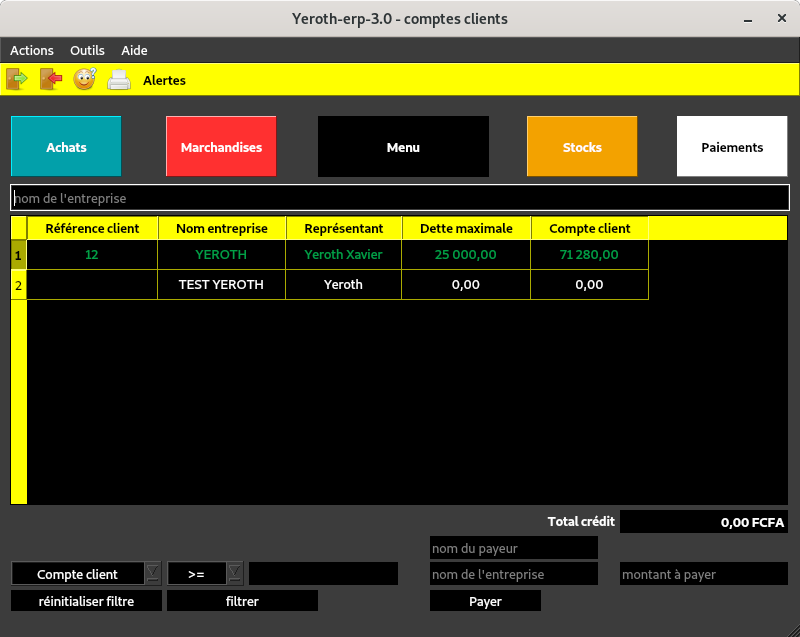
\includegraphics[scale=0.63]{images/yeroth-lister-des-clients.png}
\caption{La fen\^etre pour lister des clients.}
\label{fig:fenetre-lister-des-clients}
\end{figure}
\chapter{La Gestion des Achats}
\label{chap:gestion-des-achats}




\begin{figure}[!htbp]
\centering
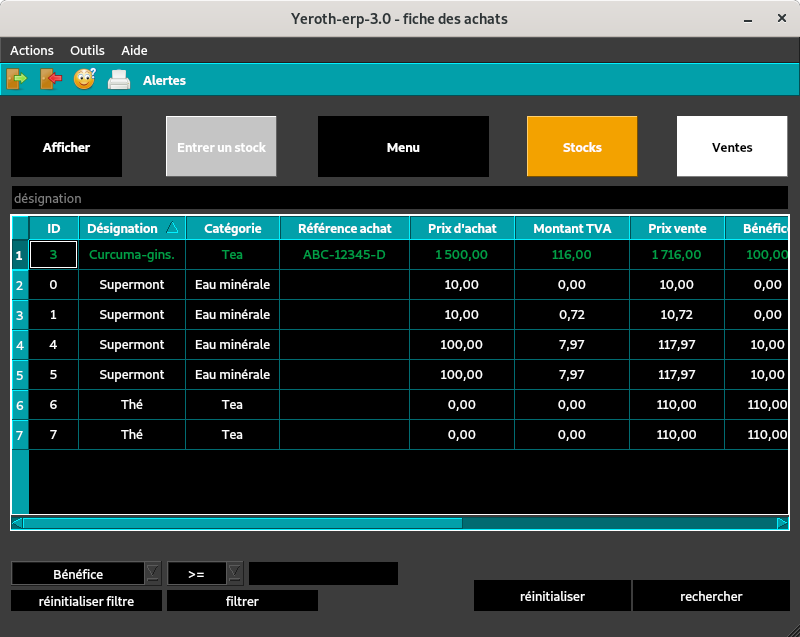
\includegraphics[scale=0.63]{images/yeroth-lister-des-achats.png}
\caption{La fen\^etre pour lister des achats.}
\label{fig:fenetre-lister-des-achats}
\end{figure}
\chapter{Le Syst\`eme d'Alertes sur les Stocks}\label{chap:systeme-dalertes}
\index{syst\`eme d'alertes}

\utilisateurs: \lienadmin, \liencaissier, \lienmagasinier, \lienpatron.\\

\chapintro{Ce chapitre d\'ecrit comment cr\'eer, lister, modifier,
et supprimer les alertes sur les stocks.}

\nxsection{Introduction}

Le programme qui impl\'emente le syst\`eme d'alertes
de \yeren s'appelle ''\emphbf{yeren-alert}''.

\yerenalert est configur\'e pour d\'emarrer en tant que
''\emphbf{processus en arri\`ere plan}'' lors du
d\'emarrage de l'ordinateur.

La figure~\ref{fig:yeren-fenetre-creer-alerte}
pr\'esente l'interface graphique de \yeren pour
cr\'eer une alerte.

\begin{figure}[!htbp]
	\centering
	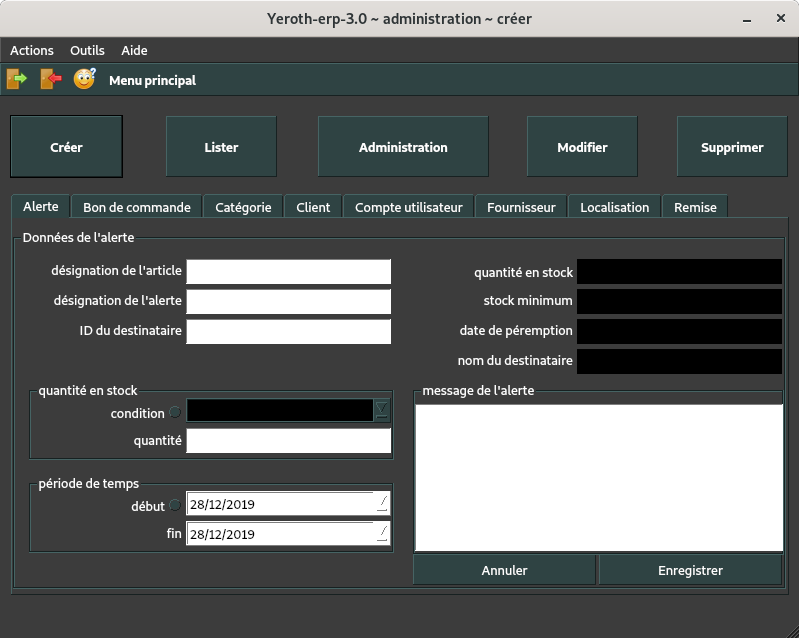
\includegraphics[scale=0.63]{images/yeren-fenetre-creer-alerte.png}
	\caption{La fen\^etre principale pour la cr\'eation d'une alerte.}
	\label{fig:yeren-fenetre-creer-alerte}
\end{figure}

le syst\`eme d'alertes sur les stocks permet aux
utilisateurs de contr\^oler \emph{les dates de
p\'eremption des stocks},
ainsi que \emph{les quantit\'es d'articles en stock}.

\yeren d\'efinit deux types d'alertes sur les stocks:
\begin{enumerate}[1)]
	\item \textbf{les alertes sur une quantit\'e en stock}
	\item \textbf{les alertes sur une p\'eriode de temps}.\\
\end{enumerate}

L'interface de \yeren pour cr\'eer des alertes a deux
\emph{boutons de radio}~\footnote{les boutons de radio
	permettent de faire des choix exclusifs}:

\begin{enumerate}[1)]
	\item le bouton de radio 'quantit\'e en stock'
	\item le bouton de radio 'p\'eriode de temps'.
\end{enumerate}

%-----------------------------------------------------------

\newpage
\nxsection{Cr\'eer une alerte sur une quantit\'e en stock}\label{sec:alerte-quantite-stock}
\index{cr\'eer une alerte sur une quantit\'e en stock}

\begin{enumerate}[1)]
	\item \`A partir de l'interface graphique de l'acceuil de
		l'administration (voir figure~\ref{fig:fenetre-administrateur}),
		on clique sur l'onglet intitul\'e \textbf{op\'erations}. 
		
	\item Choisir '\textbf{cr\'eer}' dans le '\emph{combo box
		op\'erations}'.
		
	\item Choisir '\textbf{une alerte}' dans le '\emph{combo box
		sujets}'. Vous \^etes automatiquement conduit \`a la fen\^etre
		illustr\'ee sur la figure~\ref{fig:yeren-fenetre-creer-alerte}.	
		
	\item Il est pr\'ef\'erable pour de d'abord	choisir le stock
		pour lequel une alerte doit \^etre cr\'eer.	Pour cela il
		faut choisir sa d\'esignation dans le champs de texte
		'\textbf{d\'esignation de l'article}', qui poss\`ede un
		menu auto-d\'eroulant.\\

		Les informations des champs de textes situ\'ees \`a
		droite du champs de texte '\textbf{d\'esignation de l'article}'
		sont non modifiables et affichent des valeurs en fonction
		du stock de l'article s\'electionn\'e:
		\begin{enumerate} [1)]
			\item quantit\'e en stock
			\item quantit\'e minimale (stock)
			\item date de p\'eremption.		
		\end{enumerate}

		Ces informations aident \`a param\'etrer l'alerte.

	\item Donner une d\'esignation \`a l'alerte	en remplissant
		le champs de texte '\textbf{d\'esignation de l'alerte}'.
		
	\item Choisir un destinataire qui recevra le message de
		l'alerte lorsque celle-ci sera d\'eclench\'ee.
		Ceci se fait dans le champs de texte '\textbf{ID du destinataire}',
		qui poss\`ede un menu auto-d\'eroulant.\\
		
		Le nom complet du destinataire est affich\'e automatiquement
		dans le champs de texte '\textbf{nom du destinataire}',
		qui est situ\'e juste \`a droite du champs de texte
		'\textbf{ID du destinataire}'.
		
	\item Choisir le type d'alerte:	\emphbf{quantit\'e en stock}
		en cliquant sur la bouton radio '\textbf{condition}' et 
		en \emph{saisissant un nombre dans le champs de texte
		'\textbf{quantit\'e}'}.
		
	\item Remplir le champs de texte '\textbf{Message de l'alerte}'.
		C'est ce message qui sera envoy\'e au destinataire de
		l'alerte lorsque celle-ci sera d\'eclench\'ee.	
		
	\item Achever la proc\'edure en cliquant sur le bouton \bouton{Valider}.
\end{enumerate}

%-----------------------------------------------------------

\newpage
\nxsection{Cr\'eer une alerte sur une p\'eriode de temps}\label{sec:alerte-periode-temps}
\index{cr\'eer une alerte sur une p\'eriode de temps}

\begin{enumerate}[1)]
	\item \`A partir de l'interface graphique de l'acceuil de
		l'administration (voir figure~\ref{fig:fenetre-administrateur}),
		on clique sur l'onglet intitul\'e \textbf{op\'erations}. 
		
	\item Choisir '\textbf{cr\'eer}' dans le '\emph{combo box
		op\'erations}'.
		
	\item Choisir '\textbf{une alerte}' dans le '\emph{combo box
		sujets}'. Vous \^etes automatiquement conduit \`a la fen\^etre
		illustr\'ee sur la figure~\ref{fig:yeren-fenetre-creer-alerte}.	
		
	\item Il est pr\'ef\'erable pour de d'abord	choisir le stock
		pour lequel une alerte doit \^etre cr\'eer.	Pour cela il
		faut choisir sa d\'esignation dans le champs de texte
		'\textbf{d\'esignation de l'article}', qui poss\`ede un
		menu auto-d\'eroulant.\\

		Les informations des champs de textes situ\'ees \`a
		droite du champs de texte '\textbf{d\'esignation de l'article}'
		sont non modifiables et affichent des valeurs en fonction
		du stock de l'article s\'electionn\'e:
		\begin{enumerate} [1)]
			\item quantit\'e en stock
			\item quantit\'e minimale (stock)
			\item date de p\'eremption.		
		\end{enumerate}

		Ces informations aident \`a param\'etrer l'alerte.

	\item Donner une d\'esignation \`a l'alerte	en remplissant
		le champs de texte '\textbf{d\'esignation de l'alerte}'.
		
	\item Choisir un destinataire qui recevra le message de
		l'alerte lorsque celle-ci sera d\'eclench\'ee.
		Ceci se fait dans le champs de texte '\textbf{ID du destinataire}',
		qui poss\`ede un menu auto-d\'eroulant.\\
		
		Le nom complet du destinataire est affich\'e automatiquement
		dans le champs de texte '\textbf{nom du destinataire}',
		qui est situ\'e juste \`a droite du champs de texte
		'\textbf{ID du destinataire}'.
		
	\item Choisir le type d'alerte:	\emphbf{p\'eriode de temps}
		en cliquant sur la bouton radio '\textbf{d\'ebut}' et 
		en choisissant \emph{les dates de d\'ebut et de fin de
		la p\'eriode de temps pendant laquelle l'alerte sera active}.
		
	\item Remplir le champs de texte '\textbf{Message de l'alerte}'.
		C'est ce message qui sera envoy\'e au destinataire de
		l'alerte lorsque celle-ci sera d\'eclench\'ee.	
		
	\item Achever la proc\'edure en cliquant sur le bouton \bouton{Valider}.
\end{enumerate}

%-----------------------------------------------------------

\newpage
\nxsection{Voir toutes les alertes qu'un utilisateur
 a re\c{c}u~\textcolor{blue}{*}}\label{sec:voire-toutes-alertes}
\index{voir toutes les alertes qu'un utilisateur a re\c{c}u }

\textcolor{blue}{*: Cette fonctionalit\'e est exclusivement
	r\'eserv\'ee aux utilisateurs \patron.}

Pour voire toutes les alertes qui lui sont destin\'ees, l'utilisateur
doit accomplir les actions suivantes \`a partir de toutes fen\^etre
ayant le lien '\textbf{Alertes}' dans sa barre de menu:
\begin{enumerate}[1)]
	\item cliquer sur le lien '\textbf{Alertes}' qui est situ\'e
	dans la barre de menu. Ce lien se retrouve dans toutes les
	fen\^etres concernant la gestion des stocks
	
	\item un utilisateur a aussi acc\`es aux alertes qui lui sont destin\'ees en cliquant sur le lien '\textbf{Alertes}' que
	l'on retrouve dans le menu d\'eroulant \textbf{Outils}.
\end{enumerate}

%-----------------------------------------------------------

\nxsection{Voir les d\'etails d'une alerte}\label{sec:voire-details-alerte}
\index{voir les d\'etails d'une alerte}

L'utilisateur doit accomplir les actions suivantes \`a
partir de toutes fen\^etre ayant le lien '\textbf{Alertes}'
dans sa barre de menu:

\begin{enumerate}[1)]
	\item cliquer sur le lien '\textbf{Alertes}' qui est situ\'e
	dans la barre de menu. Ce lien se retrouve dans toutes les
	fen\^etres concernant la gestion des stocks
		
	\item ensuite, s\'electioner dans l'onglet '\textbf{Alertes}'
		l'alerte dont vous souhaiter voire les d\'etails

	\item enfin, cliquer 2 fois cons\'ecutives sur cette alerte.	
\end{enumerate}

%-----------------------------------------------------------

\nxsection{Marquer une alerte comme r\'esolue~\textcolor{blue}{*}}
\index{marquer une alerte comme r\'esolue}

\textcolor{blue}{*: Cette fonctionalit\'e est exclusivement
	r\'eserv\'ee aux utilisateurs \patron.}

L'utilisateur doit accomplir les actions suivantes \`a
partir de toutes fen\^etre ayant le lien '\textbf{Alertes}'
dans sa barre de menu:

\begin{enumerate}[1)]
	\item cliquer sur le lien '\textbf{Alertes}' qui est situ\'e
	dans la barre de menu. Ce lien se retrouve dans toutes les
	fen\^etres concernant la gestion des stocks
		
	\item ensuite, s\'electioner dans l'onglet '\textbf{Alertes}'
		l'alerte dont vous souhaiter voire les d\'etails

	\item enfin, cliquez sur le bouton \bouton{Marquer r\'esolue}.	
\end{enumerate}

%-----------------------------------------------------------
\newpage
\nxsection{Supprimer une alerte~\textcolor{blue}{*}}
\index{supprimer une alerte}

\textcolor{blue}{*: Cette fonctionalit\'e est exclusivement
		r\'eserv\'ee aux utilisateurs \patron.}

L'utilisateur doit accomplir les actions suivantes \`a
partir de toutes fen\^etre ayant le lien '\textbf{Alertes}'
dans sa barre de menu:

\begin{enumerate}[1)]
	\item cliquer sur le lien '\textbf{Alertes}' qui est situ\'e
	dans la barre de menu. Ce lien se retrouve dans toutes les
	fen\^etres concernant la gestion des stocks
		
	\item ensuite, s\'electioner dans l'onglet '\textbf{Alertes}'
		l'alerte dont vous souhaiter voire les d\'etails

	\item enfin, cliquez sur le bouton \bouton{Supprimer une alerte}.
\end{enumerate}

\chapter{Point De Vente (La Vente d'Articles)}\label{chap:vendre}
\index{vendre des articles}
\index{vendre des stocks}

\utilisateurs: \liencaissier, \lienmanager.\\

\chapintro{Ce chapitre d\'ecrit comment vendre des articles,
appliquer des rabais, et appliquer la TVA sur un
article ou la retirer.}

\nxsection{Introduction}\label{sec:vendre-introduction}

La figure~\ref{fig:fenetre-vendre} illustre
l'interface graphique pour proc\'eder \`a la
vente d'articles.

\begin{figure}[!htbp]
	\centering
	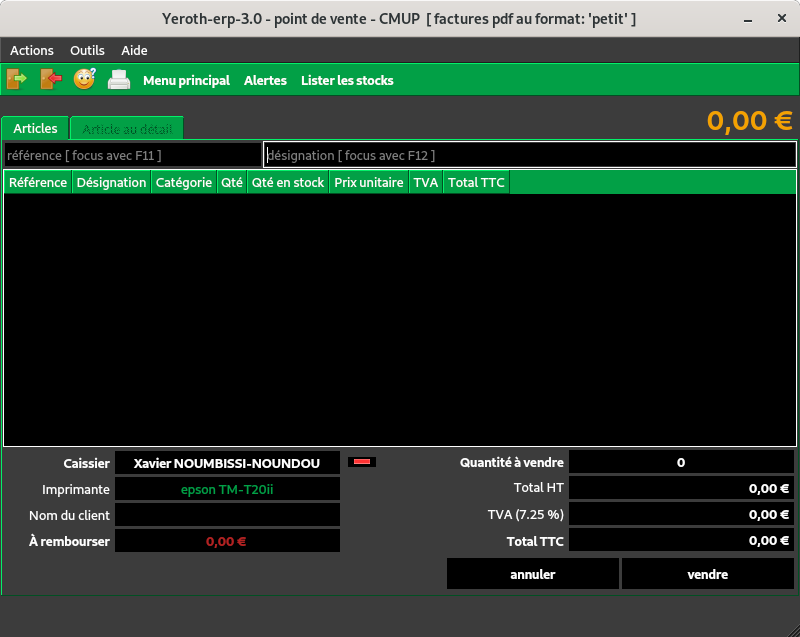
\includegraphics[scale=0.63]{images/yeren-fenetre-caissier.png}
	\caption{La fen\^etre pour vendre les articles.}
	\label{fig:fenetre-vendre}
\end{figure}

Le tableau o\`u sont affich\'es les articles \`a vendre
a les colones suivantes:
\begin{enumerate}[1)]
	\item R\'ef\'erence
	\item D\'esignation
	\item P.U. (\textbf{Prix Unitaire})
	\item Qt\'e (\textbf{Quantit\'e})
	\item Qt\'e restante en stock (\textbf{Quantit\'e restante en stock})
	\item Total TTC (\textbf{Total Toute Taxes Comprise})	
	\item TVA (\textbf{Taxe sur la Valeur Ajout\'e}).
\end{enumerate}

\subsection{La strat\'egie de vente utilis\'ee}
\index{La strat\'egie de vente des articles}
\index{La strat\'egie de vente des stocks}

Le titre de la fen\^etre affiche la strat\'egie de vente
des stocks utilis\'ee. Dans la figure~\ref{fig:fenetre-vendre}
par exemple, la strat\'egie de vente utilis\'ee est
\cmup.

\newpage
%-----------------------------------------------------------

\nxsection{S\'electionner des articles
	\`a vendre}\label{sec:selectionner-articles-vendre}
\index{s\'electionner des articles \`a vendre}
\index{s\'electionner des stocks \`a vendre}

Il existe $2$ m\'ethodes pour s\'electionner des articles
\`a vendre:
\begin{itemize}[\mycheckmark{purplish}]
	\item \textcolor{purplish}{$\mathbf{1^{\text{\`ere}}}$ \textbf{m\'ethode}}\\
	S\'electionner les stocks des articles \`a vendre
	en entrant leur code bar dans le premier champs de texte
	de l'interface (voir figure~\ref{fig:yeren-vendre-choisir-stock-codebar})
	\begin{figure}[!htbp]
		\centering
		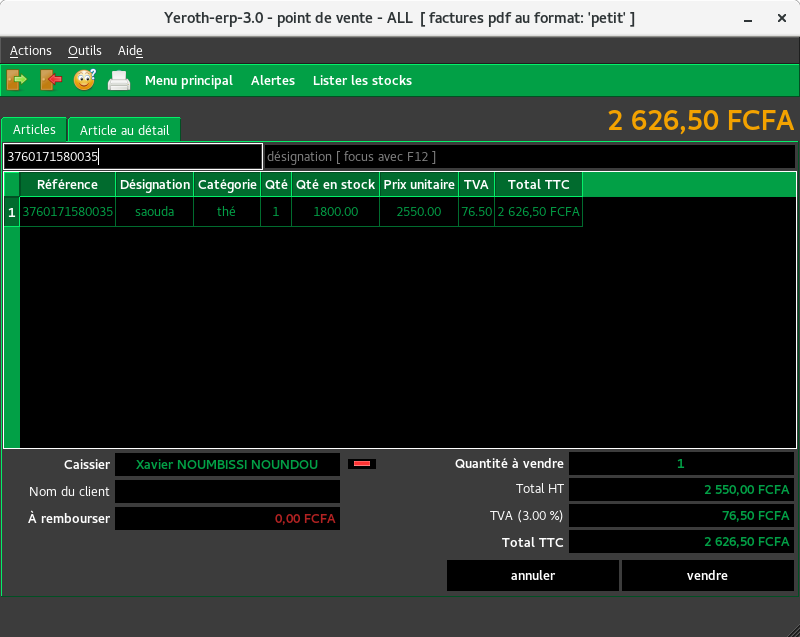
\includegraphics[scale=0.63]{images/yeren-vendre-choisir-stock-codebar.png}
		\caption{Le champs de texte pour
			ajouter les articles en utilisant leur code bar.}\label{fig:yeren-vendre-choisir-stock-codebar}
	\end{figure}
	
	\newpage
	\item \textcolor{purplish}{$\mathbf{2^{\text{\`eme}}}$ \textbf{m\'ethode}}\\
	S\'electionner les stocks des articles \`a vendre
	en entrant leur d\'esignation dans le deuxi\`eme
	champs de texte de l'interface
	(voir figure~\ref{fig:yeren-vendre-choisir-stock-designation}).
	\begin{figure}[!htbp]
		\centering
		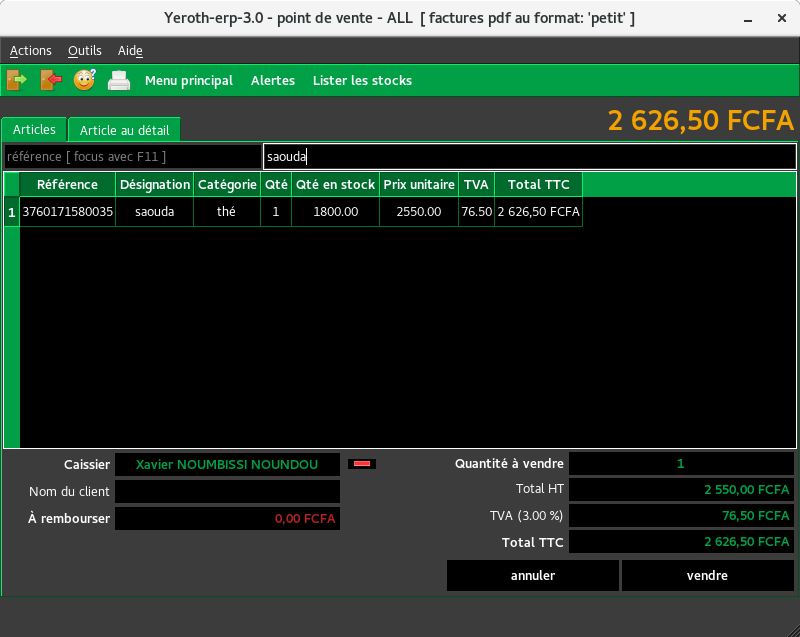
\includegraphics[scale=0.63]{images/yeren-vendre-choisir-stock-designation.png}
		\caption{Le champs de texte pour
			ajouter les articles en utilisant leur d\'esignation.}\label{fig:yeren-vendre-choisir-stock-designation}
	\end{figure}
\end{itemize}

\newpage

%----------------------------------------------------------- 

\nxsection{Afficher les d\'etails d'un article / stock
			s\'electionn\'e pour la vente}
\index{afficher les d\'etails d'un article \`a vendre}
\index{afficher les d\'etails d'un stock \`a vendre}

La figure~\ref{fig:yeren-vente-afficher-details-stock}
illustre les d\'etails du stock 'Saouda'.

Il existe deux m\'etodes pour voir les d\'etails
d'un stock s\'electionn\'e pour la vente:
\begin{itemize}[\mycheckmark{purplish}]
	\item \textcolor{purplish}{$\mathbf{1^{\text{\`ere}}}$ \textbf{m\'ethode}}\\
	Il suffit de cliquer deux fois sur n'importe quelle
	partie autre que '\textbf{Qt\'e}' de la ligne du
	stock s\'electionn\'e.\\
	
	\item \textcolor{purplish}{$\mathbf{2^{\text{\`eme}}}$ \textbf{m\'ethode}}\\
	Il suffit de cliquer sur l'onglet '\textbf{Article au d\'etail}'
	apr\`es la s\'election du stock.
\end{itemize}

%-----------------------------------------------------------
\newpage
\nxsection{Changer la quantit\'e \`a vendre
			d'un article / stock}\label{sec:changer-qte-vendre}
\index{changer la quantit\'e d'un article \`a vendre}
\index{changer la quantit\'e d'un stock \`a vendre}

Il existe deux m\'etodes pour changer la quantit\'e
d'articles d'un stock:
\begin{itemize}[\mycheckmark{purplish}]
	\item \textcolor{purplish}{$\mathbf{1^{\text{\`ere}}}$ \textbf{m\'ethode}}\\
	il faut cliquer sur l'\'el\'ement '\textbf{Qt\'e}'
	avec le bouton gauche de la souris, et ensuite changer la
	quantit\'e \`a vendre (voir figure~\ref{fig:yeren-vendre-qte-selectionner})
	\begin{figure}[!htbp]
		\centering
		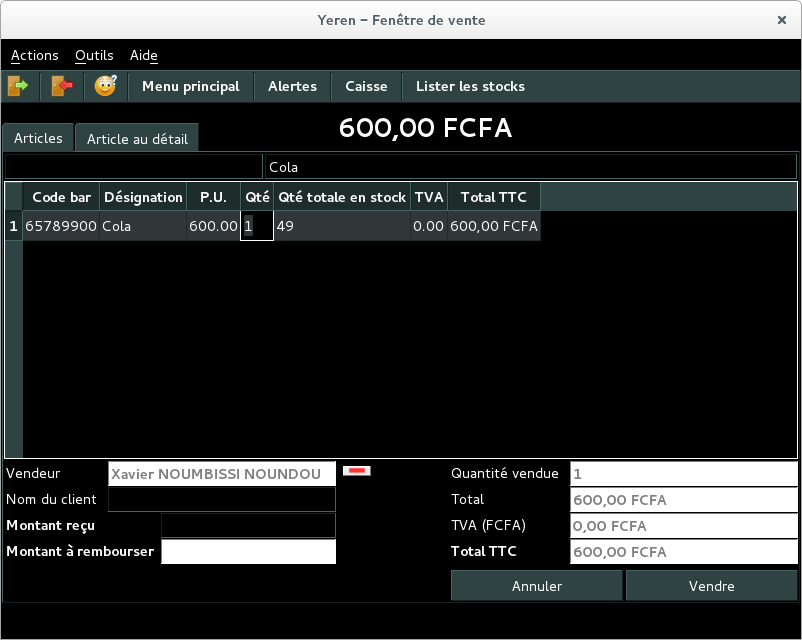
\includegraphics[scale=0.63]{images/yeren-vendre-qte-selectionner.png}
		\caption{L'\'el\'ement 'Qt\'e' s\'electionn\'e pour
			changer la quantit\'e d'articles 'Cola' \`a vendre.}\label{fig:yeren-vendre-qte-selectionner}
	\end{figure}
	\newpage
	
	\item \textcolor{purplish}{$\mathbf{2^{\text{\`eme}}}$ \textbf{m\'ethode}}\\
	il faut cliquer deux fois sur n'importe quel autre
	partie de la ligne du stock s\'electionn\'e, autre que 'Qt\'e'
	pour avoir acc\`es \`a une vue d\'etaill\'ee de ce stock.\\
	
	La vue de d\'etails du stock permet de changer
	la quantit\'e \`a vendre dans le champ de texte
	'\textbf{quantit\'e \`a vendre}'
	(voir figure~\ref{fig:yeren-vente-afficher-details-stock}).
	\begin{figure}[!htbp]
		\centering
		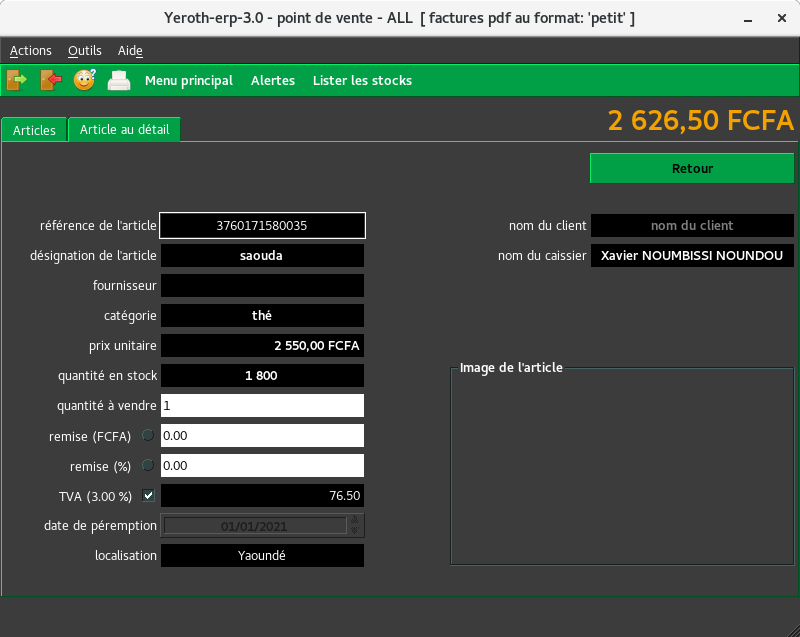
\includegraphics[scale=0.63]{images/yeren-vente-afficher-details-stock.png}
		\caption{Le champs de texte 'quantit\'e \`a vendre'
			permet de changer la quantit\'e \`a vendre d'un article.}
			\label{fig:yeren-vente-afficher-details-stock}
	\end{figure}
\end{itemize}

%-----------------------------------------------------------

\newpage
\nxsection{Appliquer une remise sur
			un article / stock \`a vendre}\label{sec:appliquer-remise-sur-article}
\index{appliquer un rabais sur un article}
\index{appliquer une remise sur un article}
\index{appliquer un rabais sur un stock}
\index{appliquer une remise sur un stock}

Voici la d\'emarche \`a suivre pour appliquer une remise
sur le prix unitaire d'un article \`a vendre:

\begin{enumerate}[1)]
	\item S\'electionner l'article \`a vendre (voir section~\ref{sec:selectionner-articles-vendre})
	\item ouvrer la vue de d\'etails de l'article auquel
		vous souhaitez appliquer une remise
		
	\item appliquer la remise en FCFA ou en pourcentage,
		en choisissant respectivement les bouton de radio
		\bouton{remise (FCFA)} ou \bouton{remise (\%)}, et
		en entrant le montant ou le pourcentage de remise
		\`a appliquer. (voir figure~\ref{fig:yeren-vente-afficher-details-stock})
		
	\item vous pouvez ensuite conclure la vente (voir section~\ref{sec:conclure-une-vente}).
\end{enumerate} 

%-----------------------------------------------------------

\nxsection{Modifier la TVA sur un article \`a vendre}\label{sec:modifier-TVA-article}
\index{ajouter la TVA sur le co\^ut d'un article}
\index{supprimer la TVA sur co\^ut d'un article}

Voici la d\'emarche \`a suivre pour retirer ou ajouter
la TVA sur un article \`a vendre:

\begin{enumerate}[1)]
	\item S\'electionner l'article \`a vendre (voir section~\ref{sec:selectionner-articles-vendre})
	\item ouvrer la vue de d\'etails de l'article auquel
	vous souhaitez appliquer une remise
	
	\item retirer ou ajouter la TVA en cochant le 'check box'
	TVA (voir figure~\ref{fig:yeren-vente-afficher-details-stock}).
	
	\item vous pouvez ensuite conclure la vente (voir section~\ref{sec:conclure-une-vente}).
\end{enumerate} 

%-----------------------------------------------------------
\newpage
\nxsection{Supprimer un article de la liste des articles \`a vendre}
\index{supprimer un article de la liste des articles \`a vendre}

\begin{figure}[!htbp]
	\centering
	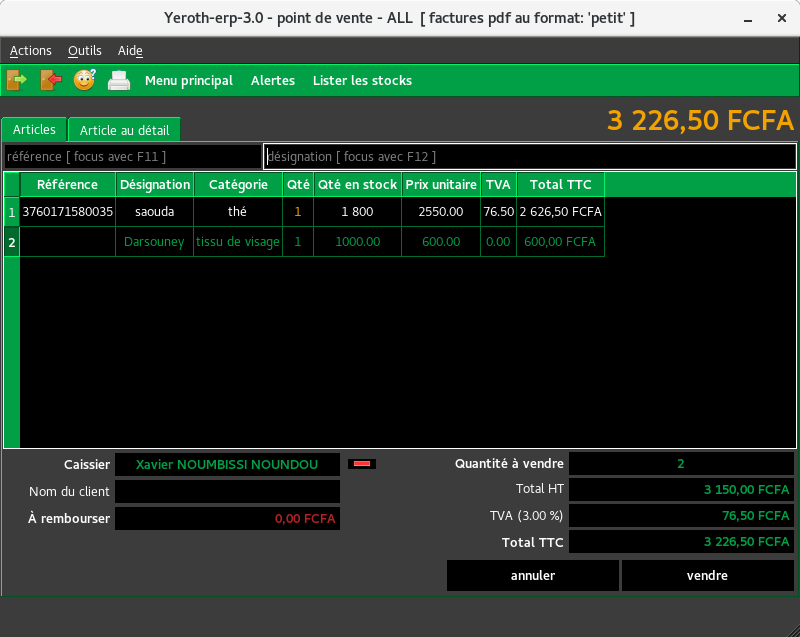
\includegraphics[scale=0.63]{images/yeren-vendre-supprimer-article.png}
	\caption{Le bouton rouge sert \`a supprimer un article
		de la liste des articles \`a vendre.}
	\label{fig:yeren-vendre-supprimer-article}
\end{figure}

Il suffit de s\'electionner la ligne de l'article \`a vendre,
et ensuite cliquer sur le petit bouton rouge qui se trouve
juste apr\`es le champs de texte '\textbf{Caissier}'.

Ce bouton rouge est illustr\'e dans la figure~\ref{fig:yeren-vendre-supprimer-article},
juste apr\`es le champs de texte '\textbf{Caissier}'.
	
%-----------------------------------------------------------
\newpage
\nxsection{Vendre \`a un client divers}\label{sec:vendre-client-divers}
\index{vendre \`a un client divers}

Il suffit de laisser le champs de texte '\textbf{Nom du client}'
vide lors de la vente.

%-----------------------------------------------------------

\nxsection{Vendre \`a un client nomm\'e}\label{sec:vendre-client-nomme}
\index{vendre \`a un client nomm\'e}

Il suffit de saisir le nom du client dans le champs de
texte '\textbf{Nom du client}'.

\begin{figure}[!htbp]
	\centering
	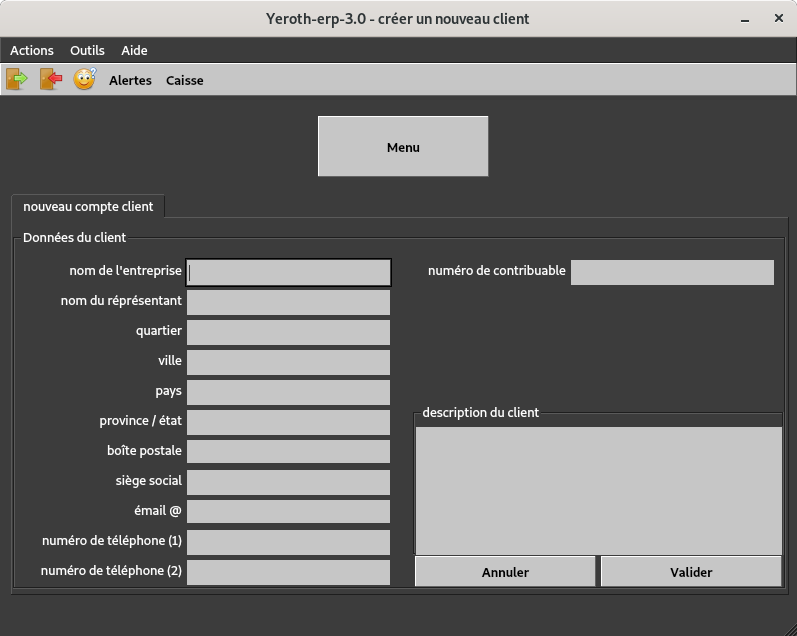
\includegraphics[scale=0.63]{images/yeren-vente-creer-nouveau-client.png}
	\caption{La fen\^etre de la cr\'eation d'un nouveau compte
		client \`a partir de l'interface de vente.}
	\label{fig:yeren-vente-creer-nouveau-client}
\end{figure}

Si le nom du client n'appara\^it pas dans la liste
sugg\'er\'ee, l'utilisateur doit s\'electionner le texte
'\textbf{nouveau client (*)}' (dans la liste sugg\'er'ee).
L'utilisateur sera alors conduit \`a la fen\^etre
pour cr\'eer un nouveau compte client
(figure~\ref{fig:yeren-vente-creer-nouveau-client}).

%-----------------------------------------------------------

\nxsection{Annuler une vente en cours}
\index{annuler une vente en cours}

Il suffit de cliquer sur le bouton \bouton{Annuler} pour annuler
une vente en cours.

%-----------------------------------------------------------

\nxsection{Conclure une vente}\label{sec:conclure-une-vente}
\index{conclure une vente}

Voici la d\'emarche \`a suivre pour conclure une vente:

\begin{enumerate}[1)]
	\item s\'electionner les articles \`a vendre
	(voir section~\ref{sec:selectionner-articles-vendre})
	
	\item entrer les quantit\'es \`a vendre 
	(voir section~\ref{sec:changer-qte-vendre})
	
	\item s'il y'a lieu, appliquer des remises ou modifier
	la TVA (voir section~\ref{sec:appliquer-remise-sur-article})
	
	\item enfin, retourner \`a la fen\^etre titr\'ee
	'\textbf{Yeroth-erp-3.0 - Fen\^etre de la vente'} et
	presser sur le bouton \bouton{Vendre}
	(voir figure~\ref{fig:yeren-vendre-supprimer-article}).
\end{enumerate}

%-----------------------------------------------------------
\nxsection{Imprimer la facture \`a la suite d'une vente}
\index{imprimer la facture \`a la suite d'une vente}
\index{un exemple de facture}

\begin{figure}[!htbp]
	\centering
	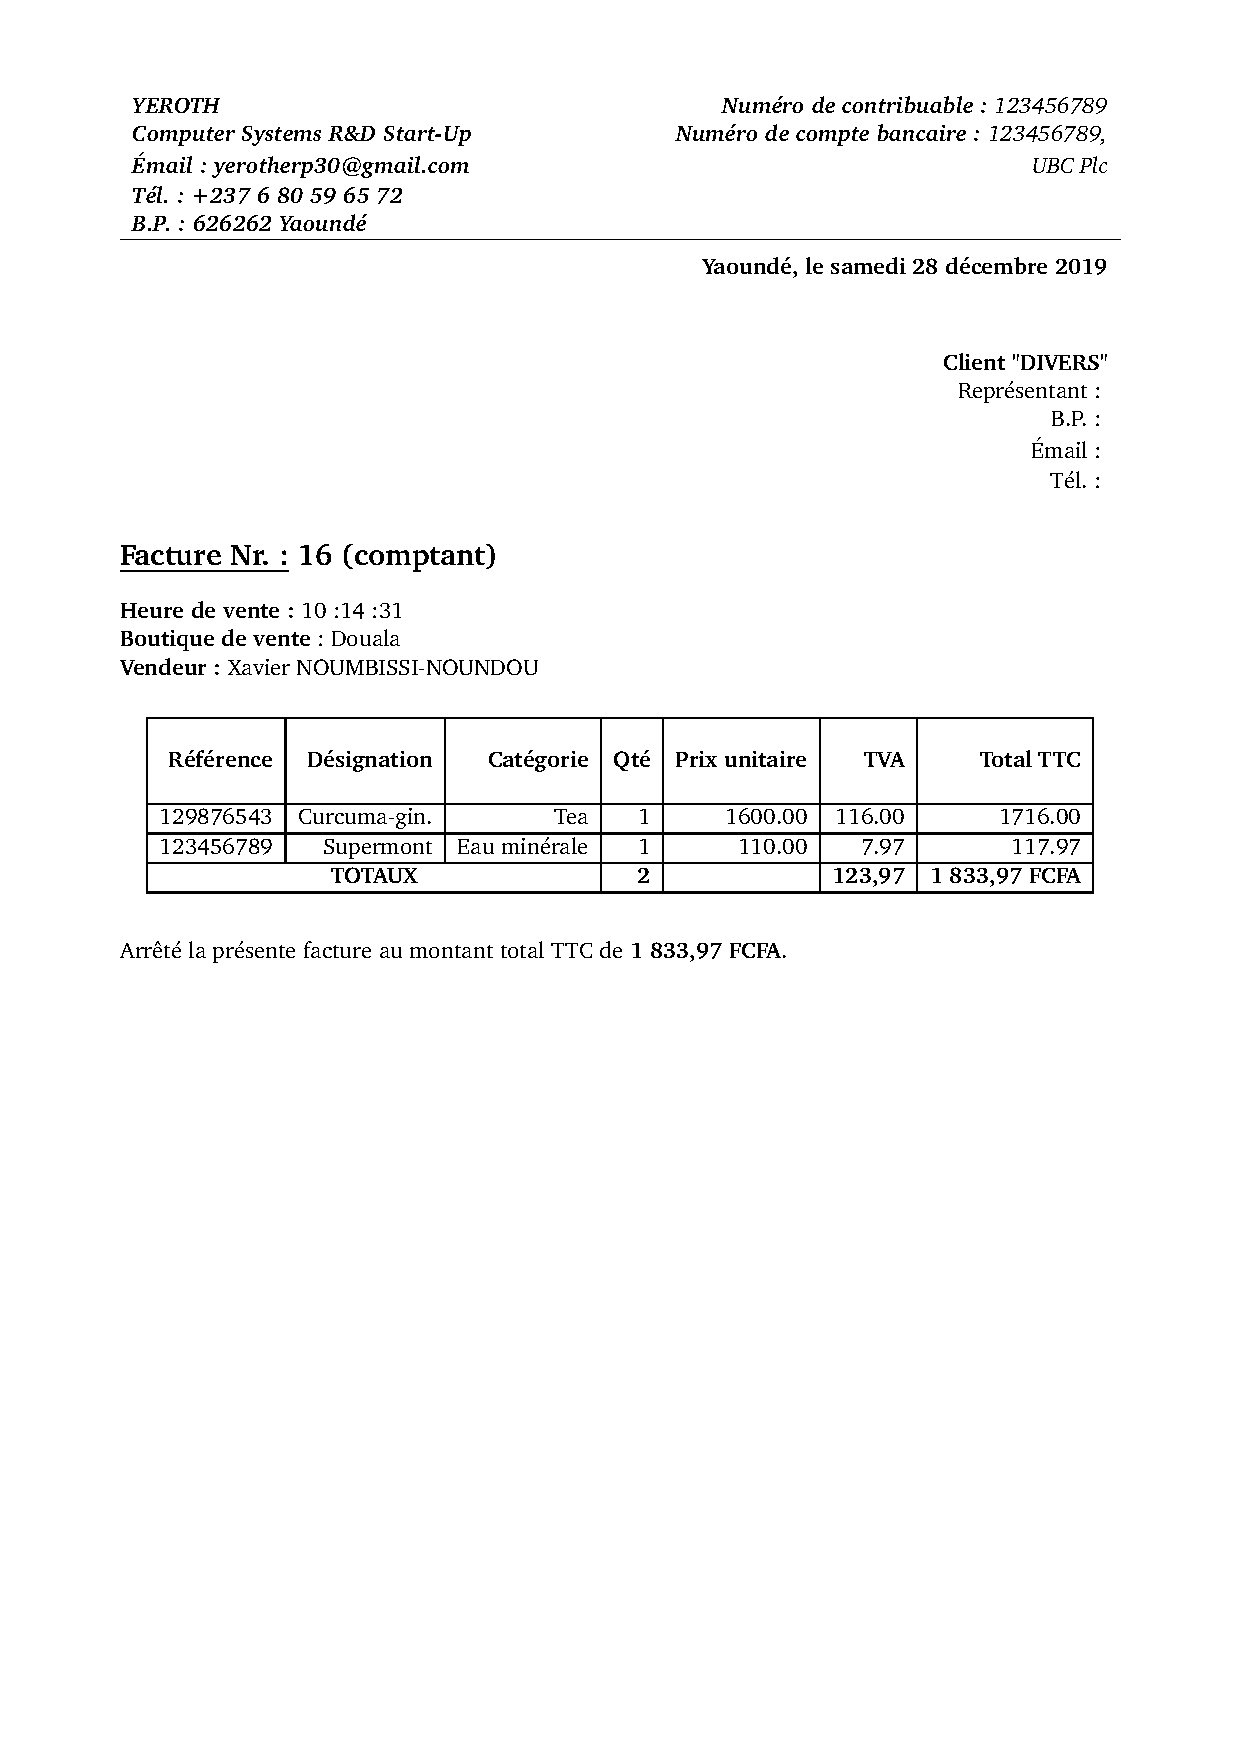
\includegraphics[scale=0.75]{images/yeren-facture-grand-2017-06-13.pdf}
	\caption{Une facture g\'en\'er\'ee \`a la suite d'une vente.}
	\label{fig:yeren-vendre-facture}
\end{figure}

Une facture au format PDF est automatiquement
g\'en\'erer, juste apr\`es qu'une vente soit effectu\'ee.
La figure~\ref{fig:yeren-vendre-facture} illustre un
exemple de facture.

%----------------------------------------------------------- 

\nxsection{Imprimer un exemple de facture au format
	PDF avant de conclure une vente}
\index{un exemple de facture au format PDF}
\index{imprimer un exemple de facture au format PDF}

\begin{figure}[!htbp]
	\centering
	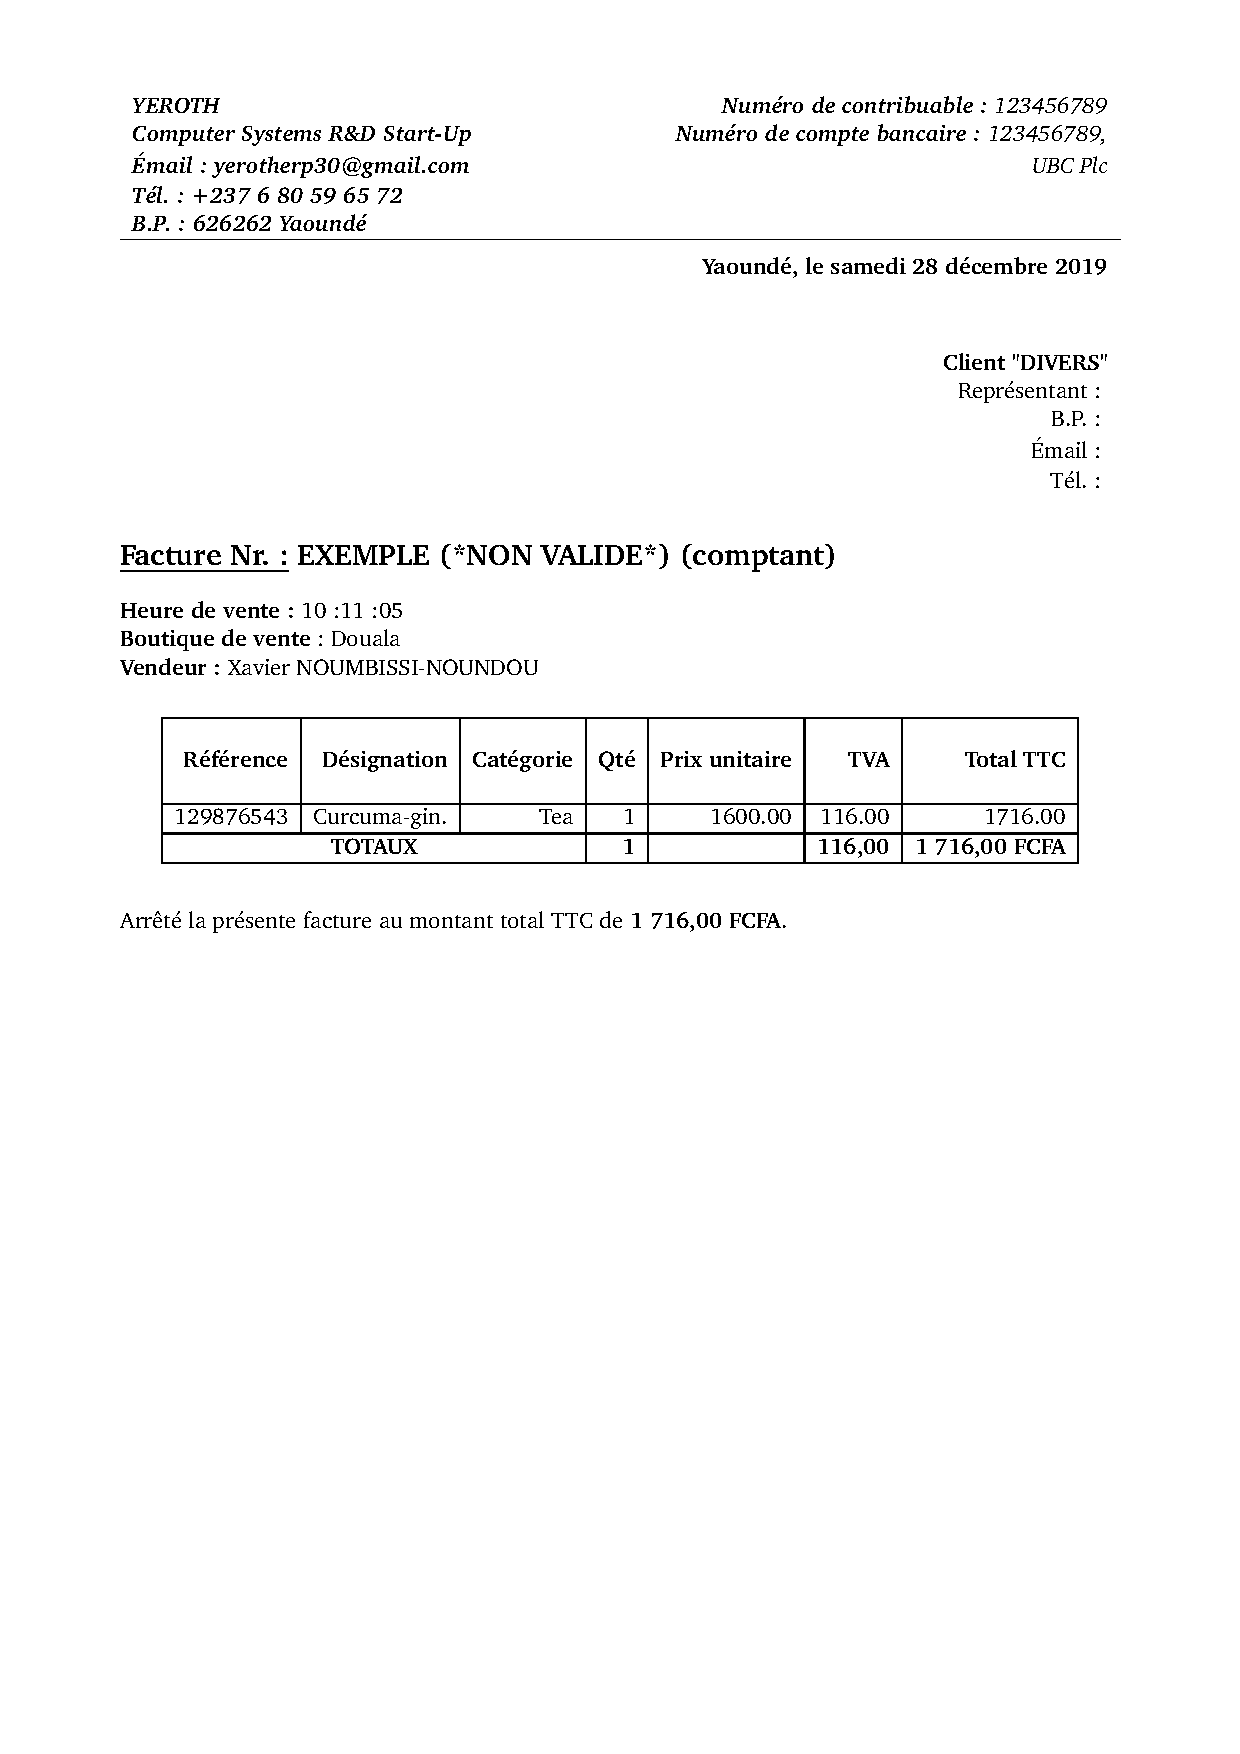
\includegraphics[scale=0.75]{images/yeren-exemple-facture-grand-2017-06-13.pdf}
	\caption{Une facture proforma g\'en\'er\'ee avant de conclure une vente.}
	\label{fig:yeren-vendre-facture-proforma}
\end{figure}

Il existe deux m\'ethodes pour imprimer une facture
proforma avant de conclure la vente \'eventuelle des articles
pr\'esents dans le tableau qui appara\^it dans la fen\^etre
titr\'ee '\textbf{Yeroth-erp-3.0 - Fen\^etre de la vente}'.

\begin{itemize}[\mycheckmark{purplish}]
	\item \textcolor{purplish}{$\mathbf{1^{\text{\`ere}}}$ \textbf{m\'ethode}}\\
		Cliquer sur le lien '\textbf{Imprimer la facture (proforma)}'
		qui se trouve dans le menu d\'eroulant '\textbf{Outils}'\\

	\item \textcolor{purplish}{$\mathbf{2^{\text{\`eme}}}$ \textbf{m\'ethode}}\\
		Presser simultan\'ement les boutons \bouton{CTRL}
		et \bouton{P} de votre clavier.
\end{itemize}

Une facture proforma au format PDF est alors g\'en\'er\'ee. Un
exemple de facture proforma est illustr\'e dans la
figure~\ref{fig:yeren-vendre-facture-proforma}.

\chapter{La Sortie d'Articles}\label{chap:sortir-articles}
\index{la sortie d'articles}
\index{la sortie de stocks}

\utilisateurs: \lienmagasinier, \lienpatron.\\

\chapintro{Ce chapitre d\'ecrit comment proc\'eder \`a la
sortie ou au transfert d'articles.}

\nxsection{Introduction}

\begin{figure}[!htbp]
	\centering
	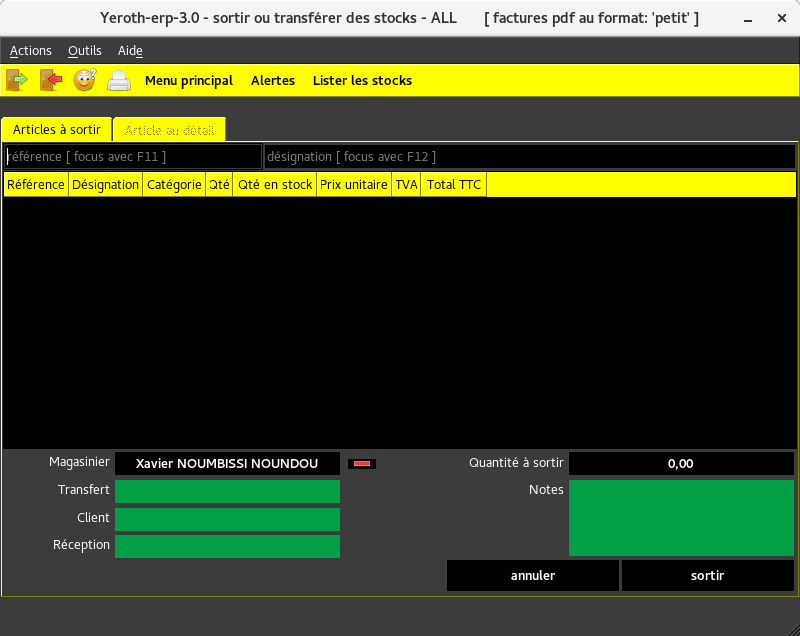
\includegraphics[scale=0.63]{images/yeren-fenetre-sortir-articles.png}
	\caption{La fen\^etre pour sortir des articles en stock.}
	\label{fig:yeren-fenetre-sortir-articles}
\end{figure}

La figure~\ref{fig:yeren-fenetre-sortir-articles} illustre
l'interface graphique pour proc\'eder aux sorties, ou aux
transferts d'articles.

La fen\^etre avec pour titre ''sortir ou transf\'erer des stocks''
permet d'effectuer les op\'erations suivantes:
\begin{enumerate}[1)]
	\item \textbf{une sortie de stocks};
	\item \textbf{un transfert de stocks}.\\
\end{enumerate}

Une \textbf{sortie de stocks} est le retrait d'articles
par un client aupr\`es d'une boutique (ou d'un d\'ep\^ot)
de votre entreprise apr\`es que le paiement se soit
effectu\'e dans une autre unit\'e de l'entreprise.

Un \textbf{transfert de stocks} est un mouvement de stocks
d'une boutique (ou d'un d\'ep\^ot) de votre entreprise
vers une autre unit\'e de l'entreprise.

\subsection{La strat\'egie de sortie des articles / stocks utilis\'ee}
\index{La strat\'egie de sortie des articles}
\index{La strat\'egie de sortie des stocks}

Le titre de la fen\^etre affiche la strat\'egie de sortie
des stocks utilis\'ee. La strat\'egie affich\'ee dans la
figure~\ref{fig:yeren-fenetre-sortir-articles} est: ''\cmup''
(en effet: \textbf{Cours Moyen Unit\'e Pond\'er\'e}).

%---------------------------------------------------

\nxsection{Effectuer une sortie d'articles}
\index{effectuer une sortie d'articles}
\index{effectuer une sortie de stock}

La d\'emarche pour effectuer une sortie d'articles en stock
est la suivante:
\begin{enumerate}[1)]
	\item s\'electionner les articles \`a faire sortir
	(appliquer l'une des m\'ethodes d\'ecrites dans
	la section~\ref{sec:selectionner-articles-vendre}
	du chapitre~\ref{chap:vendre} sur la vente d'article)

	\item le cas \'ech\'eant, choisissez le nom de
	l'entreprise cliente dans le menu d\'eroulant
	du champs de texte '\textbf{Client}'
	
	\item saisissez dans le champs de texte '\textbf{R\'ecepteur}'
	le nom de la personne qui r\'eceptionne les articles
	
	\item si vous avez des notes sp\'ecifiques \`a
	cette sortie d'articles, ecriver les dans 
	le champs de texte '\textbf{notes}'
	
	\item cliquer sur le bouton \bouton{Sortir}
	pour conclure la sortie de stocks.
\end{enumerate}

%---------------------------------------------------

\nxsection{Effectuer un transfert d'articles}
\index{effectuer un transfert d'articles}
\index{effectuer un transfert de stock}

La d\'emarche pour effectuer un transfert d'articles en stock
est la suivante:
\begin{enumerate}[1)]
	\item s\'electionner les articles \`a transf\'erer
	(appliquer l'une des m\'ethodes d\'ecrites dans la
	section~\ref{sec:selectionner-articles-vendre}
	du chapitre~\ref{chap:vendre} sur la vente d'article)
		
	\item saisissez dans le champs de texte
	'\textbf{R\'ecepteur}' le nom de la personne
	qui r\'eceptionne les articles
	
	\item sasissez ensuite dans le champs de texte
	'\textbf{Transfert}' le nom de la boutique ou
	du d\'ep\^ot qui recevra les articles \`a transferer
	
	\item si vous avez des notes sp\'ecifiques \`a
	ce transfert d'articles, ecriver les dans 
	le champs de texte '\textbf{notes}'
	
	\item cliquez sur bouton \bouton{Sortir}
	pour conclure le transfert d'articles.
\end{enumerate}

%---------------------------------------------------

\nxsection{Autres op\'erations de sortie d'articles / de stocks}
\index{autres op\'erations de sortie d'articles}
\index{autres op\'erations de sortie de stocks}

Pour toutes autres op\'erations de sortie des stocks,
appliquer la m\'ethode similaire d\'ecrite dans le
chapitre~\ref{chap:vendre} qui porte sur la vente d'articles
(ex.: annuler la sortie d'articles, imprimer une proforma
du bon de sortie, etc.).

\chapter{Les Ventes (les \'etats des ventes d'articles)}\label{chap:vente}
\index{vente}
\index{\'etats des ventes d'articles}
\index{\'etats des ventes des stocks}

\utilisateurs: \liencaissier, \lienmanager.\\

\chapintro{Ce chapitre d\'ecrit comment consulter
les chiffres d'affaires (les recettes). Le chapitre
explique aussi comment param\'etrer cette
consultation afin d'obtenir des r\'esultats
plus pr\'ecis (ex: le chiffre d'affaire r\'ealis\'e
sur un article).}

\nxsection{Introduction}

\begin{figure}[!htpb]
	\centering
	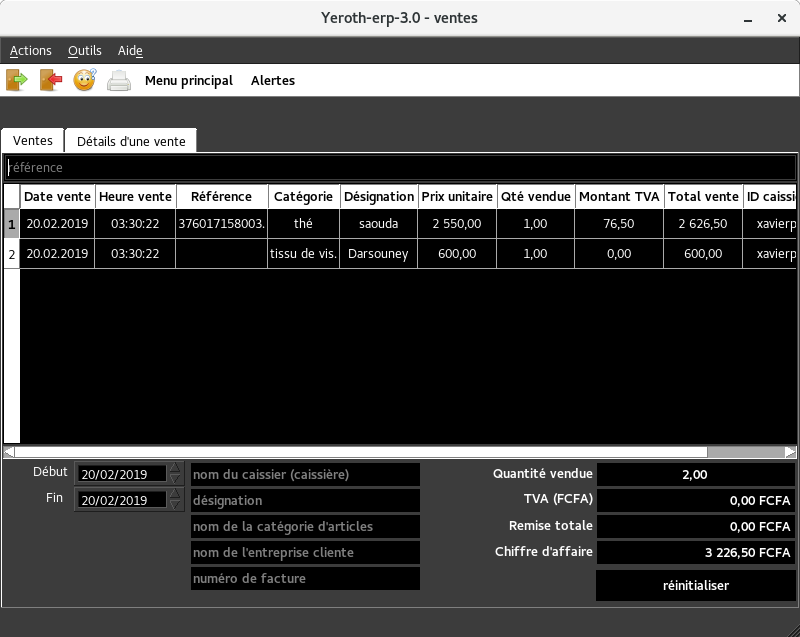
\includegraphics[scale=0.63]{images/yeren-caisse.png}
	\caption{La fen\^etre du module caisse
				(les \'etats de ventes)}~\label{fig:yeren-caisse}
\end{figure}

Le module '\textbf{Caisse}' de \yeroth donne une
vue d'ensemble sur toutes les ventes effectu\'ees.
La figure~\ref{fig:yeren-caisse} illustre
l'interface graphique du module '\textbf{Caisse}'.

%-----------------------------------------------------------

\nxsection{Voir le journal des ventes sur une p\'eriode de temps}
\index{consulter le journal des ventes}
\index{voir le journal des ventes}
\index{historique des ventes}

Un utilisateur \textbf{avec le \role \manager} d\'efinit
les dates de d\'ebut et de fin de la p\'eriode sur
laquelle il souhaite voir les ventes. Il peut aussi
ajouter les param\`etres suivants \`a sa requ\^ete:

\begin{enumerate}[1)]
	\item le nom d'un caissier 
		(champs de texte '\textbf{Caissier}')
	\item la d\'esignation d'un l'article
		(champs de texte '\textbf{D\'esignation}')
	\item une cat\'egorie d'articles
		(champs de texte '\textbf{Cat\'egorie}')
	\item le nom d'un client
		(champs de texte '\textbf{Client}')
	\item le num\'ero d'une facture.
		(champs de texte '\textbf{Facture N.}').
\end{enumerate}

Lorsque plus d'un param\`etre est utilis\'e pour la requ\^ete,
\yeroth emploi l'op\'erateur logique '\textbf{AND}' pour
g\'en\'erer la requ\^ete.

\textbf{NB:} les utilisateurs \textbf{avec le \role \caissier}
ont seulement acc\`es \`a leur journal des ventes du jour.
Ils ont aussi acc\`es au param\'etrage des \'el\'ements
suivants:

\begin{enumerate}[1)]
	\item la d\'esignation d'un l'article
		(champs de texte '\textbf{D\'esignation}')
	\item une cat\'egorie d'articles
		(champs de texte '\textbf{Cat\'egorie}')
	\item le num\'ero d'une facture.
		(champs de texte '\textbf{Facture N.}').
\end{enumerate}

%-----------------------------------------------------------

\nxsection{Voir les d\'etails d'une vente}
\index{consulter les d\'etails d'une vente}
\index{voir les d\'etails d'une vente}

Il suffit de cliquer deux fois sur la vente s\'electionn\'ee.

%-----------------------------------------------------------

\nxsection{Voir le journal des ventes d'un caissier}
\index{voir le journal des ventes d'un caissier}
\index{voir le chiffre d'affaire r\'ealis\'e avec un caissier}
\index{chiffre d'affaire d'un caissier}

Il suffit de param\'etrer la requ\^ete avec le nom de ce
caissier dans le champs de texte '\textbf{Caissier}' (Voir
la figure~\ref{fig:yeren-caisse}).

%-----------------------------------------------------------

\nxsection{Voir le journal des ventes d'un article}
\index{voir le journal des ventes d'un article}
\index{voir le chiffre d'affaire r\'ealis\'e avec un article}
\index{chiffre d'affaire d'un article}

Il suffit de param\'etrer la requ\^ete avec la d\'esignation
de cet article. Ceci se fait dans le champs de texte
'\textbf{D\'esignation}' (Voir la figure~\ref{fig:yeren-caisse}).

%-----------------------------------------------------------

\nxsection{Voir le journal des ventes d'une cat\'egorie d'articles}
\index{voir le journal des ventes d'une cat\'egorie d'articles}
\index{voir le journal des ventes d'une famille d'articles}
\index{voir le chiffre d'affaire r\'ealis\'e avec une famille d'articles}
\index{chiffre d'affaire d'une cat\'egorie d'articles}

Il suffit de param\'etrer la requ\^ete avec le nom de la
cat\'egorie de cet article. Ceci se fait dans le champs
de texte '\textbf{Cat\'egorie}' (Voir la figure~\ref{fig:yeren-caisse}).

%-----------------------------------------------------------

\nxsection{Voir le journal des achats d'un client nomm\'e}
\index{voir le journal des achats d'un client nomm\'e}
\index{voir le chiffre d'affaire r\'ealis\'e avec un client nomm\'e}

Il suffit de param\'etrer la requ\^ete avec le nom du
client concern\'e. Ceci se fait dans le champs de
texte '\textbf{Client}' (Voir la figure~\ref{fig:yeren-caisse}).

%-----------------------------------------------------------

\nxsection{Voir le journal des ventes d'une facture}
\index{voir les ventes d'une facture}

Il suffit de param\'etrer la requ\^ete avec le num\'ero
de facture correspondant. Ceci se fait dans le champs de
texte '\textbf{Facture N.}' (Voir la figure~\ref{fig:yeren-caisse}).

%-----------------------------------------------------------

\nxsection{Imprimer le journal des ventes au format PDF}
\index{Imprimer le journal des ventes au format PDF}

Il existe deux m\'ethodes pour imprimer 'le journal
des ventes' de la liste des ventes qui appara\^it \`a
la fen\^etre titr\'e '\textbf{Yeroth-erp-3.0 - Caisse}'.

\begin{itemize}[\mycheckmark{purplish}]
	\item \textcolor{purplish}{$\mathbf{1^{\text{\`ere}}}$ \textbf{m\'ethode}}\\
		Cliquer sur le lien '\textbf{Imprimer le journal des
		ventes}' qui se trouve dans le menu
		d\'eroulant '\textbf{Outils}'\\

	\item \textcolor{purplish}{$\mathbf{2^{\text{\`eme}}}$ \textbf{m\'ethode}}\\
		Presser simultan\'ement les boutons \bouton{CTRL}
		et \bouton{P} de votre clavier.
\end{itemize}

\chapter{Les Mouvements de Stocks}\label{chap:mouvements-de-stocks}

\utilisateurs: \lienmagasinier, \lienmanager.\\

\chapintro{Ce chapitre explique la diff\'erence entre une sortie
et un transfert de stocks. Il d\'ecrit aussi comment
consulter les transferts et les sorties des stocks
effectu\'es.}

\nxsection{Introduction}

\begin{figure}[!htbp]
	\centering
	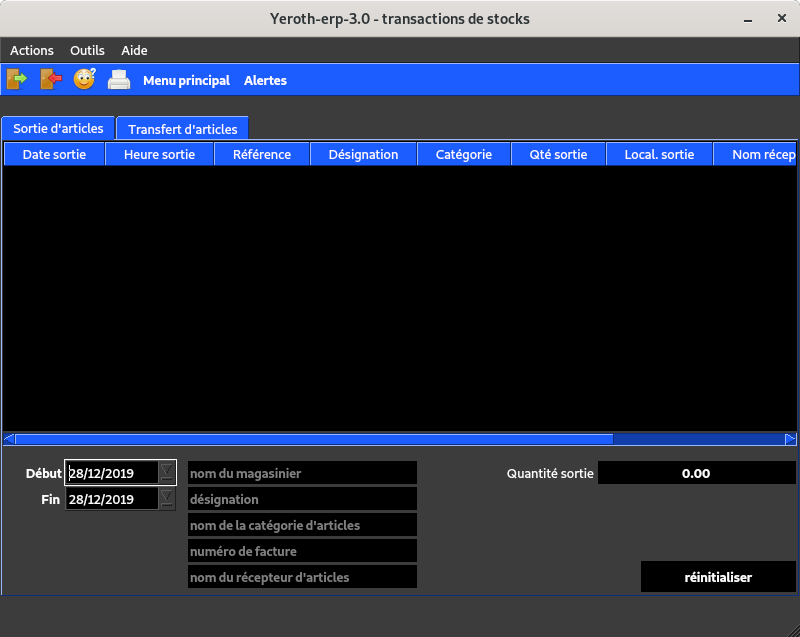
\includegraphics[scale=0.45]{images/yeren-transactions.png}
	\caption{La fen\^etre pour visualiser les sorties et les
		transferts d'articles.}
	\label{fig:yeren-transactions}
\end{figure}

La figure~\ref{fig:yeren-transactions} illustre
l'interface de \yeroth pour visualiser les sorties et les
transferts d'articles.

Dans \yeroth, une transaction est:
\begin{enumerate}[1)]
	\item une \textbf{sortie de stocks},
	\item ou bien un \textbf{transfert de stocks}.\\
\end{enumerate}

Une \textbf{sortie de stocks} est le retrait d'articles
par un client aupr\`es d'une boutique ou d'un d\'ep\^ot
de l'entreprise qui utilise \yeroth.

Un \textbf{transfert de stocks} est un mouvement de stocks
d'une boutique ou d'un d\'ep\^ot de l'entreprise vers une
boutique ou d\'ep\^ot de votre entreprise.

%--------------------------------------------------------------

\nxsection{Voir les transactions sur une p\'eriode de temps}
\index{voir les transactions sur une p\'eriode de temps}

\begin{enumerate}[1)]
	\item S\'electionnez les dates de d\'ebut et de
	fin respectivement dans les champs de dates
	'D\'ebut' et 'Fin'.
\end{enumerate}

Les transferts de stocks s'affichent automatiquement
dans le $1^{\text{er}}$ premier onglet, pendant que
les sorties de stocks s'affichent automatiquement
dans le $2^{\text{\`eme}}$ onglet.	

L'utilisateur peut aussi ajouter les param\`etres suivants
\`a sa requ\^ete :

\begin{enumerate}[1)]
	\item le nom d'un magasinier (champs de texte 
	'\textbf{Magasinier}')
	\item la d\'esignation d'un l'article 
		(champs de texte '\textbf{D\'esignation}')
	\item la cat\'egorie d'un l'article 
		(champs de texte '\textbf{Cat\'egorie}')
	\item le num\'ero d'un bon de sortie 
		(champs de texte '\textbf{Num\'ero du bon de sortie}')
	\item le nom d'un r\'ecepteur
		(champs de texte '\textbf{Nom du r\'ecepteur}').
\end{enumerate}

Lorsque plus d'un param\`etre est utilis\'e pour
la requ\^ete, \yeroth emploi l'op\'erateur logique
'\textbf{AND}' entre les diff\'erents param\`tres
pour g\'en\'erer le r\'esultat de la requ\^ete.

%--------------------------------------------------------------

\nxsection{Voir les transactions d'un magasinier}
\index{voir les transactions d'un magasinier}

\begin{enumerate}[1)]
	\item S\'electionnez dans le champs de texte
	'\textbf{Magasinier}' le nom du magasinier dont
	vous souhaitez observer les transactions effectu\'ees .
	
	\item Les transactions du magasinier choisi
	s'affichent automatiquement.
\end{enumerate}

%--------------------------------------------------------------

\nxsection{Voir les transactions d'un article}
\index{voir les transactions d'un article}

\begin{enumerate}[1)]
	\item S\'electionnez dans le champs de texte
	'\textbf{D\'esignation}' la d\'esignation de
	l'article dont vous souhaitez visualiser les
	transactions effectu\'ees .
	
	\item Les transactions de l'article choisi
	s'affichent	automatiquement.
\end{enumerate}

%--------------------------------------------------------------

\nxsection{Voir les transactions d'une cat\'egorie d'articles}
\index{voir les transactions d'une cat\'egorie d'articles}

\begin{enumerate}[1)]
	\item S\'electionnez dans le champs de texte
	'\textbf{Cat\'egorie}' le nom de la cat\'egorie
	d'articles dont	vous souhaitez visualiser
	les transactions effectu\'ees. 
	
	\item Les transactions de la cat\'egorie
	d'articles choisie s'affichent automatiquement.
\end{enumerate}

%--------------------------------------------------------------

\nxsection{Voir les transactions d'un bon de sortie}
\index{voir les transactions d'un bon de sortie}

\begin{enumerate}[1)]
	\item S\'electionnez dans le champs de texte
	'\textbf{Num\'ero du bon de sortie}' le num\'ero
	du bon de sortie dont vous souhaitez visualiser
	les transactions effectu\'ees.
	
	\item Les transactions du bon de sortie choisi
	 s'affichent automatiquement.
\end{enumerate}

%--------------------------------------------------------------

\nxsection{Voir les transactions d'un r\'ecepteur d'articles}
\index{voir les transactions d'un r\'ecepteur d'articles}

\begin{enumerate}[1)]
	\item S\'electionnez dans le champs de texte
	'\textbf{Nom du r\'ecepteur}' le nom de la
	personne dont vous souhaitez visualiser
	les transactions effectu\'ees, dont il a \'et\'e
	le r\'ecepteur.
	
	\item Les transactions de la personne choisi
	s'affichent automatiquement.
\end{enumerate}

%--------------------------------------------------------------

\nxsection{Imprimer le journal des transactions au format PDF}
\index{imprimer le journal des transactions au format PDF}

Il existe deux m\'ethodes pour imprimer 'le journal des
transactions' qui appara\^it dans la fen\^etre titr\'ee
'\textbf{Yeroth-erp-3.0 - transactions}'.

\begin{itemize}[\mycheckmark{purplish}]
	\item \textcolor{purplish}{$\mathbf{1^{\text{\`ere}}}$ \textbf{m\'ethode}}\\
		Cliquez sur le lien
		'\textbf{Imprimer le journal des sorties/transferts}'
		qui se trouve dans le menu d\'eroulant '\textbf{Outils}'.\\

	\item \textcolor{purplish}{$\mathbf{2^{\text{\`eme}}}$ \textbf{m\'ethode}}\\
		Pressez simultan\'ement les boutons \bouton{CTRL}
		et \bouton{P} de votre clavier.
\end{itemize}

Un fichier au format PDF est alors g\'en\'er\'e et affich\'e.

\begin{figure}[!htbp]
	\centering
	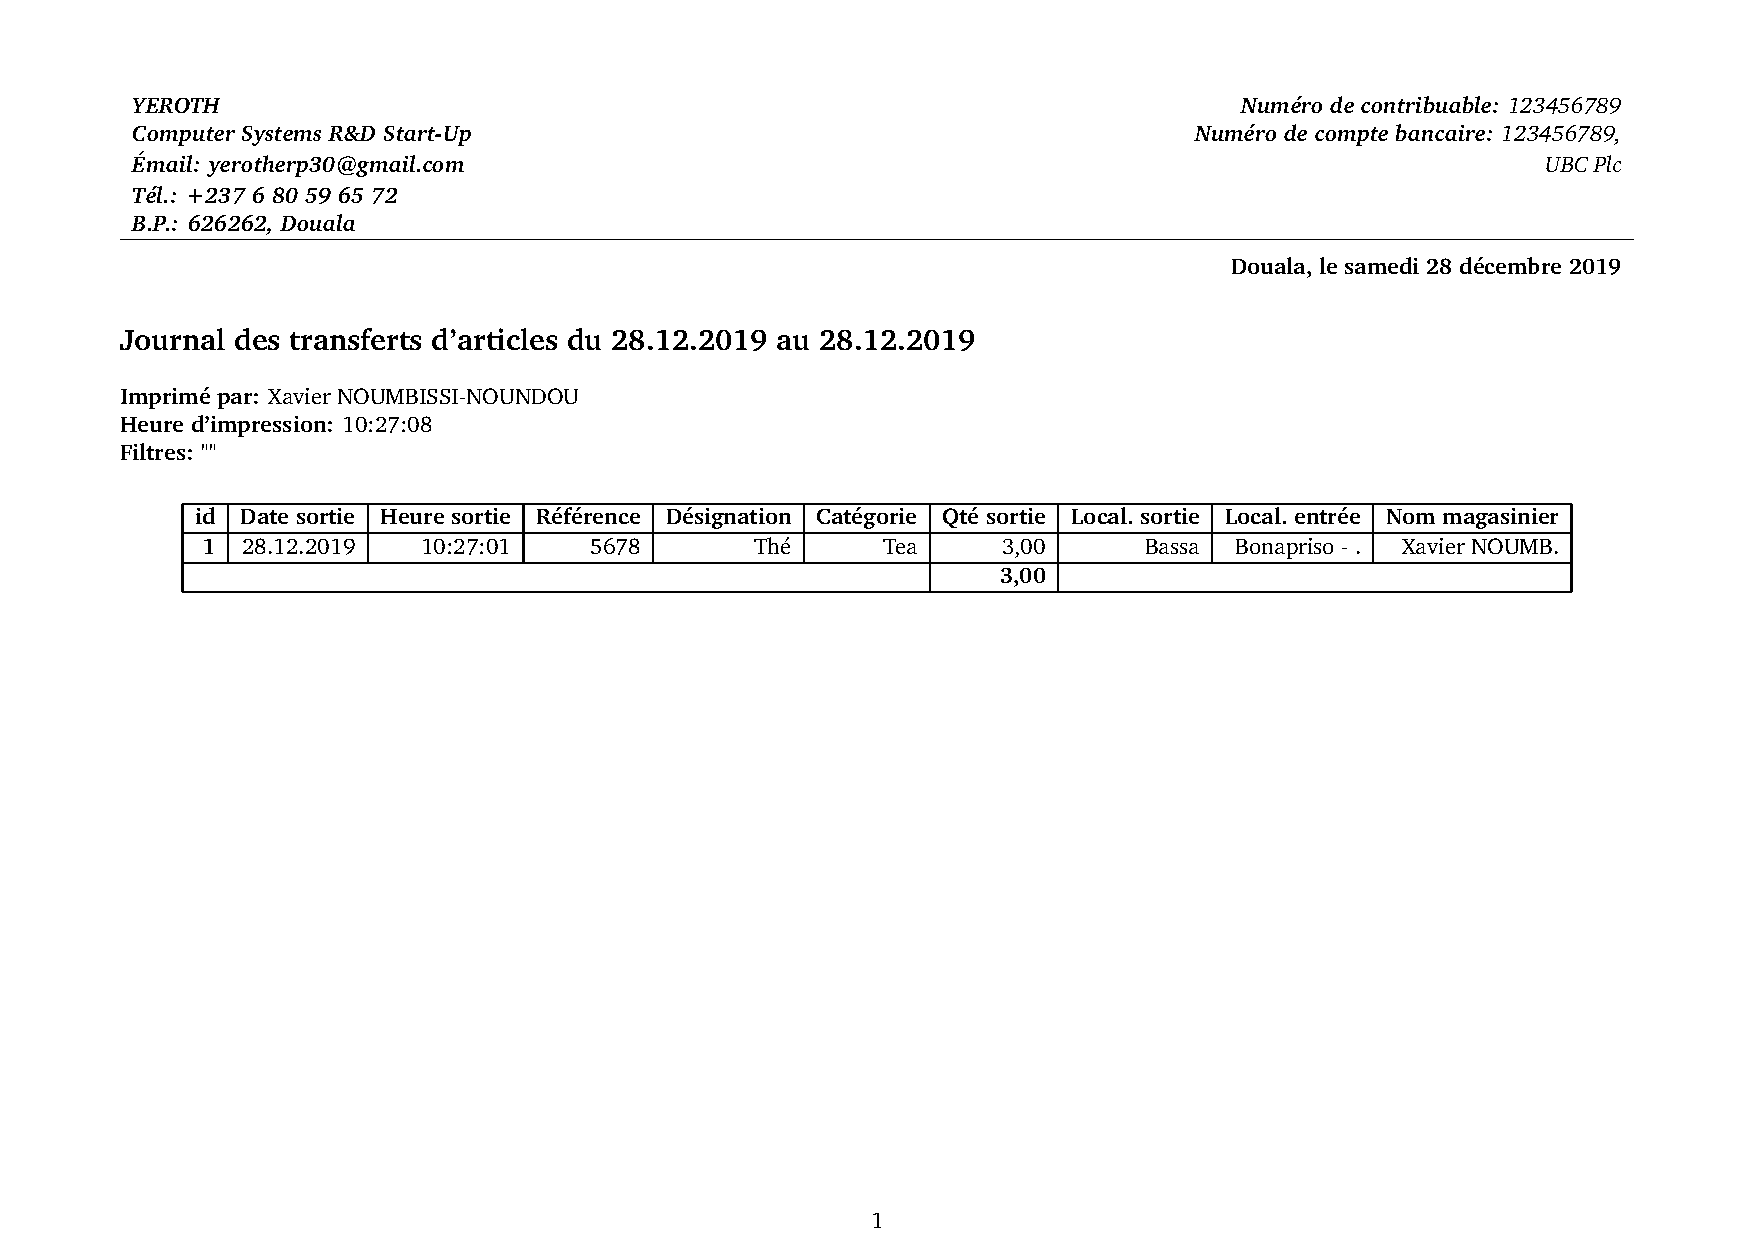
\includegraphics[scale=0.55]{images/yeren-journal-sortie-stocks-2017-06-14.pdf}
	\caption{Un journal de sorties des stocks.}
	\label{fig:yeren-journal-sorties-des-stocks}
\end{figure}

La figure~\ref{fig:yeren-journal-sorties-des-stocks} illustre un
exemple de journal de sorties des stocks au format PDF.

%--------------------------------------------------------------

\chapter{Les Tableaux de Bords}\label{chap:tableaux-de-bords}
\index{les tableaux de bords}

\utilisateurs: \lienmanager.\\

\chapintro{Ce chapitre d\'ecrit comment consulter les
		 	tableaux de bord. En effet, bon nombre de
		 	d\'ecisions des \manager proviennent de la
		 	visualisation des rapports financiers, et
		 	commerciaux.}

\nxsection{Introduction}\label{sec:tableaux-introduction}

\begin{figure}[!htbp]
	\centering
	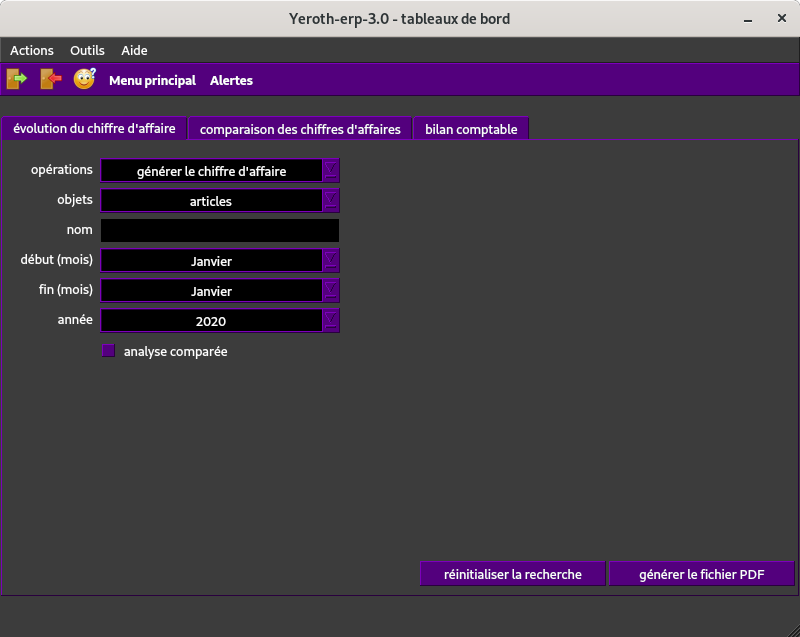
\includegraphics[scale=0.45]{images/yeren-rapports.png}
	\caption{La fen\^etre principale pour g\'en\'erer les tableaux de bords.}
	\label{fig:yeroth-tableaux}
\end{figure}

La figure~\ref{fig:yeren-rapports} illustre l'interface
de \yeren pour param\'etrer et g\'en\'erer l'\'evolution
du chiffre d'affaire (au format PDF) sur une p\'eriode de temps.

L'interface graphique 'comparaison des chiffres d'affaires'
(figure~\ref{fig:yeren-rapports-comparaison-articles})
permet \`a l'utilisateur de comparer les chiffres
d'affaire d'objets allant de $2$ \`a $9$ unit\'es.

Les objets de comparaisons sont les suivants:
\begin{enumerate}[1)]
	\item le chiffre d'affaire des articles vendus
	\item le chiffre d'affaire des cat\'egories d'articles vendues
	\item le chiffre d'affaire des clients nomm\'es de l'entreprise
	\item le chiffre d'affaire des caissiers de l'entreprise.\\
\end{enumerate}

L'utilisateur a le choix entre les diagrammes comparatifs
suivants:
\begin{enumerate}[1)]
	\item le diagramme en bande
	\item le diagramme circulaire.\\
\end{enumerate}

La figure~\ref{fig:diagramme-bande-chiffre-daffaire-comparatif-articles}
et~\ref{fig:diagramme-circulaire-chiffre-daffaire-comparatif-articles}
illustrent des examples de diagramme comparatif en 'diagramme en bande'
et en 'diagramme circulaire' respectivement.

\nxsection{G\'en\'erer l'\'evolution du chiffre
			d'affaire}\label{sec:evolution-chiffre-affaire}
\index{g\'en\'erer l'\'evolution du chiffre d'affaire}
\index{\'evolution du chiffre d'affaire}

Il faut effectuer les actions suivantes dans l'interface
graphique de \yeren illustr\'ee dans la
figure~\ref{fig:yeren-rapports}:

\begin{enumerate}[1)]
	\item choisir la date de 'd\'ebut (mois)'
	\item choisir la date de 'fin (mois)'	
	\item choisir l'ann\'ee souhait\'ee
	\item conclure an cliquant dur le
		bouton \bouton{g\'en\'erer le fichier PDF}.
\end{enumerate}

%-----------------------------------------------------------
\newpage
\nxsection{G\'en\'erer les chiffres d'affaires de plusieurs
	articles de fa\c{c}on comparative
	}\label{sec:comparaison-chiffre-affaire-articles}
\index{g\'en\'erer les chiffres d'affaires de plusieurs	articles de fa\c{c}on comparative}
\index{comparer les chiffres d'affaires de plusieurs articles}

La figure~\ref{fig:yeren-rapports-comparaison-articles}
illustre comment g\'en\'erer un diagramme en bande,
comparatif des quatre articles avec les chiffres d'affaires
les plus \'elev\'es.\\

\begin{figure}[!htbp]
	\centering
	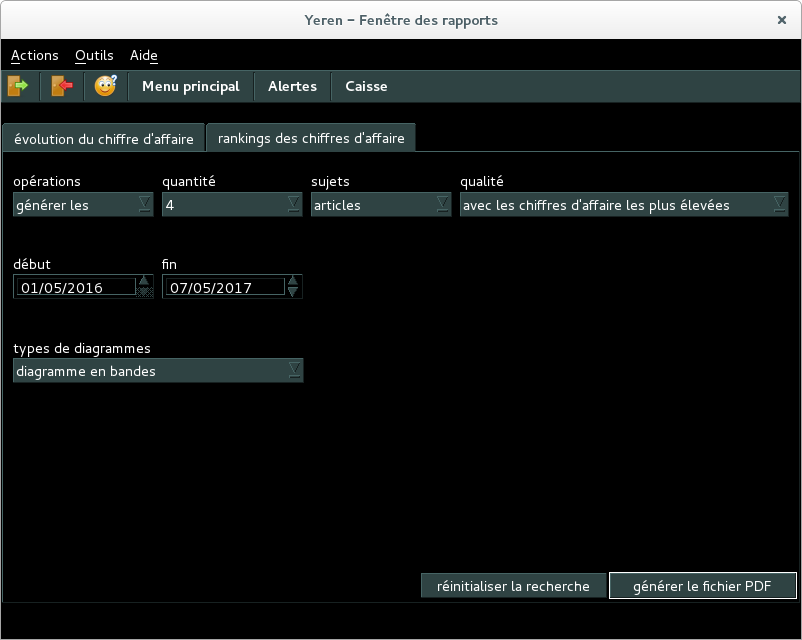
\includegraphics[scale=0.45]{images/yeren-rapports-comparaison-articles.png}
	\caption{Une figure comparative des chiffres d'affaires de
		quatre articles de la fen\^etre des rapports commerciaux.}
	\label{fig:yeroth-tableaux-comparaison-articles}
\end{figure}

La figure~\ref{fig:diagramme-bande-chiffre-daffaire-comparatif-articles}
illustre le fichier PDF g\'en\'er\'e avec pour option 'diagramme en bandes'.

%\newpage

\begin{figure}[!htbp]
	\centering
	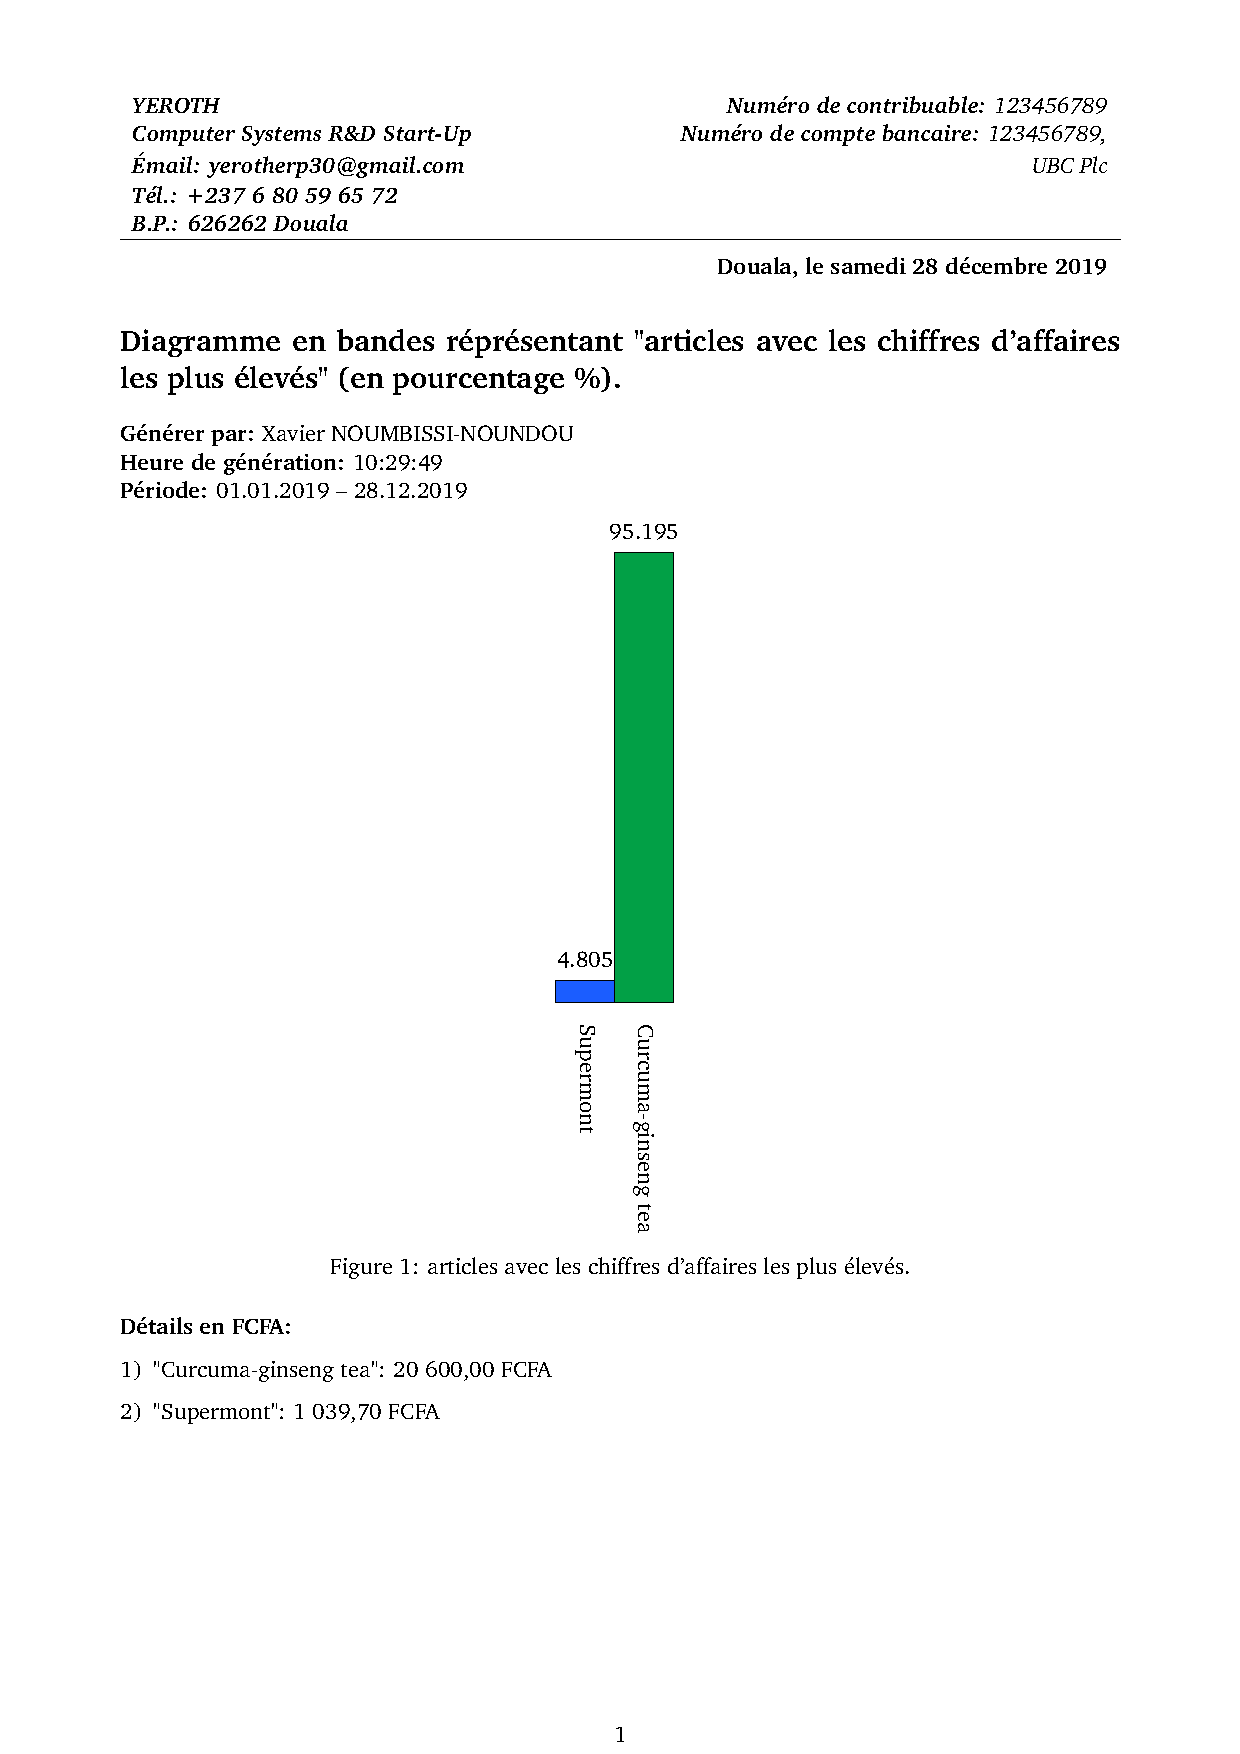
\includegraphics[scale=0.65]{images/diagramme-bande-chiffre-daffaire-comparatif-articles.pdf}
	\caption{Une figure comparative du chiffre d'affaire de
		plusieurs articles \`a l'aide d'un digramme en bande.}
	\label{fig:diagramme-bande-chiffre-daffaire-comparatif-articles}
\end{figure}

La figure~\ref{fig:diagramme-circulaire-chiffre-daffaire-comparatif-articles}
illustre le fichier PDF g\'en\'er\'e avec pour option 'diagramme circulaire'.

\begin{figure}[!htbp]
	\centering
	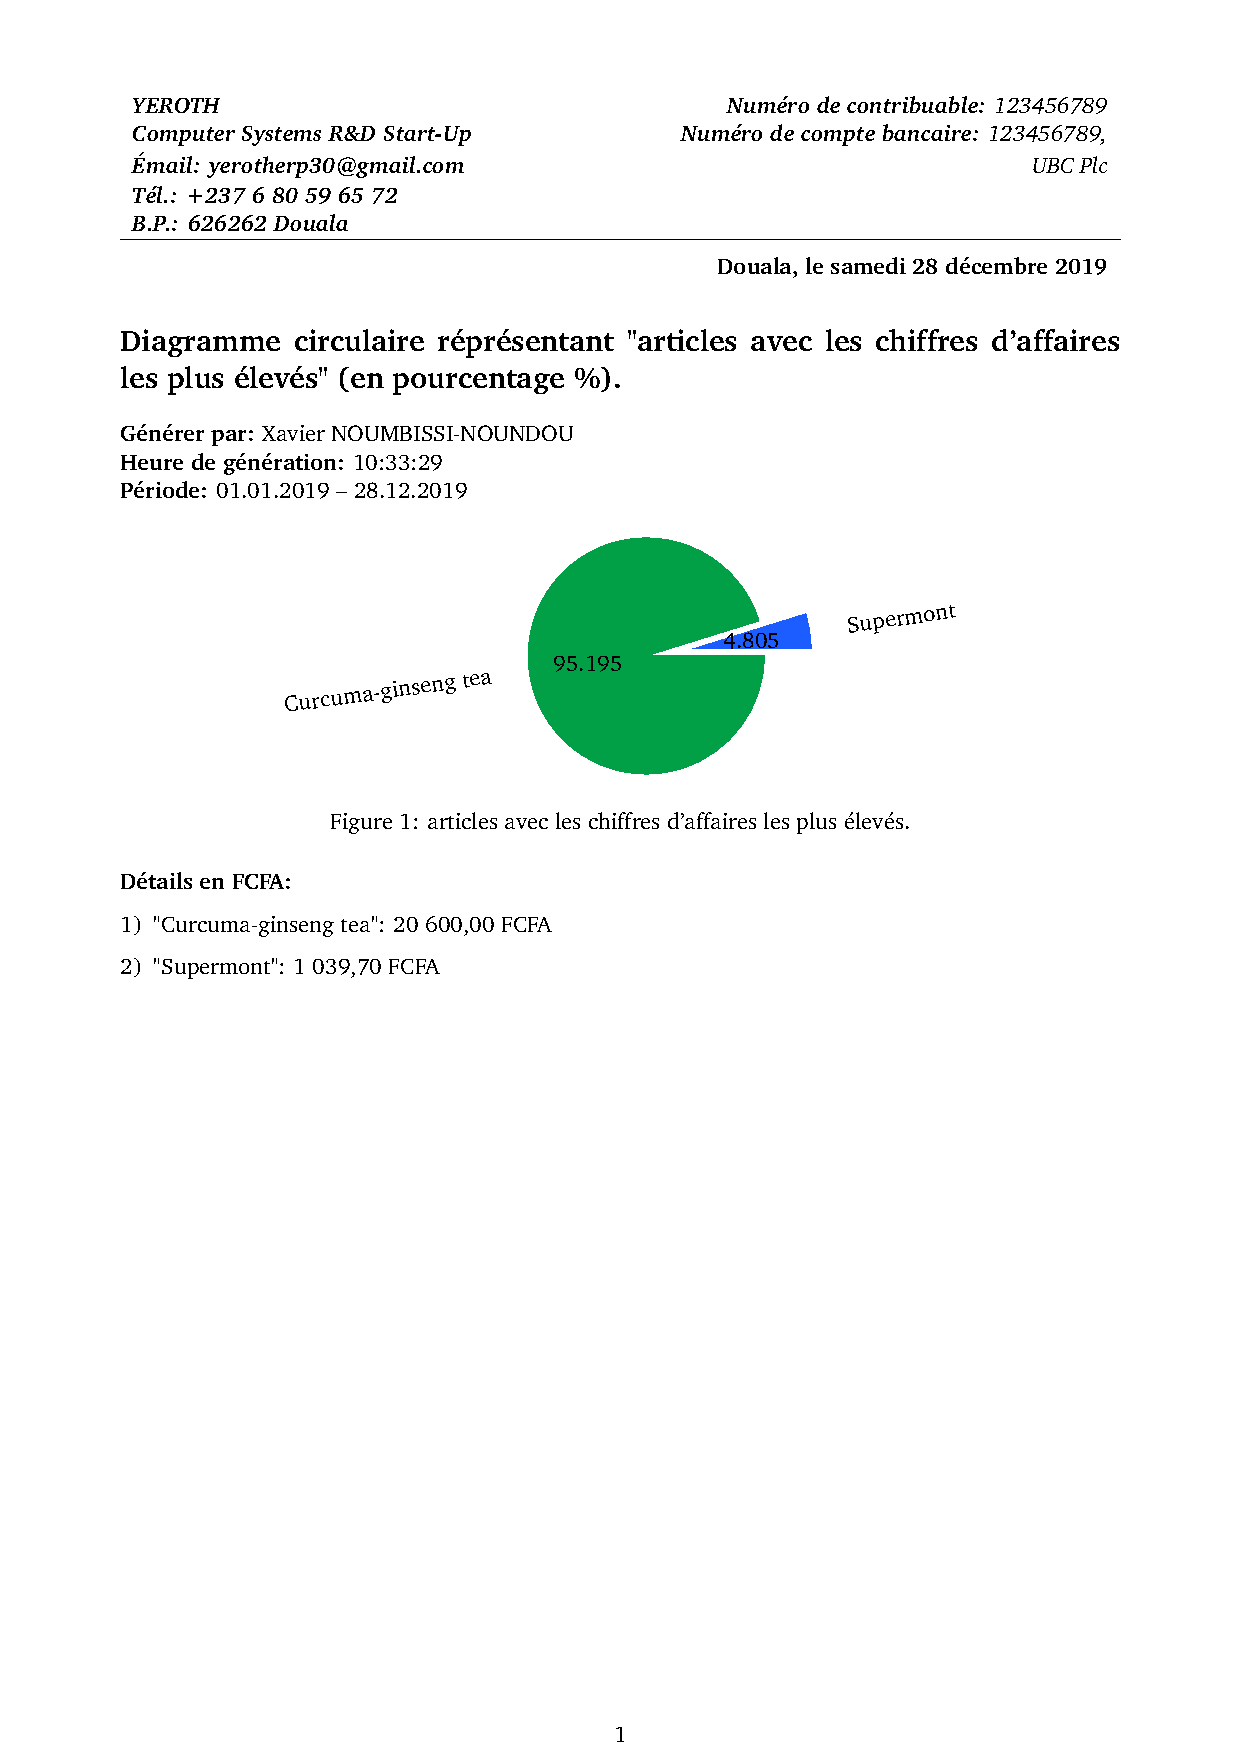
\includegraphics[scale=0.65]{images/diagramme-circulaire-chiffre-daffaire-comparatif-articles.pdf}
	\caption{Une figure comparative du chiffre d'affaires de
		plusieurs articles \`a l'aide d'un digramme circulaire.}
	\label{fig:diagramme-circulaire-chiffre-daffaire-comparatif-articles}
\end{figure}

%-----------------------------------------------------------

\newpage
\nxsection{G\'en\'erer les chiffres d'affaires de plusieurs
			cat\'egories articles de fa\c{c}on comparative}
\index{g\'en\'erer les chiffres d'affaires de plusieurs
		cat\'egories articles de fa\c{c}on comparative}

Il faut proc\'eder comme \`a la section~\ref{sec:comparaison-chiffre-affaire-articles}, juste
en changeant le combo box '\textbf{sujets}' d'articles \`a
'\textbf{cat\'egories}' et le combo box '\textbf{qualit\'e}'.

%-----------------------------------------------------------

\nxsection{G\'en\'erer les chiffres d'affaires de plusieurs
			clients de fa\c{c}on comparative}
\index{g\'en\'erer les chiffres d'affaires de plusieurs 
		clients de fa\c{c}on comparative}

Il faut proc\'eder comme \`a la section~\ref{sec:comparaison-chiffre-affaire-articles}, juste
en changeant le combo box '\textbf{sujets}' d'articles \`a
'\textbf{clients}' et le combo box '\textbf{qualit\'e}'.

%-----------------------------------------------------------

\nxsection{G\'en\'erer les chiffres d'affaires de plusieurs
			caissiers de fa\c{c}on comparative}
\index{g\'en\'erer les chiffres d'affaires de plusieurs
		caissiers de fa\c{c}on comparative}

Il faut proc\'eder comme \`a la section~\ref{sec:comparaison-chiffre-affaire-articles}, juste
en changeant le combo box '\textbf{sujets}' d'articles \`a
'\textbf{caissiers}' et le combo box '\textbf{qualit\'e}'.


\chapter{Les Informations G\'en\'erales}\label{chap:informations-generales}

\utilisateurs: \lienadmin, \liencaissier, \lienmagasinier, \lienmanager.\\

\chapintro{Ce chapitre d\'ecrit comment avoir acc\`es aux
informations publiques de l'entreprise et de \yeroth
(ex.: le si\`ege social de l'entreprise, la version
de \yeroth utilis\'ee, etc).}

\nxsection{Voir les d\'etails de l'utilisateur avec lequel
			on s'est enregistr\'e}
\index{voir les d\'etails de l'utilisateur avec lequel
		on s'est enregistr\'e}

\begin{figure}[!htbp]
	\centering
	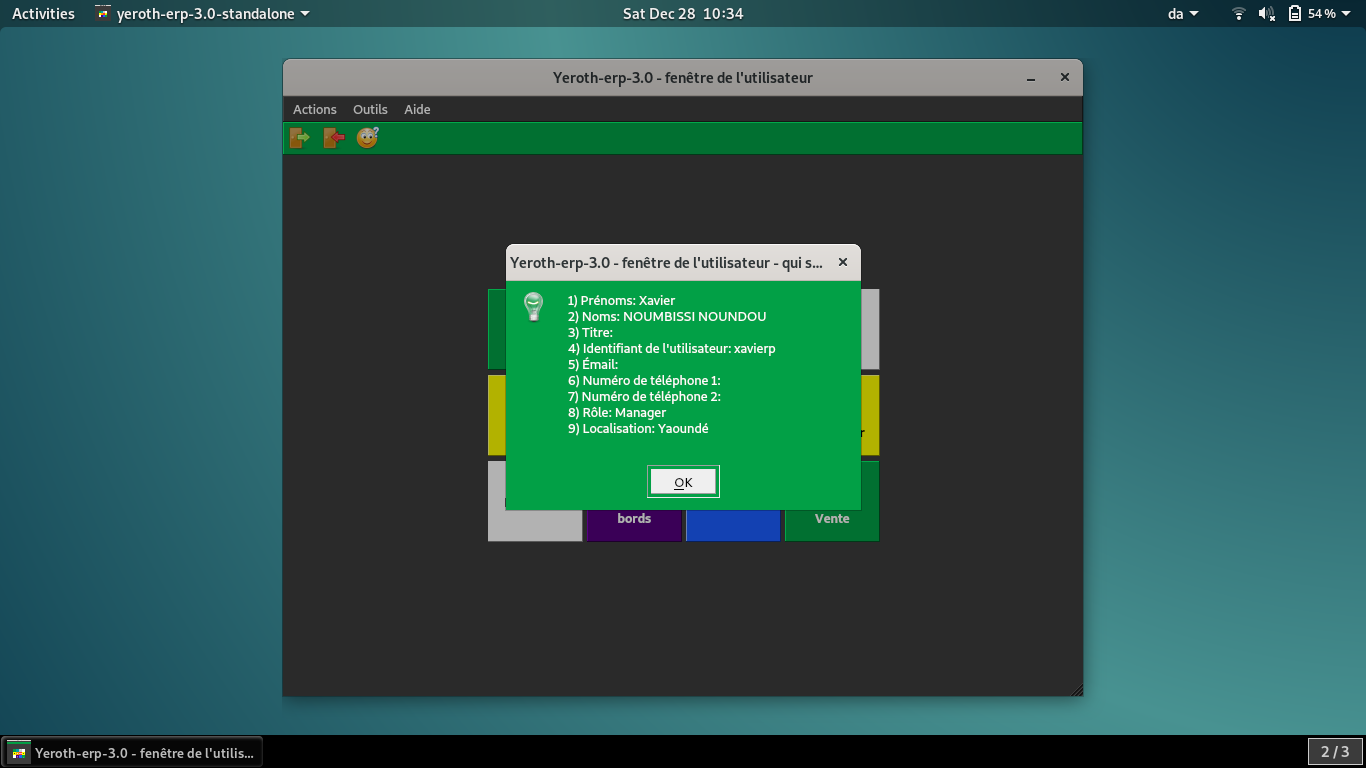
\includegraphics[scale=0.34]{images/yeren-qui-suis-je.png}
	\caption{Un example de la fonctionalit\'e 'Qui suis je ?'.}
	\label{fig:yeren-qui-suis-je}
\end{figure}

La figure~\ref{fig:yeren-qui-suis-je} illustre un example de
la fonctionalit\'e '\textbf{Qui suis je ?}'.

\`A partir de n'importe quelle fen\^etre de \yeroth, cliquez
sur le lien '\textbf{Qui suis je ?}' dans le menu d\'eroulant
'\textbf{Outils}' pour obtenir les informations suivantes
de l'utilisateur avec lequel on s'est enregistr\'e:

\begin{enumerate}[1)]
	\item l'\'email
	\item l'identification de l'utilisateur	
	\item la localisation
	\item les noms	
	\item le num\'ero de t\'el\'ephone 1
	\item le num\'ero de t\'el\'ephone 2	
	\item les pr\'enoms
	\item le r\^ole	
	\item le titre.
\end{enumerate}

%---------------------------------------------------------------

\nxsection{Voir les informations g\'en\'erales de l'entreprise}
\index{voir les informations g\'en\'erales de l'entreprise}

\`A partir de n'importe quelle fen\^etre de \yeroth (except\'e
les fen\^etres de l'administration), cliquez
sur le lien '\textbf{Informations sur l'entreprise}' dans
le menu d\'eroulant '\textbf{Aide}' pour obtenir les
informations suivantes de l'entreprise o\`u \yeroth
est ainsi d\'eploy\'e:

\begin{enumerate}[1)]
	\item l'\'email
	\item l'adresse
	\item la bo\^ite postale
	\item la d\'enomination de l'entreprise
	\item la localisation
	\item le num\'ero de contribuable	
	\item le pays
	\item les secteurs d'activit\'es
	\item le si\`ege social
	\item le t\'el\'ephone
	\item la ville.
\end{enumerate}

La figure~\ref{fig:yeren-informations-generales-entreprise}
illustre un example de la fonctionalit\'e 
'\textbf{Informations sur l'entreprise}'.\\

\begin{figure}[!htbp]
	\centering
	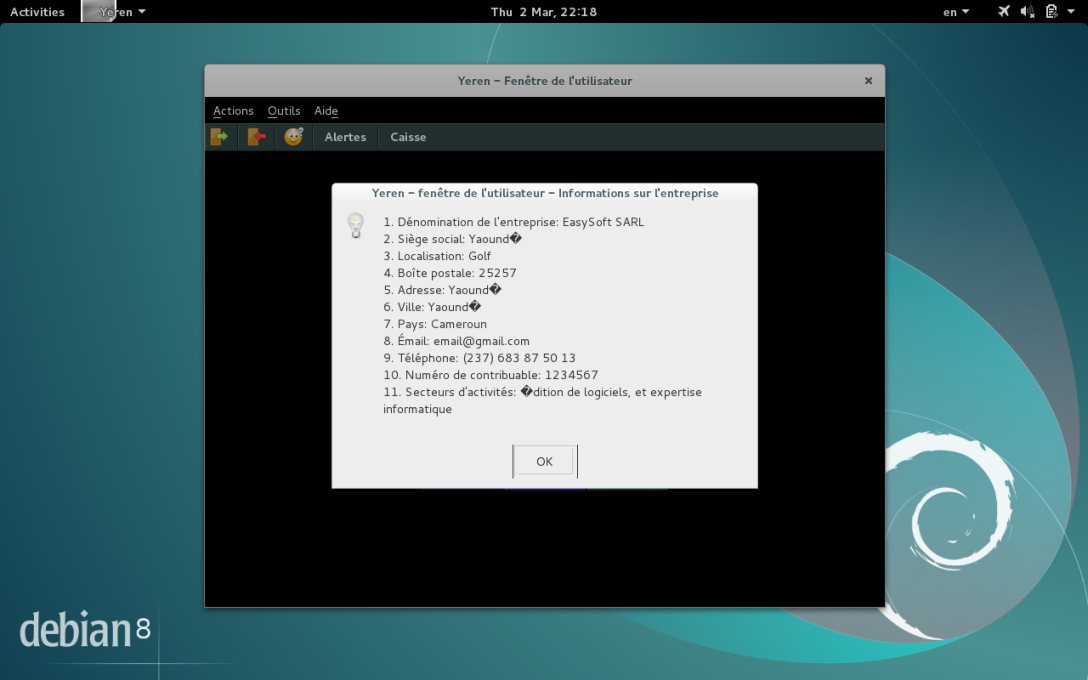
\includegraphics[scale=0.4]{images/yeren-informations-generales-entreprise.png}
	\caption{Un example de la fonctionalit\'e 'Informations sur l'entreprise'.}
	\label{fig:yeren-informations-generales-entreprise}
\end{figure}

%---------------------------------------------------------------

\newpage
\nxsection{Voir le manuel de l'utilisateur au format PDF}
\index{manuel de l'utilisateur au format PDF}

Il suffit de cliquer sur le lien '\textbf{Manuel de l'utilisateur (PDF)}'
qui se trouve dans le menu '\textbf{Aide}' de la fen\^etre
principale de chaque type d'utilisateur de \yeroth:

\begin{enumerate}[1)]
	\item \admin (voir figure~\ref{fig:fenetre-principale-admin})
	\item \caissier (voir figure~\ref{fig:fenetre-principale-caissier})
	\item \magasinier (voir figure~\ref{fig:yeren-fenetre-magasinier})
	\item \manager (voir figure~\ref{fig:yeren-fenetre-patron}).		
\end{enumerate}

%---------------------------------------------------------------

\nxsection{Voir la version de \yeroth que vous utilis\'e}
\index{voir la version de \yeroth que vous utilis\'e}

Il suffit de cliquer sur le lien '\textbf{\`A propos}' qui
se trouve dans le menu '\textbf{Aide}' de n'importe quelle
fen\^etre de \yeroth.

La figure~\ref{fig:yeren-apropos}
illustre un example de la fonctionalit\'e 
'\textbf{\`A propos}'.

\begin{figure}[!htbp]
	\centering
	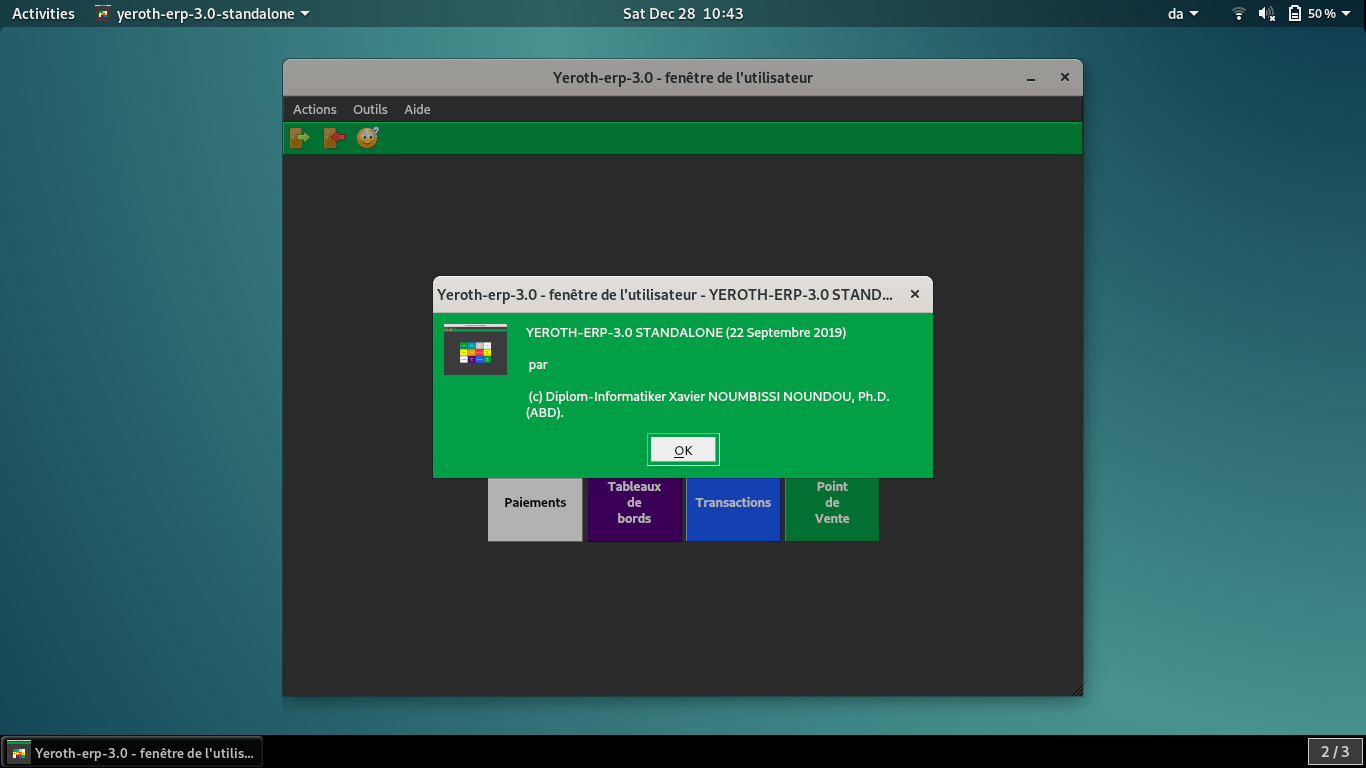
\includegraphics[scale=0.369]{images/yeren-apropos.png}
	\caption{Un example de la fonctionalit\'e '\`A propos'.}
	\label{fig:yeren-apropos}
\end{figure}



\chapter{L'Administration de \yeroth}\label{chap:administration-logiciel}

\utilisateurs: \lienadmin, \lienmanager.\\

\chapintro{Ce chapitre d\'ecrit comment effectu\'e
les t\^aches d'administration (ex: cr\'eer un
nouveau compte pour un utilisateur, etc.).}

\nxsection{Introduction}

\begin{figure}[!htpb]
\centering
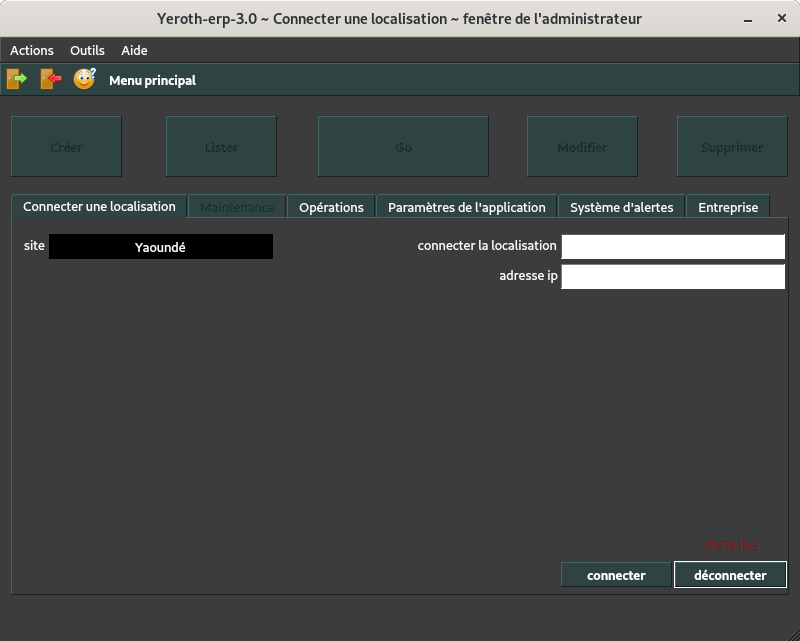
\includegraphics[scale=0.45]{images/yeroth-fenetre-administrateur.png}
\caption{La fen\^etre de l'administrateur.}
\label{fig:fenetre-administrateur}
\end{figure}

La figure~\ref{fig:fenetre-administrateur} illustre la
fen\^etre d'acceuil de l'administration de \yeroth.

On y arrive automatiquement lorsqu'on s'enregistre
\`a \yeroth avec un utilisateur du \role \admin.

Avec un utilisateur du \role \manager, on clique sur le
bouton \bouton{Administration} \`a partir de l'interface
d'acceuil des utilisateurs du \role \manager 
(voir figure~\ref{fig:yeren-fenetre-patron}).

\newpage

%%%%%%%%%%%%%%%%%%%%%%%%%%%%%%%%%%%%%%%%%%%%%%%%%%%%%%%%%%%%%%%%%%%%%%%%%%%%%%%%%

\nxsection{La connection \`a d'autres localisations}
\index{connection \`a d'autres localisations}

La figure~\ref{fig:yeren-admin-connection-autres-db}
illustre l'interface graphique de connection \`a la
base de donn\'ees d'une autre localisation;
cette interface graphique est le $1^{\text{er}}$ onglet
de la fen\^etre de l'administration.

\begin{figure}[!htpb]
	\centering
	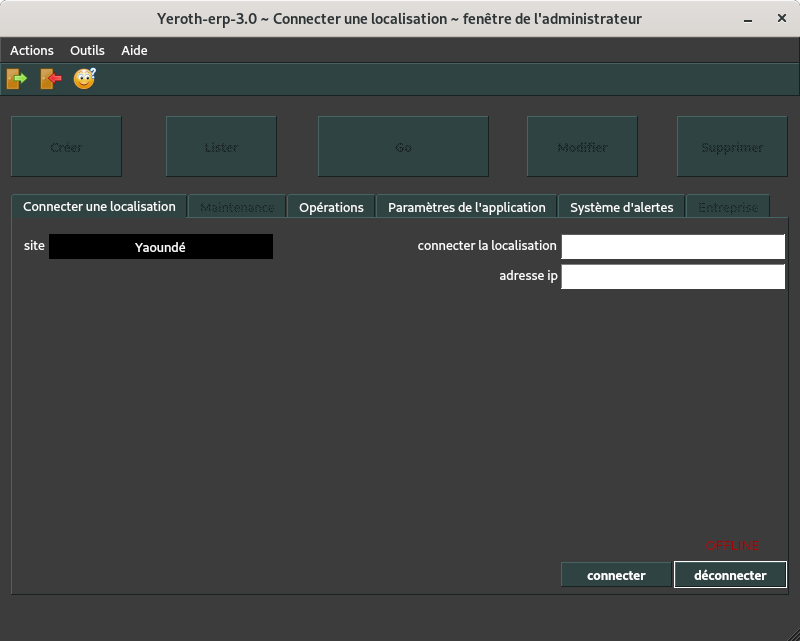
\includegraphics[scale=0.45]{images/yeren-admin-connection-autres-db.png}
	\caption{l'interface graphique de connection de
		\yeroth \`a d'autres localisations.}\label{fig:yeren-admin-connection-autres-db}
\end{figure}

Voici la proc\'edure par laquelle l'utilisateur peut
connecter son installation de \yeroth \`a la base de donn\'ees
d'autres localisations:
\begin{enumerate}[1)]
	\item choisir dans le champs de texte '\textbf{localisation}'
		le nom de localisation \`a laquelle on souhaite
		se connecter. Lorsque cela est fait, l'adresse IP
		de la localisation choisie est automatiquement
		affich\'ee dans le champs de texte '\textbf{adresse IP}'
	
	\item cliquer sur le bouton \bouton{connecter}.
\end{enumerate}

Si la connection est r\'eussie, le mot 
'\textbf{\textcolor{forestgreen}{ONLINE}}' est affich\'e en
couleur verte au dessus du bouton \bouton{connecter}.

%%%%%%%%%%%%%%%%%%%%%%%%%%%%%%%%%%%%%%%%%%%%%%%%%%%%%%%%%%%%%%%%%%%%%%%%%%%%%%%%%

\nxsection{Les param\`etres g\'en\'eraux}
\index{param\`etres g\'en\'eraux}

La figure~\ref{fig:yeren-parametres} illustre l'interface
graphique des param\`etres g\'en\'eraux de \yeroth;
cette interface graphique est le $4^{\text{\`eme}}$
onglet de la fen\^etre de l'administration de \yeroth.

\begin{figure}[!htpb]
	\centering
	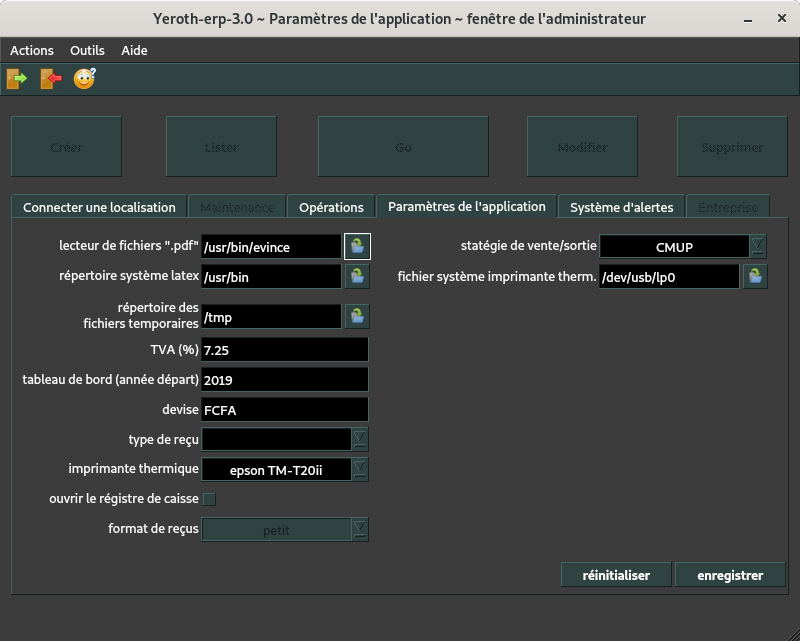
\includegraphics[scale=0.45]{images/yeroth-administration-parametres-generaux.png}
	\caption{l'interface graphique de param\'etrage g\'en\'eral
		de \yeroth.}\label{fig:yeren-parametres}
\end{figure}

Les param\`etres g\'en\'eraux qui peuvent \^etre
modifi\'es sont les suivants:
\begin{enumerate}[1)]
	\item le lecteur des fichiers PDF
	\item le compilateur des fichiers '.tex'
	\item le r\'epertoire des fichiers temporaraires
	\item la taxe sur la valeur ajout\'e
	\item la strat\'egie de vente/sortie des stocks (\cmup, \dpfdpo, \fifo, \lifo)
		\begin{enumerate}[1)]
			\item la s\'election de \cmup pr\'esente tous les
				stocks pr\'esents dans la base de donn\'ees \index{\cmup}
			\item la s\'election \dpfdpo pr\'esente tous les
				stocks selon la strat\'egie ''\textbf{Date of Preemption,
				First Date of Preemption Out}'' \index{\dpfdpo}				
			\item la s\'election de \fifo pr\'esente tous les
				stocks selon la start\'egie ''\textbf{First In, First Out}''
				\index{\fifo}
			\item la s\'election de \lifo pr\'esente tous les
				stocks selon la strat\'egie ''\textbf{Last In, First Out}''
				\index{\lifo}
		\end{enumerate}
	\item le format des fichiers de facturations
	\item l'ann\'ee de d\'epart des rapports lors de la
			g\'en\'eration des chiffres d'affaire.\\
\end{enumerate}

Les strat\'egies de gestion des stocks sont d\'ecrites
dans la section~\ref{sec:strategies-gestion-stocks}.

%%%%%%%%%%%%%%%%%%%%%%%%%%%%%%%%%%%%%%%%%%%%%%%%%%%%%%%%%%%%%%%%%%%%%%%%%%%%%%%%%

\newpage
\nxsection{Les param\`etres du syst\`eme d'alertes}
\index{param\`etres du syst\`eme d'alertes}

La figure~\ref{fig:yeren-admin-alertes-config} illustre
l'interface graphique des param\`etres du syst\`eme d'alertes
de \yeroth; cette interface graphique est le $5^{\text{\`eme}}$
onglet de la fene\^etre de l'administration de \yeroth.

\begin{figure}[!htpb]
	\centering
	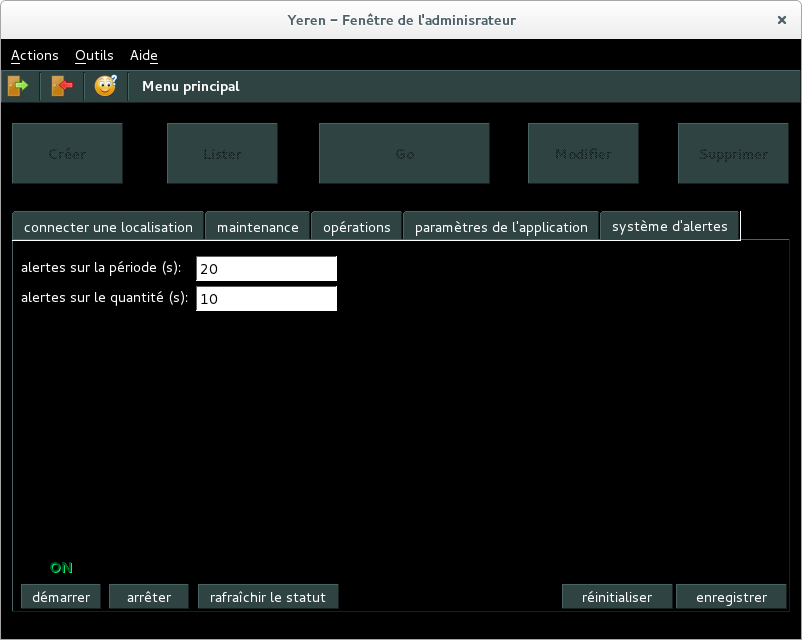
\includegraphics[scale=0.45]{images/yeren-admin-alertes-config.png}
	\caption{l'interface graphique de param\'etrage du
		syst\`eme d'alertes \yeroth.}\label{fig:yeren-admin-alertes-config}
\end{figure}

Le syst\`eme d'alertes est d\'emarr\'e par d\'efaut lors du
d\'emarrage de l'ordinateur. 

Il faut d\'emarrer l'interface graphique de \yeroth en tant
qu'administrateur du syst\`eme d'exploitation afin de
pouvoir stopper le syst\`eme d'alertes lorsqu'il a \'et\'e
d\'emarr\'e lors du d\'emarrage de l'ordinateur.

Les param\`etres du syst\`eme d'alertes qui peuvent \^etre
modifi\'es sont les suivants:
\begin{enumerate}[1)]
	\item \textbf{alertes sur la p\'eriode (s)}: d\'efinit
		l'intervalle de temps (en secondes) apr\`es lequel
		\yeroth visite la base de donn\'ees pour voir
		s'il y'a de nouvelles alertes sur les p\'eriodes de temps
		
	\item \textbf{alertes sur la quantit\'e (s)}: d\'efinit
		l'intervalle de temps (en secondes) apr\`es lequel
		\yeroth visite la base de donn\'ees pour voir
		s'il y'a de nouvelles alertes sur les quantit\'es en stocks.\\
\end{enumerate}

Cette interface graphique permet aussi:
\begin{enumerate}[1)]
	\item de \textbf{d\'emarrer le syst\`eme d'alertes} en pressant
		sur le bouton \bouton{d\'emarrer}. Lorsque le syst\`eme
		d'alertes est en marche, le mot anglais
		'\textbf{\textcolor{forestgreen}{ON}}' est
		affich\'e en vert au dessus du boutton \bouton{d\'emarrer}.
		
	\item \textbf{d'arr\^eter le syst\`eme d'alertes} en pressant
		sur le bouton \bouton{arr\^eter}. Lorsque le syst\`eme
		d'alertes n'est pas en marche, le mot anglais
		'\textbf{\textcolor{firebrickred}{OFF}}' est
		affich\'e en couleur rouge au dessus du boutton \bouton{arr\^eter}.
		
		Cette action n\'ecessite que l'utilisateur est d\'emarr\'e
		\yeroth en tant qu'administrateur du syst\`eme d'exploitation.
		
	\item \textbf{d'actualiser le statut} dans lequel se trouve
		le syst\`eme d'alertes en pressant sur le bouton
		\bouton{rafra\^ichir le statut}.		
\end{enumerate}
%-----------------------------------------------------------

\newpage
\nxsection{Les Alertes}\label{sec:administration-alertes}
\index{les alertes}

\nxsubsection{Afficher les d\'etails d'une alerte}
\index{afficher les d\'etails d'une alerte}

La figure~\ref{fig:admin-alertes-afficher-details} illustre
l'interface graphique de \yeroth qui affiche les d\'etails
d'une alerte.\\

\begin{figure}[!htpb]
	\centering
	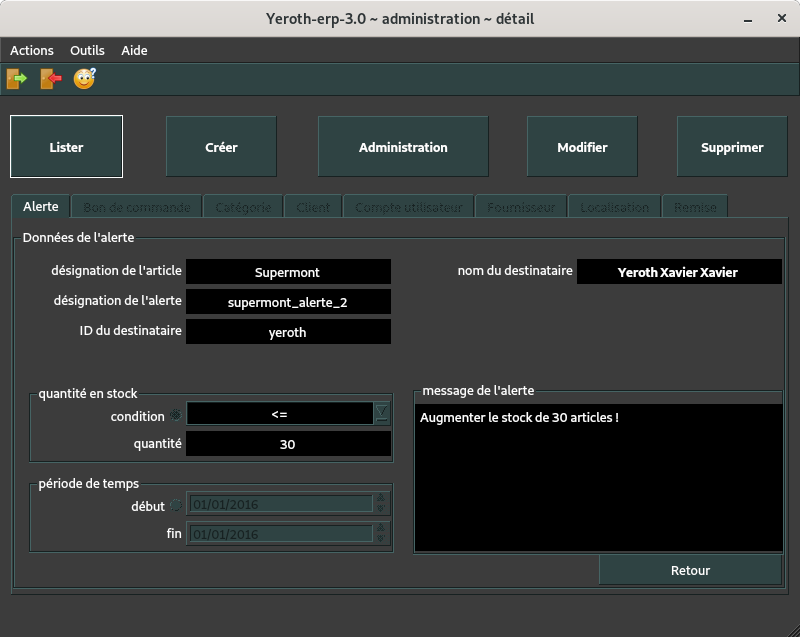
\includegraphics[scale=0.45]{images/alerte-afficher-details.png}
	\caption{Une interface graphique de \yeroth qui affiche les d\'etails
	d'une alerte.}\label{fig:admin-alertes-afficher-details}
\end{figure}

\procparagraph{Proc\'edure pour afficher les d\'etails d'une alerte}
\begin{enumerate}[1)]
	\item \`A partir de l'interface graphique de l'acceuil de
		l'administration (voir figure~\ref{fig:fenetre-administrateur}),
		on clique sur l'onglet intitul\'e \textbf{op\'erations}. 
		
	\item Choisir '\textbf{lister}' dans le '\emph{combo box
		op\'erations}'.
		
	\item Choisir '\textbf{une alerte}' dans le '\emph{combo box
		sujets}'. Vous \^etes automatiquement conduit \`a la fen\^etre
		illustr\'ee par la figure~\ref{fig:admin-alertes-lister}.
		
	\item S\'electionner l'alerte dont vous souhaitez afficher
		les d\'etails dans la liste des alertes affich\'ee.
		
	\item Cliquer sur le bouton \bouton{Afficher}. Les d\'etails
		sur le stock sont affich\'es dans une nouvelle fen\^etre.
\end{enumerate}

%%%%%%%%%%%%%%%%%%%%%%%%%%%%%%%%%%%%%%%%%%%%%%%%%%%%%%%%%%%%%%%%%%%%%%%%%%%%%%%%%

\newpage
\nxsubsection{Cr\'eer une alerte}\label{sec:administration-alertes-creer}
\index{cr\'eer une alerte}

La figure~\ref{fig:admin-alertes-creer} illustre l'interface
graphique de \yeroth pour cr\'eer une alerte.\\

\begin{figure}[!htpb]
	\centering
	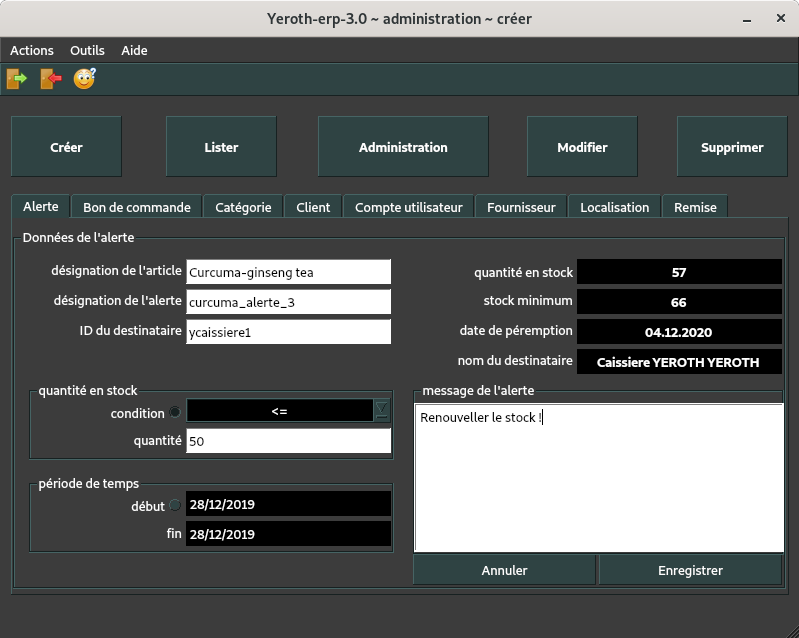
\includegraphics[scale=0.45]{images/alerte-creer.png}
	\caption{L'interface graphique pour cr\'eer des alertes.}
	\label{fig:admin-alertes-creer}
\end{figure}

\procparagraph{Proc\'edure pour cr\'eer une alerte}
Consulter les sections~\ref{sec:alerte-quantite-stock}
et~\ref{sec:alerte-periode-temps} pour savoir comment
cr\'eer respectivement des alertes sur la quantit\'e en
stock et des alertes sur la p\'eriode de temps.

%%%%%%%%%%%%%%%%%%%%%%%%%%%%%%%%%%%%%%%%%%%%%%%%%%%%%%%%%%%%%%%%%%%%%%%%%%%%%%%%%

\newpage
\nxsubsection{Lister les alertes}\label{sec:administration-alertes-lister}
\index{lister les alertes}

La figure~\ref{fig:admin-alertes-lister} illustre l'interface
graphique de \yeroth qui liste les alertes.\\

\begin{figure}[!htpb]
	\centering
	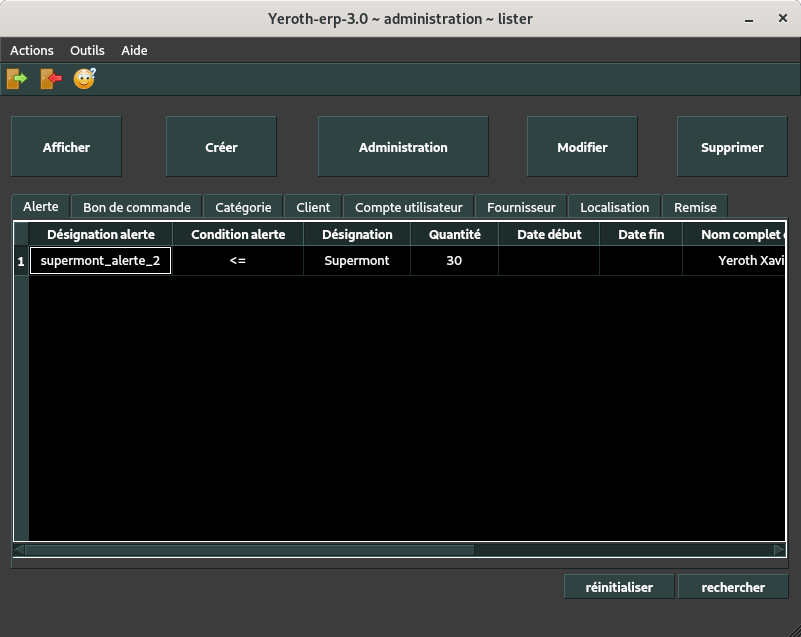
\includegraphics[scale=0.45]{images/alerte-lister.png}
	\caption{L'interface graphique qui liste les alertes.}
	\label{fig:admin-alertes-lister}
\end{figure}

\procparagraph{Proc\'edure pour lister les alertes}
\begin{enumerate}[1)]
	\item \`A partir de l'interface graphique de l'acceuil de
		l'administration (voir la figure~\ref{fig:fenetre-administrateur}),
		on clique sur l'onglet intitul\'e \textbf{op\'erations}. 
		
	\item Choisir '\textbf{lister}' dans le '\emph{combo box
		op\'erations}'.
		
	\item Choisir '\textbf{une alerte}' dans le '\emph{combo box
		sujets}'. Vous \^etes automatiquement conduit \`a la fen\^etre
		qui liste les alertes (voir la figure~\ref{fig:admin-alertes-lister}).
\end{enumerate}

%%%%%%%%%%%%%%%%%%%%%%%%%%%%%%%%%%%%%%%%%%%%%%%%%%%%%%%%%%%%%%%%%%%%%%%%%%%%%%%%%

\newpage
\nxsubsection{Modifier les d\'etails d'une alerte}
\index{modifier les d\'etails d'une alerte}

La figure~\ref{fig:admin-alertes-modifier} illustre
l'interface graphique de \yeroth pour modifier les
d\'etails d'une alerte.\\

\begin{figure}[!htpb]
	\centering
	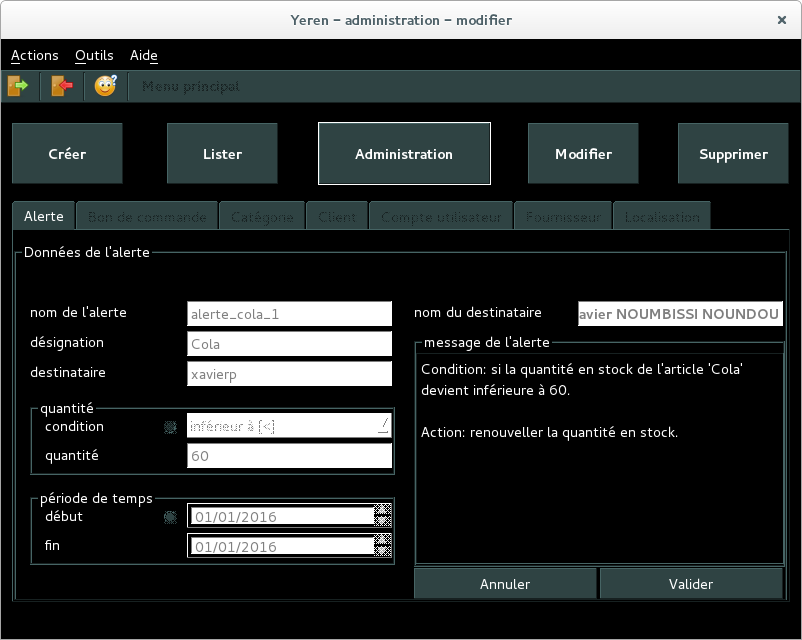
\includegraphics[scale=0.45]{images/alerte-modifier.png}
	\caption{L'interface graphique pour modifier les d'\'etails
	d'une alerte.}\label{fig:admin-alertes-modifier}
\end{figure}

\procparagraph{Proc\'edure pour modifier les d\'etails d'une alerte}
\begin{enumerate}[1)]
	\item \`A partir de l'interface graphique de l'acceuil de
		l'administration (voir figure~\ref{fig:fenetre-administrateur}),
		on clique sur l'onglet intitul\'e \textbf{op\'erations}. 
		
	\item Choisir '\textbf{lister}' dans le '\emph{combo box
		op\'erations}'.
		
	\item Choisir '\textbf{une alerte}' dans le '\emph{combo box
		sujets}'. Vous \^etes automatiquement conduit \`a la fen\^etre
		illustr\'ee par la figure~\ref{fig:admin-alertes-lister}.
		
	\item S\'electionner l'alerte dont vous souhaitez modifier
		les d\'etails dans la liste des alertes affich\'ee.
		
	\item Cliquer sur le bouton \bouton{Modifier}. Les d\'etails
		sur le stock sont affich\'es dans une nouvelle fen\^etre.
		
	\item Faites les modifications que vous souhaitez. Pour
		les alertes, seul le message d'alerte peut \^etre
		modifi\'e.
		
	\item Cliquer sur le bouton \bouton{valider} pour valider
		les modifications faites.
\end{enumerate}

%%%%%%%%%%%%%%%%%%%%%%%%%%%%%%%%%%%%%%%%%%%%%%%%%%%%%%%%%%%%%%%%%%%%%%%%%%%%%%%%%

\newpage
\nxsubsection{Supprimer une alerte}
\index{supprimer une alerte}

La figure~\ref{fig:admin-alertes-supprimer} illustre l'interface
graphique de \yeroth pour supprimer une alerte.\\

\begin{figure}[!htpb]
	\centering
	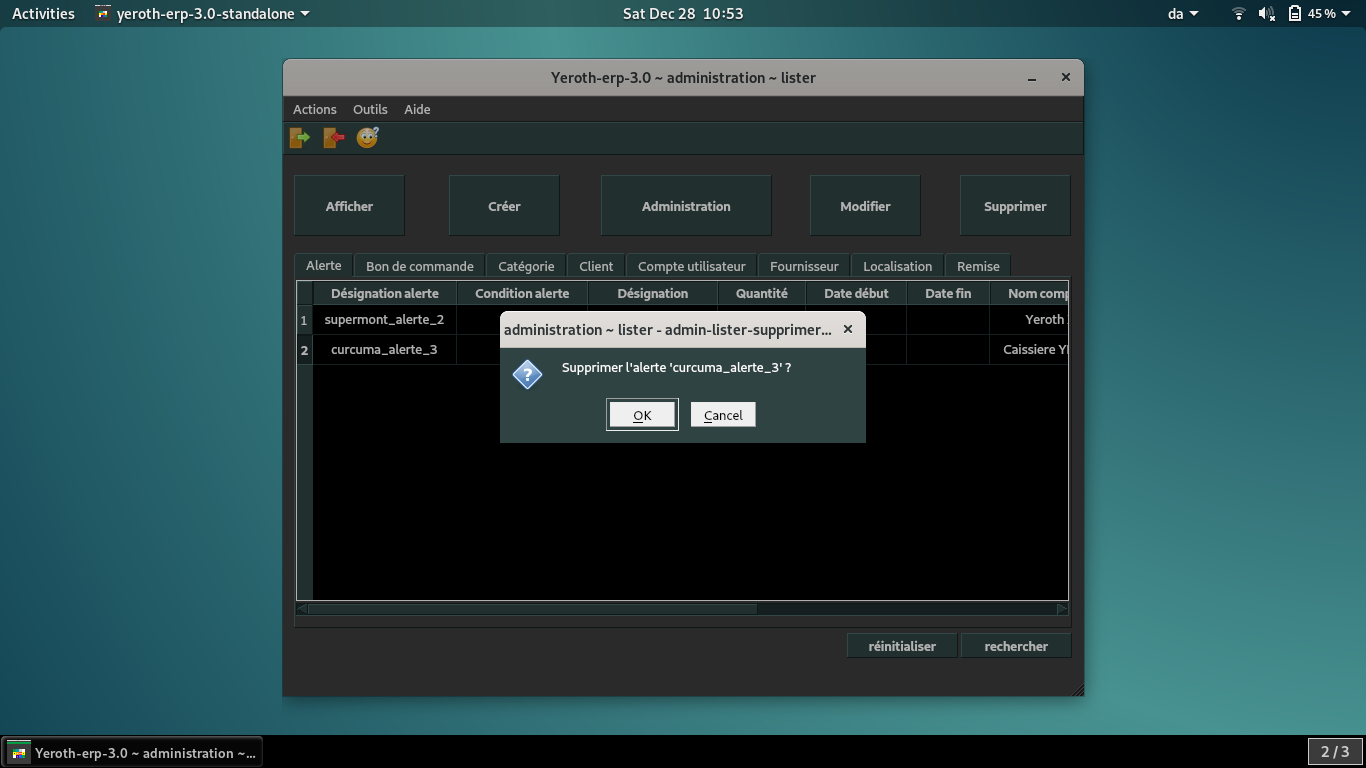
\includegraphics[scale=0.35]{images/alerte-supprimer.png}
	\caption{L'interface graphique pour supprimer des alertes.}
	\label{fig:admin-alertes-supprimer}
\end{figure}

\procparagraph{Proc\'edure pour supprimer une alerte}
\begin{enumerate}[1)]
	\item \`A partir de l'interface graphique de l'acceuil de
		l'administration (voir figure~\ref{fig:fenetre-administrateur}),
		on clique sur l'onglet intitul\'e \textbf{op\'erations}. 
		
	\item Choisir '\textbf{supprimer}' dans le '\emph{combo box
		op\'erations}'.
		
	\item Choisir '\textbf{une alerte}' dans le '\emph{combo box
		sujets}'. Vous \^etes automatiquement conduit \`a la fen\^etre
		illustr\'ee par la figure~\ref{fig:admin-alertes-lister}.
		
	\item S\'electionner l'alerte \`a supprimer dans la liste
		des alertes affich\'ee.
		
	\item Cliquer sur le bouton \bouton{Supprimer}. La question
		est ensuite pos\'ee si vous confirmer votre choix.
		Cliquer sur le \bouton{OK} pour confirmer votre choix.
\end{enumerate}

\newpage

%-----------------------------------------------------------

\nxsection{Les Cat\'egories d'Articles}
\index{les cat\'egories d'articles}

\nxsubsection{Afficher les d\'etails d'une cat\'egorie d'articles}
\index{afficher les d\'etails d'une cat\'egorie d'articles}
\index{d\'etails d'une cat\'egorie d'articles}

\begin{figure}[!htpb]
	\centering
	\includegraphics[scale=0.45]{images/categorie-articles-afficher-details.png}
	\caption{L'interface graphique pour afficher les d\'etails d'une
			cat\'egorie d'articles.}
	\label{fig:admin-categories-articles-afficher-details}
\end{figure}

La figure~\ref{fig:admin-categories-articles-afficher-details}
illustre l'interface graphique de \yeren qui affiche
les d\'etails d'une cat\'egorie d'articles.

\procparagraph{Proc\'edure pour afficher les d\'etails
	d'une cat\'egorie d'articles}
\begin{enumerate}[1)]
	\item \`A partir de l'interface graphique de l'acceuil de
		l'administration (voir figure~\ref{fig:fenetre-administrateur}),
		on clique sur l'onglet intitul\'e \textbf{op\'erations}. 
		
	\item Choisir '\textbf{lister}' dans le '\emph{combo box
		op\'erations}'.
		
	\item Choisir '\textbf{une cat\'egorie d'articles}' dans le
		'\emph{combo box objets}'. Vous \^etes automatiquement
		conduit \`a la fen\^etre illustr\'ee par la
		figure~\ref{fig:admin-categories-articles-lister}.
		
	\item S\'electionner la cat\'egorie d'articles dont vous
		souhaitez afficher les d\'etails.
		
	\item Cliquer sur le bouton \bouton{Afficher}. Les d\'etails
		sur la cat\'egorie d'articles sont affich\'es dans une
		nouvelle fen\^etre.
\end{enumerate}

%%%%%%%%%%%%%%%%%%%%%%%%%%%%%%%%%%%%%%%%%%%%%%%%%%%%%%%%%%%%%%%%%%%%%%%%%%%%%%%%%

\newpage
\nxsubsection{Cr\'eer une cat\'egorie d'articles}
\index{cr\'eer une cat\'egorie d'articles}

\begin{figure}[!htpb]
	\centering
	\includegraphics[scale=0.45]{images/categorie-articles-creer.png}
	\caption{L'interface graphique pour cr\'eer une cat\'egorie d'articles.}
	\label{fig:admin-categories-articles-creer}
\end{figure}

La figure~\ref{fig:admin-categories-articles-creer} illustre
l'interface graphique de \yeren pour cr\'eer une nouvelle
cat\'egorie d'articles.

\procparagraph{Proc\'edure pour cr\'eer une cat\'egorie d'articles}
\begin{enumerate}[1)]
	\item \`A partir de l'interface graphique de l'acceuil de
		l'administration (voir figure~\ref{fig:fenetre-administrateur}),
		on clique sur l'onglet intitul\'e \textbf{op\'erations}. 
		
	\item Choisir '\textbf{cr\'eer}' dans le '\emph{combo box
		op\'erations}'.
		
	\item Choisir '\textbf{une cat\'egorie d'articles}' dans
		le '\emph{combo box objets}'. Vous \^etes automatiquement
		conduit \`a la fen\^etre illustr\'ee par la
		figure~\ref{fig:admin-categories-articles-creer}.
		
	\item Saisissez la d\'esignation de la nouvelle cat\'egorie
		d'articles \`a cr\'eer dans le champs de texte
		'\textbf{d\'esignation}'.

	\item Si vous le souhaitez, saisisser un texte qui d\'ecrit
		cette nouvelle cat\'egorie d'articles dans le champs de
		texte '\textbf{description de la cat\'egorie}'.
		
	\item Cliquer sur le bouton \bouton{Valider} pour
		valider votre travail.		
\end{enumerate}

%%%%%%%%%%%%%%%%%%%%%%%%%%%%%%%%%%%%%%%%%%%%%%%%%%%%%%%%%%%%%%%%%%%%%%%%%%%%%%%%%

\newpage
\nxsubsection{Lister les cat\'egories d'articles}\label{sec:administration-categorie-lister}
\index{lister les cat\'egories d'articles}

\begin{figure}[!htpb]
	\centering
	\includegraphics[scale=0.45]{images/categorie-articles-lister.png}
	\caption{L'interface graphique qui liste les cat\'egories d'articles.}
	\label{fig:admin-categories-articles-lister}
\end{figure}

La figure~\ref{fig:admin-categories-articles-lister} illustre
l'interface graphique de \yeren qui liste les cat\'egories
d'articles.

\procparagraph{Proc\'edure pour lister les cat\'egories d'articles}
\begin{enumerate}[1)]
	\item \`A partir de l'interface graphique de l'acceuil de
		l'administration (voir figure~\ref{fig:fenetre-administrateur}),
		on clique sur l'onglet intitul\'e \textbf{op\'erations}. 
		
	\item Choisir '\textbf{lister}' dans le '\emph{combo box
		op\'erations}'.
		
	\item Choisir '\textbf{une cat\'egorie d'articles}' dans
		le '\emph{combo box objets}'. Vous \^etes automatiquement
		conduit \`a la fen\^etre qui liste les cat\'egories
		d'articles (figure~\ref{fig:admin-categories-articles-lister}).
\end{enumerate}

%%%%%%%%%%%%%%%%%%%%%%%%%%%%%%%%%%%%%%%%%%%%%%%%%%%%%%%%%%%%%%%%%%%%%%%%%%%%%%%%%

\newpage
\nxsubsection{Modifier les d\'etails d'une cat\'egorie d'articles}
\index{modifier les d\'etails d'une cat\'egorie d'articles}

\begin{figure}[!htpb]
	\centering
	\includegraphics[scale=0.45]{images/categorie-articles-modifier.png}
	\caption{L'interface graphique pour modifier les d'\'etails
			d'une cat\'egorie d'articles.}
	\label{fig:admin-categories-articles-modifier}
\end{figure}

La figure~\ref{fig:admin-categories-articles-modifier}
illustre l'interface graphique de \yeren pour modifier
les d\'etails d'une cat\'egorie d'articles.

\procparagraph{Proc\'edure pour modifier les d\'etails
	d'une cat\'egorie d'articles}
\begin{enumerate}[1)]
	\item \`A partir de l'interface graphique de l'acceuil de
		l'administration (voir figure~\ref{fig:fenetre-administrateur}),
		on clique sur l'onglet intitul\'e \textbf{op\'erations}. 
		
	\item Choisir '\textbf{lister}' dans le '\emph{combo box
		op\'erations}'.
		
	\item Choisir '\textbf{cat\'egorie d'articles}' dans le
		'\emph{combo box objets}'. Vous \^etes automatiquement
		conduit \`a la fen\^etre illustr\'ee par la
		figure~\ref{fig:admin-categories-articles-lister}.
		
	\item S\'electionner l'alerte dont vous souhaitez modifier
		les d\'etails dans la liste	des d\'esignations des
		cat\'egories d'articles affich\'ee.
		
	\item Cliquer sur le bouton \bouton{Modifier}. Les d\'etails
		sur le stock sont affich\'es dans une nouvelle fen\^etre.
		
	\item Faites les modifications que vous souhaitez. Pour
		les alertes, seul le message d'alerte peut \^etre
		modifi\'e.
		
	\item Cliquer sur le bouton \bouton{valider} pour valider
		les modifications faites.
\end{enumerate}

%%%%%%%%%%%%%%%%%%%%%%%%%%%%%%%%%%%%%%%%%%%%%%%%%%%%%%%%%%%%%%%%%%%%%%%%%%%%%%%%%

\newpage
\nxsubsection{Supprimer une cat\'egorie d'article}
\index{supprimer une cat\'egorie d'article}

\begin{figure}[!htpb]
	\centering
	\includegraphics[scale=0.39]{images/categorie-articles-supprimer.png}
	\caption{L'interface graphique pour supprimer une cat\'egorie d'articles.}
	\label{fig:admin-categories-articles-supprimer}
\end{figure}

La figure~\ref{fig:admin-categories-articles-supprimer} illustre
l'interface graphique de \yeren pour supprimer une
cat\'egorie d'articles.

\procparagraph{Proc\'edure pour supprimer une cat\'egorie d'articles}
\begin{enumerate}[1)]
	\item \`A partir de l'interface graphique de l'acceuil de
		l'administration (voir figure~\ref{fig:fenetre-administrateur}),
		on clique sur l'onglet intitul\'e \textbf{op\'erations}. 
		
	\item Choisir '\textbf{supprimer}' dans le '\emph{combo box
		op\'erations}'.
		
	\item Choisir '\textbf{une cat\'egorie d'articles}' dans le
		'\emph{combo box objets}'. Vous \^etes automatiquement
		conduit \`a la fen\^etre illustr\'ee par la
		figure~\ref{fig:admin-categories-articles-lister}.
		
	\item S\'electionner l'alerte \`a supprimer dans la liste
		des d\'esignations des cat\'egories d'articles affich\'ee.
		
	\item Cliquer sur le bouton \bouton{Supprimer}. La question
		est ensuite pos\'ee si vous confirmer votre choix.
		Cliquer sur le \bouton{OK} pour confirmer votre choix.
\end{enumerate}

\newpage

%-----------------------------------------------------------

\nxsection{Les Comptes Clients}
\index{les comptes clients}

\nxsubsection{Afficher les d\'etails d'un compte client}
\index{afficher les d\'etails d'un compte client}

\begin{figure}[!htpb]
	\centering
	\includegraphics[scale=0.45]{images/compte-client-afficher-details.png}
	\caption{L'interface graphique pour afficher les d\'etails d'un compte client.}
	\label{fig:admin-compte-client-afficher-details}
\end{figure}

La figure~\ref{fig:admin-compte-client-afficher-details}
illustre l'interface graphique de \yeren qui affiche les
d\'etails d'un compte client.

\procparagraph{Proc\'edure pour afficher les d\'etails d'un compte client}
\begin{enumerate}[1)]
	\item \`A partir de l'interface graphique de l'acceuil de
		l'administration (voir figure~\ref{fig:fenetre-administrateur}),
		on clique sur l'onglet intitul\'e \textbf{op\'erations}. 
		
	\item Choisir '\textbf{lister}' dans le '\emph{combo box
		op\'erations}'.
		
	\item Choisir '\textbf{un compte client}' dans le '\emph{combo box
		sujets}'. Vous \^etes automatiquement conduit \`a la fen\^etre
		illustr\'ee par la figure~\ref{fig:admin-comptes-clients-lister}.
		
	\item S\'electionner le compte client dont vous souhaitez afficher
		les d\'etails dans la liste des comptes clients affich\'ee.
		
	\item Cliquer sur le bouton \bouton{Afficher}. Les d\'etails
		du compte client sont affich\'es dans une nouvelle fen\^etre.
\end{enumerate}

%------------------------------------------------------------------------------

\newpage
\nxsubsection{Cr\'eer un compte client}\label{sec:administration-comptes-clients-lister}
\index{cr\'eer un compte client}

\begin{figure}[!htpb]
	\centering
	\includegraphics[scale=0.45]{images/compte-client-creer.png}
	\caption{L'interface graphique pour cr\'eer un compte client.}
	\label{fig:admin-comptes-clients-creer}
\end{figure}

La figure~\ref{fig:admin-comptes-clients-creer} illustre
l'interface graphique de \yeren pour cr\'eer un nouveau
compte client.

\procparagraph{Proc\'edure pour cr\'eer un compte client}
\begin{enumerate}[1)]
	\item \`A partir de l'interface graphique de l'acceuil de
		l'administration (voir figure~\ref{fig:fenetre-administrateur}),
		on clique sur l'onglet intitul\'e \textbf{op\'erations}. 
		
	\item Choisir '\textbf{cr\'eer}' dans le '\emph{combo box
		op\'erations}'.
		
	\item Choisir '\textbf{un compte client}' dans
		le '\emph{combo box objets}'. Vous \^etes automatiquement
		conduit \`a la fen\^etre illustr\'ee par la
		figure~\ref{fig:admin-comptes-clients-creer}.
		
	\item Saisissez les informations requises dans les champs de texte
		suivants:
		\begin{enumerate}[1)]
			\item nom de l'entreprise \obligatoire
			\item nom du r\'epr\'esentant \obligatoire
			\item quartier
			\item ville 
			\item pays
			\item si\`ege social 
			\item \'email@ 
			\item num\'ero de t\'el\'ephone 1 
			\item num\'ero de t\'el\'ephone 2
			\item num\'ero de contribuable 
			\item description du client.			
		\end{enumerate}
		
	\item Cliquer sur le bouton \bouton{Valider} pour
		valider votre travail.		
\end{enumerate}

%------------------------------------------------------------------------------

\newpage
\nxsubsection{Lister les comptes clients}\label{sec:administration-comptes-clients-lister}
\index{lister les comptes clients}

\begin{figure}[!htpb]
	\centering
	\includegraphics[scale=0.45]{images/compte-client-lister.png}
	\caption{L'interface graphique qui liste les comptes clients.}
	\label{fig:admin-comptes-clients-lister}
\end{figure}

La figure~\ref{fig:admin-comptes-clients-lister} illustre
l'interface graphique de \yeren qui liste les comptes clients.

\procparagraph{Proc\'edure pour lister les comptes clients}
\begin{enumerate}[1)]
	\item \`A partir de l'interface graphique de l'acceuil de
		l'administration (voir figure~\ref{fig:fenetre-administrateur}),
		on clique sur l'onglet intitul\'e \textbf{op\'erations}. 
		
	\item Choisir '\textbf{lister}' dans le '\emph{combo box
		op\'erations}'.
		
	\item Choisir '\textbf{un compte client}' dans
		le '\emph{combo box objets}'. Vous \^etes automatiquement
		conduit \`a la fen\^etre qui liste les comptes clients
		(figure~\ref{fig:admin-comptes-clients-lister}).
\end{enumerate}

%------------------------------------------------------------------------------

\newpage
\nxsubsection{Modifier les d\'etails d'un compte client}
\index{modifier les d\'etails d'un compte client}

\begin{figure}[!htpb]
	\centering
	\includegraphics[scale=0.45]{images/compte-client-modifier.png}
	\caption{L'interface graphique pour modifier les d\'etails
			d'un compte client.}
	\label{fig:admin-comptes-clients-modifier}
\end{figure}

La figure~\ref{fig:admin-comptes-clients-modifier} illustre
l'interface graphique de \yeren pour modifier les
d\'etails d'un compte client.

\procparagraph{Proc\'edure pour modifier les d\'etails d'un compte client}
\begin{enumerate}[1)]
	\item \`A partir de l'interface graphique de l'acceuil de
		l'administration (voir figure~\ref{fig:fenetre-administrateur}),
		on clique sur l'onglet intitul\'e \textbf{op\'erations}. 
		
	\item Choisir '\textbf{lister}' dans le '\emph{combo box
		op\'erations}'.
		
	\item Choisir '\textbf{un compte client}' dans le '\emph{combo box
		sujets}'. Vous \^etes automatiquement conduit \`a la fen\^etre
		illustr\'ee par la figure~\ref{fig:admin-comptes-clients-lister}.
		
	\item S\'electionner le compte client dont vous souhaitez
		modifier les d\'etails dans la liste des comptes
		clients affich\'ee.
		
	\item Cliquer sur le bouton \bouton{Modifier}. Les d\'etails
		du compte client sont affich\'es dans une nouvelle fen\^etre.
		
	\item Faites les modifications que vous souhaitez.
		
	\item Cliquer sur le bouton \bouton{valider} pour valider
		les modifications faites.
\end{enumerate}

%------------------------------------------------------------------------------

\newpage
\nxsubsection{Supprimer un compte client}
\index{supprimer un compte client}

\begin{figure}[!htpb]
	\centering
	\includegraphics[scale=0.39]{images/compte-client-supprimer.png}
	\caption{L'interface graphique pour supprimer un compte client.}
	\label{fig:admin-comptes-clients-supprimer}
\end{figure}

La figure~\ref{fig:admin-comptes-clients-supprimer} illustre
l'interface graphique de \yeren pour supprimer un compte
client.

\procparagraph{Proc\'edure pour supprimer un compte client}
\begin{enumerate}[1)]
	\item \`A partir de l'interface graphique de l'acceuil de
		l'administration (voir figure~\ref{fig:fenetre-administrateur}),
		on clique sur l'onglet intitul\'e \textbf{op\'erations}. 
		
	\item Choisir '\textbf{supprimer}' dans le '\emph{combo box
		op\'erations}'.
		
	\item Choisir '\textbf{un compte client}' dans le '\emph{combo box
		sujets}'. Vous \^etes automatiquement conduit \`a la fen\^etre
		illustr\'ee par la figure~\ref{fig:admin-comptes-clients-lister}.
		
	\item S\'electionner le compte client \`a supprimer dans la liste
		des comptes clients affich\'ee.
		
	\item Cliquer sur le bouton \bouton{Supprimer}. La question
		est ensuite pos\'ee si vous confirmer votre choix.
		Cliquer sur le \bouton{OK} pour confirmer votre choix.
\end{enumerate}

\newpage

%-----------------------------------------------------------

\nxsection{Les Comptes Fournisseurs}
\index{les comptes fournisseurs}

\nxsubsection{Afficher les d\'etails d'un compte fournisseur}
\index{afficher les d\'etails d'un compte fournisseur}
\index{d\'etails d'un compte fournisseur}

\begin{figure}[!htpb]
	\centering
	\includegraphics[scale=0.45]{images/compte-fournisseur-afficher-details.png}
	\caption{L'interface graphique pour afficher les d\'etails
			d'un compte fournisseur.}
	\label{fig:admin-fournisseurs-afficher-details}
\end{figure}

La figure~\ref{fig:admin-fournisseurs-afficher-details}
illustre l'interface graphique de \yeroth qui affiche
les d\'etails d'un compte fournisseur.

\procparagraph{Proc\'edure pour afficher les d\'etails
	d'un compte fournisseur}
\begin{enumerate}[1)]
	\item \`A partir de l'interface graphique de l'acceuil de
		l'administration (voir figure~\ref{fig:fenetre-administrateur}),
		on clique sur l'onglet intitul\'e \textbf{op\'erations}. 
		
	\item Choisir '\textbf{lister}' dans le '\emph{combo box
		op\'erations}'.
		
	\item Choisir '\textbf{un compte fournisseur}' dans le
		'\emph{combo box objets}'. Vous \^etes automatiquement
		conduit \`a la fen\^etre illustr\'ee par la
		figure~\ref{fig:admin-comptes-fournisseurs-lister}.
		
	\item S\'electionner le compte fournisseur dont vous
		souhaitez afficher les d\'etails dans la liste des
		comptes fournisseurs affich\'ee.
		
	\item Cliquer sur le bouton \bouton{Afficher}. Les d\'etails
		sur le compte fournisseur sont affich\'es dans une nouvelle.
\end{enumerate}

%%%%%%%%%%%%%%%%%%%%%%%%%%%%%%%%%%%%%%%%%%%%%%%%%%%%%%%%%%%%%%%%%%%%%%%%%%%%%%%%%

\newpage
\nxsubsection{Cr\'eer un compte fournisseur}
\index{cr\'eer un compte fournisseur}

\begin{figure}[!htpb]
	\centering
	\includegraphics[scale=0.45]{images/compte-fournisseur-creer.png}
	\caption{L'interface graphique pour cr\'eer un
			nouveau compte fournisseur.}
	\label{fig:admin-comptes-fournisseurs-creer}
\end{figure}

La figure~\ref{fig:admin-comptes-fournisseurs-creer} illustre
l'interface graphique de \yeroth pour cr\'eer un nouveau
compte fournisseur.

\procparagraph{Proc\'edure pour cr\'eer un compte fournisseur}
\begin{enumerate}[1)]
	\item \`A partir de l'interface graphique de l'acceuil de
		l'administration (voir figure~\ref{fig:fenetre-administrateur}),
		on clique sur l'onglet intitul\'e \textbf{op\'erations}. 
		
	\item Choisir '\textbf{cr\'eer}' dans le '\emph{combo box
		op\'erations}'.
		
	\item Choisir '\textbf{un compte fournisseur}' dans
		le '\emph{combo box objets}'. Vous \^etes automatiquement
		conduit \`a la fen\^etre illustr\'ee par la
		figure~\ref{fig:admin-comptes-fournisseurs-creer}.
		
	\item Saisissez les informations requises dans les champs de texte
		suivants:
		\begin{enumerate}[1)]
			\item nom de l'entreprise \obligatoire
			\item nom du r\'epr\'esentant
			\item quartier
			\item ville 
			\item pays
			\item si\`ege social
			\item \'email@
			\item num\'ero de t\'el\'ephone 1
			\item num\'ero de t\'el\'ephone 2
			\item num\'ero de contribuable 
			\item description du fournisseur.
		\end{enumerate}
		
	\item Cliquer sur le bouton \bouton{Valider} pour
		valider votre travail.		
\end{enumerate}

%%%%%%%%%%%%%%%%%%%%%%%%%%%%%%%%%%%%%%%%%%%%%%%%%%%%%%%%%%%%%%%%%%%%%%%%%%%%%%%%%

\newpage
\nxsubsection{Lister les fournisseurs}
\index{lister les fournisseurs}

\begin{figure}[!htpb]
	\centering
	\includegraphics[scale=0.45]{images/compte-fournisseur-lister.png}
	\caption{L'interface graphique pour lister les comptes fournisseurs.}
	\label{fig:admin-comptes-fournisseurs-lister}
\end{figure}

La figure~\ref{fig:admin-comptes-fournisseurs-lister} illustre
l'interface graphique de \yeroth qui liste les comptes fournisseurs.

\procparagraph{Proc\'edure pour lister les comptes fournisseurs}
\begin{enumerate}[1)]
	\item \`A partir de l'interface graphique de l'acceuil de
		l'administration (voir figure~\ref{fig:fenetre-administrateur}),
		on clique sur l'onglet intitul\'e \textbf{op\'erations}. 
		
	\item Choisir '\textbf{lister}' dans le '\emph{combo box
		op\'erations}'.
		
	\item Choisir '\textbf{un compte fournisseur}' dans
		le '\emph{combo box objets}'. Vous \^etes automatiquement
		conduit \`a la fen\^etre qui liste les comptes fournisseurs
		(figure~\ref{fig:admin-comptes-fournisseurs-lister}).
\end{enumerate}

%%%%%%%%%%%%%%%%%%%%%%%%%%%%%%%%%%%%%%%%%%%%%%%%%%%%%%%%%%%%%%%%%%%%%%%%%%%%%%%%%

\newpage
\nxsubsection{Modifier les d\'etails d'un fournisseur}
\index{modifier les d\'etails d'un fournisseur}

\begin{figure}[!htpb]
	\centering
	\includegraphics[scale=0.45]{images/compte-fournisseur-modifier.png}
	\caption{L'interface graphique pour modifier les
			d\'etails d'un compte fournisseur.}
	\label{fig:admin-comptes-fournisseurs-modifier}
\end{figure}

La figure~\ref{fig:admin-comptes-fournisseurs-modifier} illustre
l'interface graphique de \yeroth pour modifier les
d\'etails d'un compte fournisseur.

\procparagraph{Proc\'edure pour modifier les d\'etails d'un compte fournisseur}
\begin{enumerate}[1)]
	\item \`A partir de l'interface graphique de l'acceuil de
		l'administration (voir figure~\ref{fig:fenetre-administrateur}),
		on clique sur l'onglet intitul\'e \textbf{op\'erations}. 
		
	\item Choisir '\textbf{lister}' dans le '\emph{combo box
		op\'erations}'.
		
	\item Choisir '\textbf{un compte fournisseur}' dans le '\emph{combo box
		sujets}'. Vous \^etes automatiquement conduit \`a la fen\^etre
		illustr\'ee par la figure~\ref{fig:admin-comptes-fournisseurs-lister}.
		
	\item S\'electionner le compte fournisseur dont vous souhaitez
		modifier les d\'etails dans la liste des comptes fournisseurs
		affich\'ee.
		
	\item Cliquer sur le bouton \bouton{Modifier}. Les d\'etails
		du compte fournisseur sont affich\'es dans une nouvelle fen\^etre.
		
	\item Faites les modifications que vous souhaitez.
		
	\item Cliquer sur le bouton \bouton{valider} pour valider
		les modifications faites.
\end{enumerate}

%%%%%%%%%%%%%%%%%%%%%%%%%%%%%%%%%%%%%%%%%%%%%%%%%%%%%%%%%%%%%%%%%%%%%%%%%%%%%%%%%

\newpage
\nxsubsection{Supprimer un compte fournisseur}
\index{supprimer un compte fournisseur}

\begin{figure}[!htpb]
	\centering
	\includegraphics[scale=0.39]{images/compte-fournisseur-supprimer.png}
	\caption{L'interface graphique pour supprimer un fournisseur.}
	\label{fig:admin-comptes-fournisseurs-supprimer}
\end{figure}

La figure~\ref{fig:admin-comptes-fournisseurs-supprimer}
illustre l'interface graphique de \yeroth pour supprimer
un compte fournisseur.

\procparagraph{Proc\'edure pour supprimer un compte fournisseur}
\begin{enumerate}[1)]
	\item \`A partir de l'interface graphique de l'acceuil de
		l'administration (voir figure~\ref{fig:fenetre-administrateur}),
		on clique sur l'onglet intitul\'e \textbf{op\'erations}. 
		
	\item Choisir '\textbf{supprimer}' dans le '\emph{combo box
		op\'erations}'.
		
	\item Choisir '\textbf{un compte fournisseur}' dans le
		'\emph{combo box objets}'. Vous \^etes automatiquement
		conduit \`a la fen\^etre illustr\'ee par la
		figure~\ref{fig:admin-comptes-fournisseurs-lister}.
		
	\item S\'electionner le compte fournisseur \`a supprimer
		dans la liste des comptes fournisseurs affich\'ee.
		
	\item Cliquer sur le bouton \bouton{Supprimer}. La question
		est ensuite pos\'ee si vous confirmer votre choix.
		Cliquer sur le \bouton{OK} pour confirmer votre choix.
\end{enumerate}

\newpage

%-----------------------------------------------------------

\nxsection{Les Comptes Utilisateurs}
\index{les comptes utilisateurs}

\nxsubsection{Afficher les d\'etails d'un compte utilisateur}
\index{afficher les d\'etails d'un compte utilisateur}
\index{d\'etails d'un compte utilisateur}

\begin{figure}[!htpb]
	\centering
	\includegraphics[scale=0.45]{images/compte-utilisateur-afficher-details.png}
	\caption{L'interface graphique pour afficher les d\'etails
			d'un compte utilisateur.}
	\label{fig:admin-comptes-utilisateurs-afficher-details}
\end{figure}

La figure~\ref{fig:admin-comptes-utilisateurs-afficher-details}
illustre l'interface graphique de \yeroth qui affiche les
d\'etails d'un compte utilisateur.

\procparagraph{Proc\'edure pour afficher les d\'etails d'un compte utilisateur}
\begin{enumerate}[1)]
	\item \`A partir de l'interface graphique de l'acceuil de
		l'administration (voir figure~\ref{fig:fenetre-administrateur}),
		on clique sur l'onglet intitul\'e \textbf{op\'erations}. 
		
	\item Choisir '\textbf{lister}' dans le '\emph{combo box
		op\'erations}'.
		
	\item Choisir '\textbf{un compte utilisateur}' dans le
		'\emph{combo box objets}'. Vous \^etes automatiquement
		conduit \`a la fen\^etre illustr\'ee par la
		figure~\ref{fig:admin-comptes-utilisateurs-lister}.
		
	\item S\'electionner le compte utilisateur dont vous
		souhaitez afficher les d\'etails dans la liste des
		comptes utilisateurs affich\'ee.
		
	\item Cliquer sur le bouton \bouton{Afficher}. Les d\'etails
		sur le compte utilisateur sont affich\'es dans
		une nouvelle fen\^etre.
\end{enumerate}

%%%%%%%%%%%%%%%%%%%%%%%%%%%%%%%%%%%%%%%%%%%%%%%%%%%%%%%%%%%%%%%%%%%%%%%%%%%%%%%%%

\newpage
\nxsubsection{Cr\'eer un compte utilisateur}
\index{cr\'eer un compte utilisateur}

\begin{figure}[!htpb]
	\centering
	\includegraphics[scale=0.45]{images/compte-utilisateur-creer.png}
	\caption{L'interface graphique pour cr\'eer un compte utilisateur.}
	\label{fig:admin-comptes-utilisateurs-creer}
\end{figure}

La figure~\ref{fig:admin-comptes-utilisateurs-creer} illustre
l'interface graphique de \yeroth pour cr\'eer un nouveau
compte utilisateur.

\procparagraph{Proc\'edure pour cr\'eer un compte utilisateur}
\begin{enumerate}[1)]
	\item \`A partir de l'interface graphique de l'acceuil de
		l'administration (voir figure~\ref{fig:fenetre-administrateur}),
		on clique sur l'onglet intitul\'e \textbf{op\'erations}. 
		
	\item Choisir '\textbf{cr\'eer}' dans le '\emph{combo box
		op\'erations}'.
		
	\item Choisir '\textbf{un compte utilisateur}' dans
		le '\emph{combo box objets}'. Vous \^etes automatiquement
		conduit \`a la fen\^etre illustr\'ee par la
		figure~\ref{fig:admin-comptes-utilisateurs-creer}.
		
	\item Saisissez les informations requises dans les champs
		de texte suivants:
		\begin{enumerate}[1)]
			\item pr\'enoms \obligatoire
			\item noms \obligatoire
			\item titre	\obligatoire
			\item lieu de naissance 
			\item date de naissance
			\item ville
			\item province / \'etat
			\item pays
			\item bo\^ite postale
			\item \'email 
			\item num\'ero de t\'el\'ephone 1 
			\item num\'ero de t\'el\'ephone 2 
			\item nom d'utilisateur \obligatoire
			\item mot de passe \obligatoire
			\item v\'erification du mot de passe \obligatoire			
			\item r\^ole \obligatoire.
		\end{enumerate}
		
	\item Cliquer sur le bouton \bouton{Valider} pour
		valider votre travail.	
\end{enumerate}


%%%%%%%%%%%%%%%%%%%%%%%%%%%%%%%%%%%%%%%%%%%%%%%%%%%%%%%%%%%%%%%%%%%%%%%%%%%%%%%%%

\newpage
\nxsubsection{Lister les comptes utilisateurs}
\index{lister les comptes utilisateur}

\begin{figure}[!htpb]
	\centering
	\includegraphics[scale=0.45]{images/compte-utilisateur-lister.png}
	\caption{L'interface graphique pour lister les comptes utilisateurs.}
	\label{fig:admin-comptes-utilisateurs-lister}
\end{figure}

La figure~\ref{fig:admin-comptes-utilisateurs-lister}
illustre l'interface graphique de \yeroth qui liste les
comptes utilisateurs.

\procparagraph{Proc\'edure pour lister les comptes utilisateurs}
\begin{enumerate}[1)]
	\item \`A partir de l'interface graphique de l'acceuil de
		l'administration (voir figure~\ref{fig:fenetre-administrateur}),
		on clique sur l'onglet intitul\'e \textbf{op\'erations}. 
		
	\item Choisir '\textbf{lister}' dans le '\emph{combo box
		op\'erations}'.
		
	\item Choisir '\textbf{un compte utilisateur}' dans
		le '\emph{combo box objets}'. Vous \^etes automatiquement
		conduit \`a la fen\^etre qui liste les comptes clients
		(figure~\ref{fig:admin-comptes-utilisateurs-lister}).
\end{enumerate}

%%%%%%%%%%%%%%%%%%%%%%%%%%%%%%%%%%%%%%%%%%%%%%%%%%%%%%%%%%%%%%%%%%%%%%%%%%%%%%%%%

\newpage
\nxsubsection{Modifier les d\'etails d'un compte utilisateur}
\index{modifier les d\'etails d'un compte utilisateur}

\begin{figure}[!htpb]
	\centering
	\includegraphics[scale=0.45]{images/compte-utilisateur-modifier.png}
	\caption{L'interface graphique pour modifier les d\'etails
			d'un compte utilisateur.}
	\label{fig:admin-comptes-utilisateurs-modifier}
\end{figure}

La figure~\ref{fig:admin-comptes-utilisateurs-modifier} illustre
l'interface graphique de \yeroth pour modifier les d\'etails
d'un compte utilisateur.

\procparagraph{Proc\'edure pour modifier les d\'etails d'un compte utilisateur}
\begin{enumerate}[1)]
	\item \`A partir de l'interface graphique de l'acceuil de
		l'administration (voir figure~\ref{fig:fenetre-administrateur}),
		on clique sur l'onglet intitul\'e \textbf{op\'erations}. 
		
	\item Choisir '\textbf{lister}' dans le '\emph{combo box
		op\'erations}'.
		
	\item Choisir '\textbf{un compte utilisateur}' dans
		le '\emph{combo box objets}'. Vous \^etes automatiquement
		conduit \`a la fen\^etre illustr\'ee par la
		figure~\ref{fig:admin-comptes-utilisateurs-lister}.
		
	\item S\'electionner le compte utilisateur dont vous souhaitez
		modifier les d\'etails dans la liste des comptes
		utilisateurs affich\'ee.
		
	\item Cliquer sur le bouton \bouton{Modifier}. Les d\'etails
		du compte utilisateur sont affich\'es dans une nouvelle fen\^etre.
		
	\item Faites les modifications que vous souhaitez.
		
	\item Cliquer sur le bouton \bouton{valider} pour valider
		les modifications faites.
\end{enumerate}

%%%%%%%%%%%%%%%%%%%%%%%%%%%%%%%%%%%%%%%%%%%%%%%%%%%%%%%%%%%%%%%%%%%%%%%%%%%%%%%%%

\newpage
\nxsubsection{Supprimer un compte utilisateur}
\index{supprimer un compte utilisateur}

\begin{figure}[!htpb]
	\centering
	\includegraphics[scale=0.39]{images/compte-utilisateur-supprimer.png}
	\caption{L'interface graphique pour supprimer un compte utilisateur.}
	\label{fig:admin-comptes-utilisateurs-supprimer}
\end{figure}

La figure~\ref{fig:admin-comptes-utilisateurs-supprimer}
illustre l'interface graphique de \yeroth pour supprimer
un compte utilisateur.

\procparagraph{Proc\'edure pour supprimer un compte utilisateur}
\begin{enumerate}[1)]
	\item \`A partir de l'interface graphique de l'acceuil de
		l'administration (voir figure~\ref{fig:fenetre-administrateur}),
		on clique sur l'onglet intitul\'e \textbf{op\'erations}. 
		
	\item Choisir '\textbf{supprimer}' dans le '\emph{combo box
		op\'erations}'.
		
	\item Choisir '\textbf{un compte utilisateur}' dans le
		'\emph{combo box objets}'. Vous \^etes automatiquement
		conduit \`a la fen\^etre illustr\'ee par la
		figure~\ref{fig:admin-comptes-utilisateurs-lister}.
		
	\item S\'electionner le compte utilisateur \`a supprimer
		dans la liste des comptes utilisateurs affich\'ee.
		
	\item Cliquer sur le bouton \bouton{Supprimer}. La question
		est ensuite pos\'ee si vous confirmer votre choix.
		Cliquer sur le \bouton{OK} pour confirmer votre choix.
\end{enumerate}

\newpage

%-----------------------------------------------------------

\nxsection{Les Localisations}
\index{localisation}

Une localisation repr\'esente une boutique ou un d\'ep\^ot
de l'entreprise utilisant \yeren.

Les informations sur une localisation permettent de
se connecter \`a la base de donn\'ees de la boutique
ou du d\'ep\^ot qu'elle repr\'esente.

\nxsubsection{Afficher les d\'etails d'une localisation}
\index{afficher les d\'etails d'une localisation}
\index{d\'etails d'une localisation}

La figure~\ref{fig:admin-localisations-afficher-details} illustre
l'interface graphique de \yeren qui affiche les d\'etails
d'une localisation.\\

\begin{figure}[!htpb]
	\centering
	\includegraphics[scale=0.45]{images/localisation-afficher-details.png}
	\caption{L'interface graphique pour afficher les d\'etails
			d'une localisation.}
	\label{fig:admin-localisations-afficher-details}
\end{figure}

\procparagraph{Proc\'edure pour afficher les d\'etails d'une localisation}
\begin{enumerate}[1)]
	\item \`A partir de l'interface graphique de l'acceuil de
		l'administration (voir figure~\ref{fig:fenetre-administrateur}),
		on clique sur l'onglet intitul\'e \textbf{op\'erations}. 
		
	\item Choisir '\textbf{lister}' dans le '\emph{combo box
		op\'erations}'.
		
	\item Choisir '\textbf{une localisation}' dans le '\emph{combo box
		sujets}'. Vous \^etes automatiquement conduit \`a la fen\^etre
		illustr\'ee par la figure~\ref{fig:admin-localisations-lister}.
		
	\item S\'electionner la localisation dont vous souhaitez afficher
		les d\'etails dans la liste des localisations affich\'ee.
		
	\item Cliquer sur le bouton \bouton{Afficher}. Les d\'etails
		sur la localisation choisie sont affich\'es dans
		une nouvelle fen\^etre.
\end{enumerate}

%%%%%%%%%%%%%%%%%%%%%%%%%%%%%%%%%%%%%%%%%%%%%%%%%%%%%%%%%%%%%%%%%%%%%%%%%%%%%%%%%

\nxsubsection{Cr\'eer une localisation}
\index{cr\'eer une localisation}

La figure~\ref{fig:admin-localisations-creer} illustre
l'interface graphique de \yeren pour cr\'eer une localisation.\\

\begin{figure}[!htpb]
	\centering
	\includegraphics[scale=0.45]{images/localisation-creer.png}
	\caption{L'interface graphique pour cr\'eer une localisation.}
	\label{fig:admin-localisations-creer}
\end{figure}

\procparagraph{Proc\'edure pour cr\'eer une localisation}
\begin{enumerate}[1)]
	\item \`A partir de l'interface graphique de l'acceuil de
		l'administration (voir figure~\ref{fig:fenetre-administrateur}),
		on clique sur l'onglet intitul\'e \textbf{op\'erations}. 
		
	\item Choisir '\textbf{cr\'eer}' dans le '\emph{combo box
		op\'erations}'.
		
	\item Choisir '\textbf{une localisation}' dans
		le '\emph{combo box objets}'. Vous \^etes automatiquement
		conduit \`a la fen\^etre illustr\'ee par la
		figure~\ref{fig:admin-localisations-creer}.
		
	\item Saisissez les informations requises dans les champs
		de texte suivants:
		\begin{enumerate}[1)]
			\item adresse IP 
			\item nom \obligatoire
			\item num\'ero unique 
			\item quartier
			\item ville
			\item province / \'etat
			\item pays
			\item bo\^ite postale
			\item date d'ouverture
			\item \'email@
			\item num\'ero de t\'el\'ephone 1
			\item num\'ero de t\'el\'ephone 2	
			\item base de donn\'ees					
			\item description du lieu.\\
		\end{enumerate}
		
		Si vous avez entr\'e une adresse IP pour cette 
		localisation, vous devez choisir le type de base de
		donn\'ees utilis\'e dans cette localisation. Pour
		l'instant, \yeren ne fonctionne qu'avec \emphbf{MySQL}.\\
		
		La section~\ref{sec:yeren-sgbd} dans
		l'annexe~\ref{chap:environement-logiciel-requis}
		(L'Environnement Logiciel) contient plus d'information
		aux sujets des bases de donn\'ees dans \yeren.
		
	\item Cliquer sur le bouton \bouton{Valider} pour
		valider votre travail.	
\end{enumerate}

%%%%%%%%%%%%%%%%%%%%%%%%%%%%%%%%%%%%%%%%%%%%%%%%%%%%%%%%%%%%%%%%%%%%%%%%%%%%%%%%%

\newpage
\nxsubsection{Lister les localisations}
\index{lister les localisations}

La figure~\ref{fig:admin-localisations-lister} illustre
l'interface graphique de \yeren qui liste les localisations.\\

\begin{figure}[!htpb]
	\centering
	\includegraphics[scale=0.45]{images/localisation-lister.png}
	\caption{L'interface graphique pour cr\'eer une localisation.}
	\label{fig:admin-localisations-lister}
\end{figure}

\procparagraph{Proc\'edure pour lister les localisations}
\begin{enumerate}[1)]
	\item \`A partir de l'interface graphique de l'acceuil de
		l'administration (voir figure~\ref{fig:fenetre-administrateur}),
		on clique sur l'onglet intitul\'e \textbf{op\'erations}. 
		
	\item Choisir '\textbf{lister}' dans le '\emph{combo box
		op\'erations}'.
		
	\item Choisir '\textbf{une localisation}' dans le
		'\emph{combo box objets}'. Vous \^etes automatiquement
		conduit \`a la fen\^etre qui liste localisations
		(figure~\ref{fig:admin-localisations-lister}).
\end{enumerate}

%%%%%%%%%%%%%%%%%%%%%%%%%%%%%%%%%%%%%%%%%%%%%%%%%%%%%%%%%%%%%%%%%%%%%%%%%%%%%%%%%

\newpage
\nxsubsection{Modifier les d\'etails d'une localisation}
\index{modifier les d\'etails d'une localisation}

La figure~\ref{fig:admin-localisations-modifier} illustre
l'interface graphique de \yeren pour modifier les d\'etails
d'une localisation.\\

\begin{figure}[!htpb]
	\centering
	\includegraphics[scale=0.45]{images/localisation-modifier.png}
	\caption{L'interface graphique pour modifier les d\'etails
			d'une localisation.}
	\label{fig:admin-localisations-modifier}
\end{figure}

\procparagraph{Proc\'edure pour modifier les d\'etails d'une localisation}
\begin{enumerate}[1)]
	\item \`A partir de l'interface graphique de l'acceuil de
		l'administration (voir figure~\ref{fig:fenetre-administrateur}),
		on clique sur l'onglet intitul\'e \textbf{op\'erations}. 
		
	\item Choisir '\textbf{lister}' dans le '\emph{combo box
		op\'erations}'.
		
	\item Choisir '\textbf{une localisation}' dans
		le '\emph{combo box objets}'. Vous \^etes automatiquement
		conduit \`a la fen\^etre illustr\'ee par la
		figure~\ref{fig:admin-localisations-lister}.
		
	\item S\'electionner la localisation dont vous souhaitez
		modifier les d\'etails dans la liste des localisations
		affich\'ee.
		
	\item Cliquer sur le bouton \bouton{Modifier}. Les d\'etails
		de la localisation sont affich\'es dans une nouvelle
		fen\^etre.
		
	\item Faites les modifications que vous souhaitez.
		
	\item Cliquer sur le bouton \bouton{valider} pour valider
		les modifications faites.
\end{enumerate}

%%%%%%%%%%%%%%%%%%%%%%%%%%%%%%%%%%%%%%%%%%%%%%%%%%%%%%%%%%%%%%%%%%%%%%%%%%%%%%%%%

%\newpage
\nxsubsection{Supprimer une localisation}
\index{supprimer une localisation}

La figure~\ref{fig:admin-localisations-supprimer} illustre
l'interface graphique de \yeren pour supprimer une localisation.\\

\begin{figure}[!htpb]
	\centering
	\includegraphics[scale=0.35]{images/localisation-supprimer.png}
	\caption{L'interface graphique pour supprimer une localisation.}
	\label{fig:admin-localisations-supprimer}
\end{figure}

\procparagraph{Proc\'edure pour supprimer une localisation}
\begin{enumerate}[1)]
	\item \`A partir de l'interface graphique de l'acceuil de
		l'administration (voir figure~\ref{fig:fenetre-administrateur}),
		on clique sur l'onglet intitul\'e \textbf{op\'erations}. 
		
	\item Choisir '\textbf{supprimer}' dans le '\emph{combo box
		op\'erations}'.
		
	\item Choisir '\textbf{une localisation}' dans le '\emph{combo box
		sujets}'. Vous \^etes automatiquement conduit \`a la fen\^etre
		illustr\'ee par la figure~\ref{fig:admin-localisations-lister}.
		
	\item S\'electionner la localisation \`a supprimer dans la liste
		des localisations affich\'ee.
		
	\item Cliquer sur le bouton \bouton{Supprimer}. La question
		est ensuite pos\'ee si vous confirmer votre choix.
		Cliquer sur le \bouton{OK} pour confirmer votre choix.
\end{enumerate}


%-----------------------------------------------------------

\chapter{Les Probl\`emes Connues et leurs Solutions}\label{chap:problemes-connues}
\index{probl\`emes connues ! solutions}
\index{probl\`emes connues et solutions}

\chapintro{Ce chapitre d\'ecrit quelques
probl\`emes qui peuvent survenir lors de
l'utilisation de \yeren et comment les r\'esoudre.}

\vspace{2cm}

\section{D\'emarrage du Syst\`eme d'Alerte}

Lorsque l'on d\'emarre le syst\`eme d'alerte,
le boutton \textbf{\textcolor{yerenColorGreen}{ON}}
n'est pas affich\'e aussit\^ot.

\chapter{Conclusion}

\yerotherpblack has a \thickclient
software--system architecture because we
found \thickclient software--system
architectures simpler than \webbrowserbased
software--system architectures.

A \webbrowserbased software--system
architecture has more drawbacks as
follows:

\begin{enumerate}[1)]
	\item it requires at least $3$ co--related 
		software--systems are required 
		(e.g.: DBMS, web server, application server.)
		to fully operate.
		
	\item A \webbrowserbased software--system
		requires at least $4$ layers within
		its logical system architecture
		(e.g.: client, presentation, logic, and data).

	\item A \webbrowserbased software--system
		potentially possesses more software
		security vulnerabilities because its
		implementation requires of the use of
		at least $2$ different programming 
		languages, and frameworks in combination.
\end{enumerate}

Table~\ref{tab:thickclient-application-againts-webbrowserbased-application}
demonstrates \thickclient software--system architecture
is better than \webbrowserbased software--systems.

\cleardoublepage
\phantomsection
\addcontentsline{toc}{chapter}{\textsc{Annexes}}
\appendix
\chapter{Les Raccourcis}\label{chap:raccourcis}
\index{les raccourcis}

\newcommand{\yerothraccouci}[1]{\textbf{\texttt{#1}}}

\chapintro{Ce chapitre pr\'esente les raccourcis
		   usuels de \yeren, sous forme de tableau,
		   pour acc\'eder \`a certaines fonctions.}


\begin{table}[!htbp]
\centering
\begin{tabular}{l|l}

Raccourcis									&
R\'esum\'e de la fonction					\\ \hline \hline

\yerothraccouci{Ctrl + H}					&
Appelle l'aide, r\'esum\'ee pour l'utilisateur	\\ \hline

\yerothraccouci{Ctrl + P}					&
Imprimer au format PDF						\\ \hline

\yerothraccouci{Ctrl + F}					&
Lancer l'interface de recherche				\\ \hline

\yerothraccouci{Ctrl + I}					&
R\'einitialiser la recherche				\\ \hline

\yerothraccouci{Ctrl + W}					&
Observer avec quel utilisateur
je me suis enregistr\'e (Qui suis je?)		
\end{tabular}
\caption{Tableau des raccourcis}
\label{tab:raccourcis}
\end{table}

\chapter{L'environnement Hardware}\label{chap:environement-materiel-requis}
\index{environnement hardware}

\chapintro{Ce chapitre discute des composantes mat\'erielles
n\'ecessaires pour le bon fonctionnement de \yeroth.}

\nxsection{La m\'emoire RAM}
\index{m\'emoire RAM}
\index{m\'emoire vive}

\yeroth peut \^etre utilis\'e sur un ordinateur qui
poss\`ede un minimum de $512$ Mo de m\'emoire RAM
(m\'emoire vive) sans aucun probl\`eme.

Cependant, nous recommendons l'utilisation d'ordinateurs
ayant un minimum de $2$ Go de m\'emoire RAM.

%-------------------------------------------------------------

\nxsection{Le disque dur}
\index{disque dur}

L'utilisateur de \yeroth doit se pr\'emunir d'un disque
dur en fonction de la quantit\'e de donn\'ees qu'il
pr\'evoit stocker dans la base de donn\'ees.

\yeroth n'a pas de requis quant \`a la capacit\'e
des disques durs du client. C'est le syst\`eme d'exploitation
et le syst\`eme de gestion de base de donn\'ees (SGBD)
utilis\'e qui conditionnent la capacit\'e des disques
durs \`a utiliser.

%-------------------------------------------------------------

\newpage

\nxsection{Le Mat\'eriel Informatique Recommand\'e}
\index{mat\'eriel informatique recommand\'e}

\includegraphics[scale=0.86]{../yeroth-whitepapers/yeroth-erp-3-0-PDV-materiel-informatique-recommande.pdf}

\chapter{L'environnement Logiciel}\label{chap:environement-logiciel-requis}
\index{environnement logiciel}

\chapintro{Ce chapitre discute des logiciels requis
(ou recommend\'es) pour le bon fonctionnement
de \yeroth.}

\nxsection{Le syst\`eme d'exploitation}

\yeroth fonctionne exclusivement avec \textbf{Debian Linux}
comme syst\`eme d'exploitation.
\yeroth a \'et\'e d\'evelopp\'e avec \textbf{la version
$\mathbf{9.4.0}$ (stretch)} de Debian Linux.


\nxsection{Le syst\`eme de gestion des bases de donn\'ees}\label{sec:yeren-sgbd}

\yeroth utilise de fa\c{c}on standard \textbf{MySQL} comme
syst\`eme de gestion des bases de donn\'ees.

\index{MySQL}

Le \pos \yeroth a \'et'e d\'evelopp\'e et test\'e avec
la version $5.5$ de \mysql.



\chapter{Les Configurations}\label{chap:congigurations-yeren}\index{configurations de \yeroth}
\index{les configurations \yeroth}

\chapintro{Ce chapitre d\'ecrit les diff\'erentes configurations
de \yeroth.}

\nxsection{Les configurations de \yeroth}

\yeroth a les configurations suivantes:
\begin{enumerate}[1)]
	\item la configuration \emphbf{standalone}
	\item la configuration \emphbf{acad\'emique}
	\item la configuration \emphbf{client}
	\item la configuration \emphbf{serveur}.\\
\end{enumerate}

\section{La configuration \emph{standalone} de \yeroth}
La configuration \emphbf{standalone} de \yeroth comprend
toutes les fonctionalit\'es. Elle est utilis\'ee pour
une boutique ou pour un d\'ep\^ot qui a besoin d'une seule
installation de \yeroth.

\section{La configuration \emph{client} de \yeroth}
La configuration \emph{client} fonctionne uniquement en
combinaison avec la configuration \emph{serveur} de \yeroth.

La configuration \emphbf{client} de \yeroth ne donne pas
acc\`es \`a la section \emphbf{Administration} du logiciel.
Aussi, elle ne permet pas l'acc\`es aux stocks des autres
localisations.

\section{La configuration \emph{serveur} de \yeroth}
La configuration \emphbf{serveur} fonctionne uniquement en
combinaison avec la configuration \emphbf{client} de \yeroth.

La configuration \emphbf{serveur} de \yeroth comprend
toutes les fonctionalit\'es et est utilis\'ee dans
le cadre d'une installation avec plusieurs \emphbf{clients}.

Lorsqu'une configuration dans la section \emphbf{param\`etres
de l'application} est modifi\'ee, le serveur envoi
un signal \`a chacun des \emphbf{clients} afin qu'ils
actualisent leurs param\`etres de configuration, en
les r\'ecup\'erant de la base de donn\'ees.



% BACK MATTER
\backmatter
%\phantomsection
%\addcontentsline{toc}{chapter}{Bibliography}
%\bibliographystyle{alpha}
%\bibliography{yeren-pos-7-0-manuel-de-lutilisateur}

%\cleardoublepage
\phantomsection
\addcontentsline{toc}{chapter}{Index}
\printindex

\end{document}

